\documentclass[11pt]{article}

\usepackage[T1]{fontenc}
\usepackage[utf8]{inputenc}
\usepackage{lmodern}
\usepackage{microtype}
\usepackage[margin=1in]{geometry}
\usepackage{amsmath,amssymb,amsthm,mathtools}
\usepackage{enumitem}
\usepackage{booktabs}
\usepackage{array}
\usepackage{longtable}
\usepackage{hyperref}
\usepackage[nameinlink,noabbrev]{cleveref}
\usepackage{natbib}
\usepackage{xcolor}
\usepackage{tikz}
\usetikzlibrary{arrows.meta,positioning}
\allowdisplaybreaks

\hypersetup{
  colorlinks=false,
  linkcolor=blue!50!black,
  citecolor=blue!50!black,
  urlcolor=blue!50!black,
  pdftitle={Non-Instantiability of G\"odel Incompleteness in the Unique Admissible Interior: Self-Contained Audit Edition},
  pdfauthor={Amos Jay Maley},
  pdfsubject={Self-contained meta-logical clarification of governance-level closure}
}
\hypersetup{pdfborder={0 0 0}}
\theoremstyle{plain}
\newtheorem{theorem}{Theorem}[section]
\newtheorem{proposition}[theorem]{Proposition}
\newtheorem{lemma}[theorem]{Lemma}
\newtheorem{corollary}[theorem]{Corollary}

\theoremstyle{definition}
\newtheorem{definition}[theorem]{Definition}
\newtheorem{remark}[theorem]{Remark}
\newtheorem{example}[theorem]{Example}

\newcommand{\Adm}{\mathrm{Adm}}
\newcommand{\Stand}{\mathrm{Stand}}
\newcommand{\Prov}{\mathrm{Prov}}
\newcommand{\IntD}{\mathrm{Int}}
\newcommand{\code}[1]{\ulcorner #1 \urcorner}
\newcommand{\Law}{\sim}
\newcommand{\Eval}{X_D^{\bullet}}
\newcommand{\domain}{D}
\newcommand{\Good}{\mathrm{Good}}
\newcommand{\Bad}{\mathrm{Bad}}
\newcommand{\Reuse}{\mathrm{ReuseAdm}}
\newcommand{\Pred}{\mathrm{Pred}}
\newcommand{\Hist}{\mathcal{H}_D}
\newcommand{\Quot}{\mathrm{Q}_D}
\newcommand{\Traj}{\mathsf{Traj}_D}
\newcommand{\Legal}{\mathrm{Legal}}
\newcommand{\Coherent}{\mathrm{Coh}}
\newcommand{\Read}{\mathrm{Read}}
\newcommand{\Threat}{\mathrm{Threat}}
\newcommand{\Fix}{\mathrm{Fix}}
\newcommand{\LeanExport}[1]{\shortstack[l]{\nolinkurl{MaleyLean.}\\\nolinkurl{#1}}}
\newcommand{\LeanInline}[1]{\nolinkurl{MaleyLean.#1}}
\newcommand{\LeanTwo}[2]{\shortstack[l]{\texttt{#1}\\\texttt{#2}}}

\setlist[itemize]{itemsep=0.3em, topsep=0.3em}
\setlist[enumerate]{itemsep=0.3em, topsep=0.3em}

\title{Non-Instantiability of G\"odel Incompleteness in the Unique Admissible Interior\\
}
\author{Amos Jay Maley}
\date{\today}

\begin{document}
\maketitle

\begin{abstract}
This paper gives a self-contained audit edition of a domain-of-instantiability result about G\"odel-style incompleteness objections to governance-level closure. It does \emph{not} challenge the classical incompleteness theorems in their standard arithmetized setting. Instead it proves, inside a single document and with all load-bearing dependencies reproduced on paper, that the structural prerequisites of any \emph{same-domain} G\"odel threat cannot be instantiated in the unique admissible interior of a fixed admissibility-governed regime. The paper is organized in six layers. Appendix~A proves the minimal assessability boundary for inferentially governed proposition-bearing reasoning under presentation-stable admissibility-invariant use, distinguishes bare trace-assessment from inferential governance and closure-stable certification, proves explicit non-vacuity results showing that not all syntactic gates qualify for inferential governance, proves that publicly displayed uptake possibilities are not yet inferential roles, derives admissibility as the governance boundary of the joint enforceability of reference, standing, and irreversibility, shows that non-degenerate reasoning therefore forces the full kernel, and closes both the same-domain and faithful-extension routes to lower generation of that kernel. In that architecture the kernel already attaches at Level~2 inferential governance, while Level~3 adds only closure-stable certification constraints. Appendix~B derives the full symmetry-based AMetric boundary package, proves that no deeper pre-boundary invariant exists with independent constraining force, classifies every same-domain attempt to avoid a prior gate into a finite family of failure classes, and then derives bivalence of the evaluated interface, standing as reuse-stable admissibility, no repair, no generators, no carriers, uniqueness of the admissible interior, and conservation of standing. Appendix~C proves uniqueness of the standing quotient, continuation-kernel reduction, and maximality of the same-scope standing-preserving extension structure. Appendix~D gives the trajectory theory of coherence as standing-preservation along legal same-scope histories and proves no deferred coherence and irrecoverability under extension. Appendix~E proves that standing conservation is an identity-level invariant of admissible classification and that no second closure-relevant equivalence relation survives inside the regime. Over that fully internalized package, the main body defines same-domain faithful coding, governance-relevant code-predicates, diagonal apparatus, and closure threats; proves that closure-relevant distinctions must survive into standing classification or coherent trajectory structure; proves that every governance-relevant code-predicate is hidden gate work; proves that no non-trivial admissible encoding multiplicity exists for a fixed evaluated act; proves that no admissible same-domain negative fixed-point construction or governance-relevant negative fixed point can be instantiated; proves that semantic, infinitary, and extension rescue routes are finitely exhausted; and concludes that a G\"odel architecture threatening governance-level closure is not instantiable in the unique admissible interior. Corollaries exclude any same-domain admissibility-relevant ``true but unprovable'' split and protect governance-certified results against incompleteness objections formulated within the same meaningful regime.

The complete theorem chain of the present manuscript has also been mechanized in Lean4. The formal development assumes the same primitive floor used in the paper rather than attempting to generate it from below, and every exported paper-facing theorem corresponding to the present manuscript's theorem chain is verified to be axiom-free.
\end{abstract}

\tableofcontents

\section{Introduction}

G\"odel's incompleteness theorems belong to one of the deepest and best understood metamathematical architectures in logic: a sufficiently expressive formal system can arithmetize its syntax, define a provability predicate over those codes, and use diagonalization to construct a sentence that turns that provability machinery back upon itself \citep{Goedel1931}. Tarski's undefinability work complements that picture by clarifying the semantic limits of internal truth-definition in sufficiently rich formal languages \citep{Tarski1936,Tarski1956}. None of that standard mathematics is challenged here.

The present question is narrower and different. Suppose one works not in an arbitrary formal calculus, but in a fixed admissibility-governed regime in which: non-degenerate reasoning already forces admissibility, standing, reference, and irreversibility; the pre-admissible side is AMetric and non-parameterized; the evaluated interface is bivalent; standing is exactly reuse-stable admissibility on a fixed scope; the admissible interior is unique up to lawful redescription; every same-scope standing presentation reduces uniquely to the standing quotient and admits no proper same-scope standing-preserving extension; coherent inferential trajectories are bivalent and irrecoverable under admissible continuation; and standing conservation is not an auxiliary policy but an identity-level invariant of admissible classification. In such a regime, can a G\"odel-style incompleteness architecture still threaten governance-level closure from within?

This paper answers \emph{no}. The answer is not obtained by denying G\"odel's theorem. It is obtained by proving that any G\"odel objection relevant to governance-level closure would have to instantiate a same-domain structural package that the admissibility-governed regime already excludes. Appendix~A makes the target class itself explicit: inferentially governed proposition-bearing reasoning under presentation-stable admissibility-invariant use is assessable as reasoning only when determinate reference, standing, and irreversibility are jointly in force, with admissibility as the governance boundary of their joint enforceability, and no faithful same-regime or faithful same-domain extension derives that kernel from below; in addition, Appendix~A proves both that syntactic derivation-checkability by itself does not yet secure inferential governance and that publicly displayed uptake possibilities are not yet inferential roles. The kernel attaches already at Level~2 inferential governance; Level~3 contributes only the stronger closure-stable certification constraints needed for retained-lineage hardening.

The key distinction is between:
\begin{enumerate}[label=(\alph*)]
    \item external codings of formulas, proofs, or derivations, which may exist as bookkeeping or as metamathematical study objects, and
    \item a \emph{same-domain faithful} coding architecture whose code-judgments re-enter the original fixed domain as standing-bearing constraints on the original acts and trajectories.
\end{enumerate}
Only the latter could threaten governance-level closure. The former is harmless unless it is made to do gate work on the original domain; but the moment it does that, the closure theorems proved in this paper apply.

The present document is therefore a \emph{self-contained audit edition}. Companion manuscripts are cited only for provenance and development history. Every theorem used by the main theorem chain is restated and proved in this document. The proof layers are displayed in \cref{fig:dependency-map}; the main body depends only on in-paper theorem labels from Appendices~A--E. In addition, the complete theorem chain of the present manuscript has been encoded in Lean4 in a way that mirrors the same dependency order. This formalization is scoped only to the present paper and the primitive appendix package on which its main body depends; it is not presented here as a claim about other papers. The corresponding paper-facing Lean theorems are listed in Appendix~\ref{app:formalization-status}, and the exported theorem chain for the present manuscript is axiom-free.

\begin{figure}[ht]
\centering
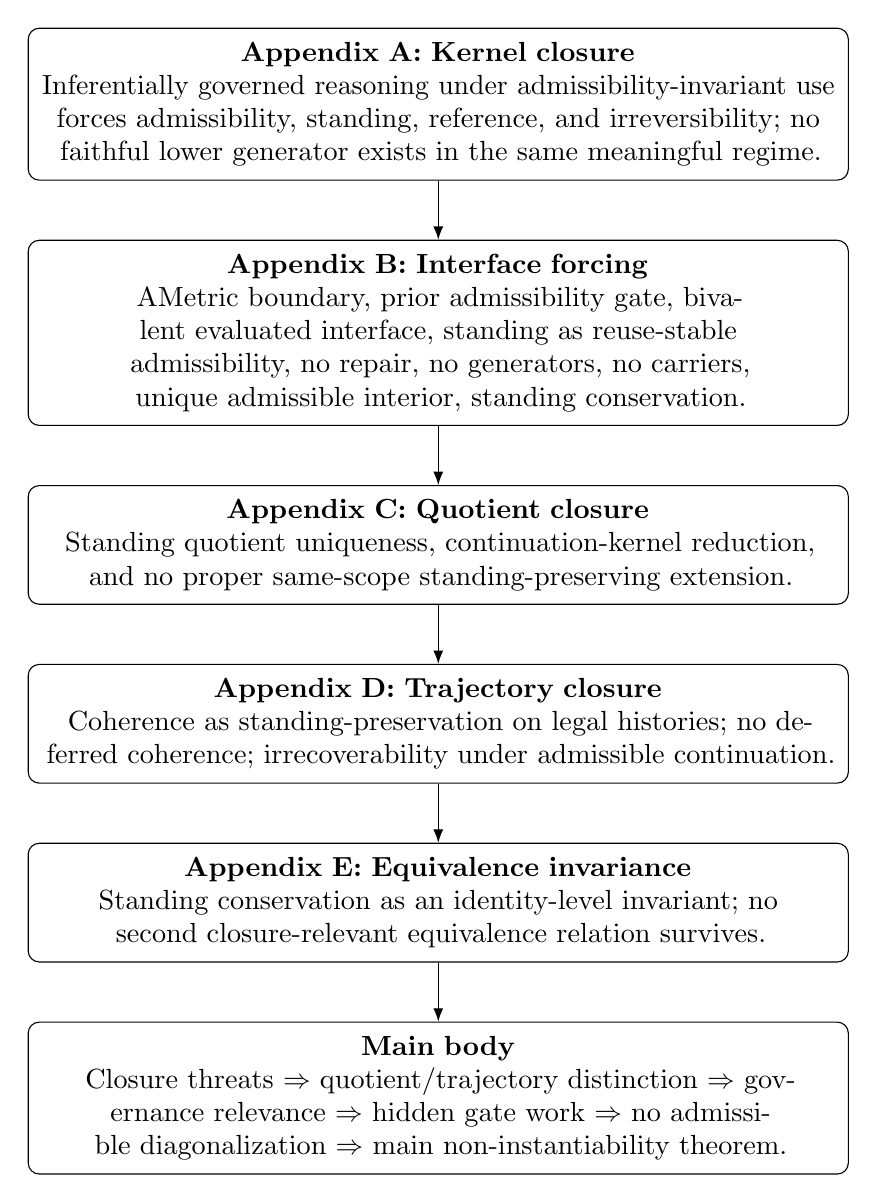
\begin{tikzpicture}[node distance=0.75cm, every node/.style={draw, rounded corners, align=center, inner sep=5pt, text width=0.83\linewidth}, >=Latex]
\node (k) {\textbf{Appendix A: Kernel closure}\\Inferentially governed reasoning under admissibility-invariant use forces admissibility, standing, reference, and irreversibility; no faithful lower generator exists in the same meaningful regime.};
\node (i) [below=of k] {\textbf{Appendix B: Interface forcing}\\AMetric boundary, prior admissibility gate, bivalent evaluated interface, standing as reuse-stable admissibility, no repair, no generators, no carriers, unique admissible interior, standing conservation.};
\node (q) [below=of i] {\textbf{Appendix C: Quotient closure}\\Standing quotient uniqueness, continuation-kernel reduction, and no proper same-scope standing-preserving extension.};
\node (t) [below=of q] {\textbf{Appendix D: Trajectory closure}\\Coherence as standing-preservation on legal histories; no deferred coherence; irrecoverability under admissible continuation.};
\node (e) [below=of t] {\textbf{Appendix E: Equivalence invariance}\\Standing conservation as an identity-level invariant; no second closure-relevant equivalence relation survives.};
\node (g) [below=of e] {\textbf{Main body}\\Closure threats $\Rightarrow$ quotient/trajectory distinction $\Rightarrow$ governance relevance $\Rightarrow$ hidden gate work $\Rightarrow$ no admissible diagonalization $\Rightarrow$ main non-instantiability theorem.};
\draw[->] (k) -- (i);
\draw[->] (i) -- (q);
\draw[->] (q) -- (t);
\draw[->] (t) -- (e);
\draw[->] (e) -- (g);
\end{tikzpicture}
\caption{Dependency map for the self-contained audit edition. Every theorem family used by the main G\"odel result is reproved in the appendices.}
\label{fig:dependency-map}
\end{figure}

The paper is intentionally conservative in what it claims. It does \emph{not} assert global completeness, refute classical incompleteness, or prohibit all external metamathematical coding. It proves a structural exclusion result: within the unique admissible interior of the fixed regime defined in the appendices, a G\"odel architecture relevant to same-domain governance-level closure is not instantiable.

\section{Roadmap and in-paper package}
\label{sec:roadmap}

We work throughout over a fixed meaningful regime and a fixed domain $\domain$ with evaluated fragment $\Eval$. Lawful redescription is written $\Law$. The appendices establish the following in-paper package; these are the only upstream facts used in the main theorem chain.

\begin{enumerate}[label=\textbf{(P\arabic*)}, leftmargin=3.1em]
    \item \textbf{Kernel closure.} Inferentially governed proposition-bearing reasoning under admissibility-invariant use has a minimal assessability boundary; non-degenerate reasoning forces admissibility, standing, reference, and irreversibility; and no faithful lower generator of these governance conditions exists either inside the same meaningful regime or in any faithful same-domain extension (\cref{thm:A-assessability,thm:A-kernel,thm:A-regime-invariant,cor:A-no-lower-generator}).

    \item \textbf{AMetric boundary, no deeper invariant, and prior gate.} On the pre-admissible side there is no admissibility-relevant grading, selector, ranking, or nontrivial metric; no deeper pre-boundary invariant survives with independent constraining force; and a prior admissibility gate is forced only after failure-class exhaustion closes every evasion route (\cref{thm:B-ametric,thm:B-no-deeper-invariant,thm:B-failure-exhaustion,thm:B-failure-collapse,thm:B-gate-necessity}).

    \item \textbf{Bivalence and unique gate classification.} Every admissibility-relevant status interface on $\domain$ collapses extensionally to admitted/not-admitted via an exhaustive same-side split trichotomy, and two lawful-redescription-invariant same-domain gates cannot disagree extensionally (\cref{lem:B-trichotomy,prop:B-no-redescription-split,prop:B-no-effective-split,prop:B-inert-collapse,thm:B-bivalence,cor:B-unique-gate}).

    \item \textbf{Standing emergence and conservation.} Standing is exactly reuse-stable admissibility on the fixed domain; admitted same-scope continuation preserves the standing-relevant invariant bundle; there is no same-act repair, no generator, no independent carrier, no plurality of same-scope interiors, and no same-domain creation, amplification, transfer, or recovery of standing without fresh gating (\cref{prop:B-preserve-invariants,thm:B-standing,thm:B-no-repair,thm:B-no-generators,thm:B-no-carriers,thm:B-interior-unique,thm:B-conservation}).

    \item \textbf{No semantic or infinitary standing import.} Truth, satisfaction, ``all models,'' reflection, and infinitary rule-power cannot serve as independent same-domain standing-bearing authorizers (\cref{prop:B-no-semantic-import}).

    \item \textbf{Standing quotient uniqueness.} Any same-domain standing presentation is sound and complete exactly when it factors through the standing quotient; that quotient is unique up to unique isomorphism (\cref{thm:C-quotient-unique}).

    \item \textbf{Continuation-kernel maximality.} Every same-domain standing-preserving map factors uniquely through the standing quotient, and there is no proper same-domain standing-preserving extension beyond the quotient (\cref{thm:C-factor,thm:C-no-proper-extension}).

    \item \textbf{Trajectory closure.} Coherence of a legal same-domain trajectory is pointwise standing-preservation; incoherent prefixes remain incoherent under extension; standing failure is irrecoverable downstream (\cref{thm:D-prefix,thm:D-no-deferred,thm:D-irrecoverable,thm:D-terminal}).

    \item \textbf{Equivalence invariance.} Standing conservation is an identity-level invariant of admissible classification; no second closure-relevant equivalence relation survives alongside admissible standing classification (\cref{thm:E-conservation,thm:E-no-second-equivalence}).
\end{enumerate}

The main theorem chain will cite only these in-paper labels. In particular, the main body now uses this package to derive an explicit prerequisite-exhaustion theorem for any same-domain G\"odel threat before diagonalization is attempted.

\subsection{Formalization status for the present manuscript}
\label{sec:formalization-status-main}

The present manuscript is auditable in two exact forms. First, it is an in-paper theorem package whose proof force is carried entirely by the labeled results reproduced here. Second, the theorem chain of this manuscript has been encoded in Lean4 with the same proof order: from the imported primitive appendix package through inferential-exhaustion, code-role exhaustion, G\"odel-prerequisite exhaustion, rescue-route exhaustion, and the terminal non-instantiability theorem. The formalization is explicitly scoped to this paper. It does not here serve as a claim about other downstream manuscripts.

Just as the paper does not attempt to derive its primitive floor from below, the Lean development does not treat that floor as a theorem to be generated internally. Instead it assumes the same primitive appendix package used by the manuscript and formally derives the main-body theorem chain built on that floor. Appendix~\ref{app:formalization-status} records the paper-to-Lean correspondence for the present manuscript, including the exported paper-facing theorem names whose axiom audits return no axioms and the certified ledger statement aligning the imported appendix labels used by this paper with the primitive package used by the formal development.

\section{Fixed-domain closure threats and G\"odel architectures}
\label{sec:threats}

We now define precisely what kind of G\"odel-style construction could even count as a threat to governance-level closure.

\begin{definition}[Instantiability on a fixed domain]
A structure $\mathcal{S}$ is \emph{instantiable on $\domain$} if all objects, maps, predicates, equivalences, and readback operations required by $\mathcal{S}$ exist within the same meaningful regime on $\domain$ and perform the roles assigned to them without explicit scope reset or domain change.
\end{definition}

\begin{definition}[Same-domain faithful coding layer]
Fix a class $A \subseteq \Eval$ of syntax-bearing acts. A coding layer for $A$ on $\domain$ consists of a class $C$ of code-objects together with a coding map
\[
\code{\cdot}:A\to C.
\]
The coding layer is \emph{same-domain faithful} if predicates on $C$ may be used, without explicit scope reset or domain change, to formulate standing-bearing claims about the original acts in $A$ and to constrain their admissible reuse or continuation on $\domain$.
\end{definition}

\begin{definition}[Readback of a code-predicate]
Let $P\subseteq C$ be a predicate on code-objects. Its \emph{same-domain readback} is the induced predicate
\[
\widehat P(a):\Longleftrightarrow P(\code{a})
\qquad (a\in A),
\]
whenever this induced predicate is claimed to govern admissibility, standing, or standing-bearing continuation of the original acts on $\domain$.
\end{definition}

\begin{definition}[Content carrier and lawful content equivalence]
Fix a content carrier $\mathcal{L}_{\domain}$ for the fixed domain together with a content assignment
\[
\kappa:A\to \mathcal{L}_{\domain}.
\]
A binary relation $\equiv_{\domain}$ on $\mathcal{L}_{\domain}$ is a \emph{lawful content equivalence} if whenever $\kappa(a)\equiv_{\domain}\kappa(b)$, replacing $a$ by $b$ changes neither standing classification nor any legal same-domain trajectory status. We say that two acts have the same \emph{standing-bearing content up to lawful equivalence} when their contents are equivalent under $\equiv_{\domain}$.
\end{definition}

\begin{remark}[Typing convention for content claims]
When the paper says that an act $g$ has standing-bearing content lawfully equivalent to a formula such as $\neg P(\code{g})$, the precise claim is that there exists an element $\varphi_g\in \mathcal{L}_{\domain}$ with $\kappa(g)\equiv_{\domain}\varphi_g$, and $\varphi_g$ is the internal content-token corresponding to the indicated formula. All appeals to ``lawful equivalence of content'' are to this typed relation.
\end{remark}

\begin{definition}[Inferential life of the fixed domain]
The \emph{inferential life} of the fixed domain $\domain$ is the totality of what may be admitted, rejected, committed, reused, or licensed as same-domain continuation on $\domain$.
\end{definition}

\begin{definition}[Closure threat on a fixed domain]
A distinction, sentence, or construction $\Theta$ is a \emph{closure threat on $\domain$} if, without explicit scope change, its presence or absence changes the inferential life of the fixed domain. A distinction that changes no such inferential fact is \emph{closure-inert} on $\domain$.
\end{definition}

\begin{definition}[Governance-relevant code-predicate]
A code-predicate $P\subseteq C$ is \emph{governance-relevant on $\domain$} if its same-domain readback $\widehat P$ is not closure-inert, i.e. if $\widehat P$ changes the inferential life of the fixed domain.
\end{definition}

\begin{definition}[G\"odel apparatus on the fixed domain]
A \emph{G\"odel apparatus on $\domain$} consists of:
\begin{enumerate}[label=(\alph*), leftmargin=2.5em]
    \item a same-domain faithful coding layer $\code{\cdot}:A\to C$;
    \item a governance-relevant code-predicate $\Prov\subseteq C$ intended to play the role of internal provability or code-level authorization;
    \item a substitution/diagonal mechanism that can produce an act $g\in A$ together with a content-token $\varphi_g\in \mathcal{L}_{\domain}$ such that $\kappa(g)\equiv_{\domain}\varphi_g$ and $\varphi_g$ is a negative fixed-point formula of the form $\neg \Prov(\code{g})$.
\end{enumerate}
Such an apparatus is a \emph{G\"odel threat} if it is claimed to be a closure threat on $\domain$.
\end{definition}

The first load-bearing question is: when does an undecidability phenomenon matter to closure at all?

\begin{lemma}[Fixed-domain inferential-life exhaustion]
\label{lem:inferential-life-exhaustion}
On the fixed domain $\domain$, inferential life is exhausted by two structures:
\begin{enumerate}[label=(\roman*), leftmargin=2.5em]
    \item the standing classification of evaluated acts in $\Eval$; and
    \item the terminal standing behavior of legal same-domain trajectories in $\Traj$.
\end{enumerate}
More precisely: if two same-domain governance descriptions agree on the standing classification of every evaluated act and on the terminal standing behavior of every legal same-domain trajectory, then they agree on what may be admitted, rejected, reused, committed, or licensed as same-domain continuation on $\domain$.
\end{lemma}

\begin{proof}
At the act level, \cref{thm:B-standing,cor:B-unique-gate} identify standing with reuse-stable admissibility and rule out any second same-domain gate with different extension. Moreover, \cref{thm:C-quotient-unique,thm:C-no-proper-extension} show that every same-domain standing-preserving presentation factors uniquely through the standing quotient and adds no further standing-bearing content beyond admissible standing classes, while \cref{thm:E-no-second-equivalence} rules out any second closure-relevant equivalence relation alongside admissible standing classification. So once standing classification of evaluated acts is fixed, no additional act-level same-domain inferential distinction remains.

At the trajectory level, \cref{lem:D-failure,thm:D-no-deferred,thm:D-irrecoverable,thm:D-terminal} show that coherence of a legal same-domain trajectory is fixed by failure-witness structure and terminal standing, and that same-domain continuation cannot retrospectively repair a failure inside the retained lineage. Therefore once terminal standing behavior of legal same-domain trajectories is fixed, what may be licensed as same-domain continuation or commitment is fixed as well.

Since the inferential life of $\domain$ consists exactly of what may be admitted, rejected, reused, committed, or licensed as same-domain continuation, agreement on (i) and (ii) exhausts it.
\end{proof}

\begin{lemma}[Closure-relevance transmission]
\label{lem:closure-transmission}
Let $\Theta$ be any same-domain distinction on the fixed domain $\domain$. If $\Theta$ changes the inferential life of $\domain$, then $\Theta$ changes at least one of the following:
\begin{enumerate}[label=(\roman*), leftmargin=2.5em]
    \item the standing classification of some evaluated act in $\Eval$; or
    \item the terminal standing behavior, and hence the licensed continuation structure, of some legal same-domain trajectory in $\Traj$.
\end{enumerate}
\end{lemma}

\begin{proof}
Assume that $\Theta$ changes neither the standing classification of any evaluated act nor the terminal standing behavior of any legal same-domain trajectory. Then any same-domain governance description with $\Theta$ and without $\Theta$ agrees on exactly the two structures isolated in \cref{lem:inferential-life-exhaustion}. By that lemma, the two descriptions therefore agree on the inferential life of the fixed domain. This contradicts the hypothesis that $\Theta$ changes inferential life. Hence at least one of (i) or (ii) must occur.
\end{proof}

\begin{theorem}[Inferential Necessity of Closure Distinctions]
\label{thm:inferential-necessity}
Let $F$ be a formal system associated with the fixed domain $\domain$, and let $\Theta$ be a sentence, code-construction, or metamathematical distinction formulated in $F$. Suppose the claim is that the undecidability, unprovability, or fixed-point behavior of $\Theta$ undercuts closure of reasoning on $\domain$ in the ordinary inferential sense: namely, it changes what may be consistently admitted, rejected, committed, or licensed as same-domain continuation when $\Theta$ is used in reasoning on $\domain$. Then $\Theta$ must induce at least one of the following:
\begin{enumerate}[label=(\roman*), leftmargin=2.5em]
    \item a difference in the standing classification of some evaluated act in $\Eval$; or
    \item a difference in the terminal standing of at least one legal same-domain trajectory in $\Traj$, equivalently a divergence in what may be licensed as standing-bearing continuation or commitment on $\domain$.
\end{enumerate}
Consequently, every standard G\"odel-style phenomenon can threaten closure on $\domain$ only if it survives into the standing quotient or coherent trajectory structure of the fixed domain.
\end{theorem}

\begin{proof}
By hypothesis, the presence or absence of $\Theta$ changes the inferential life of the fixed domain. Therefore \cref{lem:closure-transmission} yields either a standing-classification difference or a trajectory-level terminal-standing difference.

If the difference is of type (i), then by \cref{thm:C-quotient-unique,thm:E-no-second-equivalence} it survives into the standing quotient: there is no second closure-relevant equivalence relation on the fixed domain that could absorb the distinction while leaving admissible standing classification unchanged.

If the difference is of type (ii), then by \cref{thm:D-terminal,thm:D-no-deferred,thm:D-irrecoverable} it survives into coherent trajectory structure itself: terminal standing certifies coherence, incoherent prefixes remain incoherent under extension, and standing failure cannot be repaired downstream within the same lineage.

Therefore every standard G\"odel-style phenomenon that genuinely threatens closure on $\domain$ must survive into the standing quotient or coherent trajectory structure of the fixed domain.
\end{proof}

\begin{corollary}[External undecidability inertness]
\label{cor:external-inert}
An undecidable or unprovable sentence that never re-enters the fixed domain so as to change the standing classification of an evaluated act or the terminal standing behavior of a legal same-domain trajectory is closure-inert on $\domain$.
\end{corollary}

\begin{proof}
If neither kind of change occurs, then \cref{lem:closure-transmission} shows that the distinction does not change the inferential life of the fixed domain. Hence it is not a closure threat.
\end{proof}

\begin{corollary}[Trajectory-neutral closure relevance is act-level]
\label{cor:trajectory-neutral}
If an alleged distinction on $\domain$ alters no legal same-domain trajectory---equivalently, changes neither any terminal standing outcome nor any licensed same-domain continuation---then any closure relevance it has must appear as a difference in standing classification of some evaluated act.
\end{corollary}

\begin{proof}
Apply \cref{lem:closure-transmission}. If clause (ii) is absent by hypothesis, only clause (i) remains.
\end{proof}

\begin{remark}[Why G\"odel must become governance-relevant to matter]
Classical incompleteness by itself is not enough to threaten closure in the present sense. To matter here, the undecidable or unprovable sentence must change the inferential life of the fixed domain; and by \cref{lem:closure-transmission,thm:inferential-necessity}, any such change must survive into standing classification or coherent trajectory structure. The bridge from standard metamathematical talk to governance-level closure is therefore theorematic rather than interpretive.
\end{remark}

\section{Governance-relevant code-predicates are hidden gate work}
\label{sec:predicates}

Once a code-predicate is asked to matter to closure on the same fixed domain, it is no longer innocent bookkeeping. The next theorem formalizes that point.

\begin{lemma}[Hidden gate-work lemma]
\label{lem:hidden-gate}
Let $P\subseteq C$ be a code-predicate in a same-domain faithful coding layer with readback $\widehat P$ on $A\subseteq \Eval$. If $\widehat P$ is governance-relevant on $\domain$, then $\widehat P$ performs hidden gate work on the original fixed domain: it either
\begin{enumerate}[label=(\roman*), leftmargin=2.5em]
    \item changes which acts are admitted or standing-positive on $\domain$; or
    \item refines the positive side or negative side of the gate into a further substantive same-domain classification affecting licensed continuation.
\end{enumerate}
\end{lemma}

\begin{proof}
If $\widehat P$ is governance-relevant, then by definition it changes the inferential life of the fixed domain. By \cref{thm:inferential-necessity}, that inferential difference must appear either as a standing-classification difference for some evaluated act or as a trajectory-level difference in licensed same-domain continuation. If it changes whether an act is admitted or standing-positive, then it directly changes the gate on the original fixed domain, giving (i). If it leaves admission unchanged but changes what later same-domain continuation or commitment is licensed, then it creates a substantive same-side refinement inside the positive or negative side of the gate, giving (ii). There is no third possibility, because \cref{thm:inferential-necessity} has already exhausted the closure-relevant loci.
\end{proof}

\begin{theorem}[Exhaustion of same-domain code-predicate roles]
\label{thm:code-role-exhaustion}
Let $P\subseteq C$ be a code-predicate in a same-domain faithful coding layer with readback $\widehat P$ on $A\subseteq \Eval$. Then exactly one of the following roles is instantiated on the fixed domain $\domain$:
\begin{enumerate}[label=(\roman*), leftmargin=2.5em]
    \item \textbf{Inert bookkeeping:} $\widehat P$ is closure-inert and changes neither standing classification nor licensed same-domain continuation.
    \item \textbf{Extensional gate renaming:} $\widehat P$ coincides extensionally with the unique admissibility gate (equivalently, with standing on the evaluated fragment) and therefore contributes no independent governance work.
    \item \textbf{Same-side refinement:} $\widehat P$ leaves gate verdicts unchanged but purports to refine the admitted side or rejected side into a further substantive same-domain classification affecting licensed continuation.
    \item \textbf{Independent standing-bearing authorizer:} $\widehat P$ purports to authorize admissibility or standing-bearing continuation independently of the unique gate and is not extensionally identical with it.
\end{enumerate}
No fifth same-domain governance role exists.
\end{theorem}

\begin{proof}
Fix $P\subseteq C$ with readback $\widehat P$.

If $\widehat P$ is closure-inert, then role~(i) holds by definition.

Assume instead that $\widehat P$ is governance-relevant. By \cref{lem:hidden-gate}, $\widehat P$ performs hidden gate work on the original fixed domain. There are then only two possibilities.

First, $\widehat P$ changes which acts are admitted or standing-positive on $\domain$. In that case either the induced classification agrees extensionally with the unique gate, yielding role~(ii), or it does not agree extensionally, yielding role~(iv).

Second, $\widehat P$ leaves admission unchanged but changes what later same-domain continuation or commitment is licensed. Then it refines the positive or negative side of the gate into a further substantive same-domain classification, which is exactly role~(iii).

These cases are mutually exclusive. Role~(i) excludes governance relevance altogether. Role~(ii) requires extensional coincidence with the unique gate, whereas role~(iv) requires non-coincidence. Role~(iii) leaves admission fixed while roles~(ii) and~(iv) are gate-level cases. Thus no fifth role remains.
\end{proof}

\begin{proposition}[Gate-renaming collapse]
\label{prop:gate-renaming-collapse}
If a same-domain code-predicate instantiates role~\textup{(ii)} of \cref{thm:code-role-exhaustion}, then its readback is extensional renaming only: it adds no independent governance content beyond the unique gate.
\end{proposition}

\begin{proof}
Role~(ii) states that $\widehat P$ coincides extensionally with the unique admissibility gate on the evaluated fragment. Since \cref{cor:B-unique-gate} rules out any second same-domain gate classification on the same fixed scope, extensional coincidence exhausts the standing-bearing content of $\widehat P$. Any residual distinction is therefore bookkeeping only.
\end{proof}

\begin{proposition}[Same-side refinement is impossible]
\label{prop:same-side-refinement-impossible}
No same-domain code-predicate can instantiate role~\textup{(iii)} of \cref{thm:code-role-exhaustion}.
\end{proposition}

\begin{proof}
Role~(iii) says that admission is unchanged but that some further substantive same-domain classification on the positive side or negative side changes licensed continuation. By \cref{lem:hidden-gate}, that is hidden gate work. In Appendix~B, effective same-side splits are eliminated: a substantive refinement on the admitted side or rejected side is impossible by \cref{prop:B-no-effective-split}. Equivalently, such a refinement would either introduce deferred gate work inside the positive side or open a same-scope promotion channel inside the negative side, both of which are barred on the fixed domain. Hence role~(iii) cannot be instantiated.
\end{proof}

\begin{proposition}[Independent same-domain authorizers are impossible]
\label{prop:independent-authorizer-impossible}
No same-domain code-predicate can instantiate role~\textup{(iv)} of \cref{thm:code-role-exhaustion}.
\end{proposition}

\begin{proof}
Role~(iv) says that the readback of the code-predicate functions as a standing-bearing authorizer that is not extensionally identical with the unique gate. If it changes which acts are admitted or standing-positive, then it contradicts the uniqueness of gate classification on the fixed domain given by \cref{cor:B-unique-gate}. If it purports to remain standing-bearing without directly changing admission, then it is an independent carrier beneath standing, contradicting \cref{thm:B-no-carriers}. Thus role~(iv) is impossible.
\end{proof}

\begin{theorem}[No independent governance-relevant code-predicate]
\label{thm:no-code-predicate}
No code-predicate $P\subseteq C$ can serve as an independent governance-relevant authorizer on the original fixed domain $\domain$. Every same-domain code-predicate is therefore either inert bookkeeping or extensional renaming of the unique admissibility gate.
\end{theorem}

\begin{proof}
By \cref{thm:code-role-exhaustion}, every same-domain code-predicate must instantiate exactly one of the four roles listed there. \Cref{prop:gate-renaming-collapse,prop:same-side-refinement-impossible,prop:independent-authorizer-impossible} eliminate roles~(ii)--(iv) as sources of independent governance force. Thus the only surviving possibilities are inert bookkeeping or extensional gate renaming. In particular, no independent governance-relevant code-predicate exists.
\end{proof}

\begin{corollary}[One numbering is not enough]
\label{cor:one-numbering}
A single fixed coding map does not by itself evade \cref{thm:no-code-predicate}. Even one numbering is harmless unless predicates on its codes re-enter the original fixed domain as governance-relevant constraints; and once they do, \cref{thm:code-role-exhaustion,thm:no-code-predicate} apply.
\end{corollary}

\begin{proof}
The danger is not multiplicity of numbering as such, but governance-relevant readback. A single numbering that never changes standing or trajectories is closure-inert by \cref{cor:external-inert}. A single numbering that does change them yields a governance-relevant code-predicate, whose only same-domain roles are exhausted by \cref{thm:code-role-exhaustion}; the only surviving roles are bookkeeping or extensional gate renaming by \cref{thm:no-code-predicate}.
\end{proof}

\begin{lemma}[Representational differences are either inert or inferential]
\label{lem:representation-difference}
Let $r_1$ and $r_2$ be same-domain presentations of the same evaluated act $a\in\Eval$. Then exactly one of the following holds:
\begin{enumerate}[label=(\roman*), leftmargin=2.5em]
    \item the difference between $r_1$ and $r_2$ is lawfully equivalent or closure-inert and therefore collapses as bookkeeping; or
    \item the difference changes standing classification of some evaluated act or alters legal same-domain trajectory structure, and so is inferential rather than merely representational.
\end{enumerate}
\end{lemma}

\begin{proof}
If the representational difference is closure-inert, then by \cref{cor:external-inert} it changes no standing fact and no legal same-domain continuation fact, so it is bookkeeping only. If it is not closure-inert, then by \cref{thm:inferential-necessity} it must survive into standing classification or coherent trajectory structure. Those are exactly the inferentially relevant cases.
\end{proof}

\begin{theorem}[No non-trivial admissible encoding multiplicity]
\label{thm:no-encoding-multiplicity}
Fix an evaluated act $a\in\Eval$. There is no non-trivial same-domain admissible multiplicity of governance-relevant representations of $a$. More precisely: if two representations $r_1,r_2$ of $a$ are both admitted as same-domain governance-relevant presentations, then either
\begin{enumerate}[label=(\roman*), leftmargin=2.5em]
    \item $r_1$ and $r_2$ are lawfully equivalent presentations and hence induce no distinct admissibility-relevant content; or
    \item at least one of $r_1,r_2$ is not admissible as a same-domain governance-relevant representation of $a$.
\end{enumerate}
\end{theorem}

\begin{proof}
Assume that $r_1$ and $r_2$ are two admitted same-domain governance-relevant representations of the same evaluated act $a$ and are not lawfully equivalent. By \cref{lem:representation-difference}, either their difference is closure-inert, in which case we are in case~(i) after quotienting away inert presentation difference, or their difference alters standing classification or legal same-domain trajectory structure.

Suppose the latter. Because the represented act is still the same evaluated act $a$, any such standing- or trajectory-level difference is a same-domain representational refinement only. But \cref{thm:E-no-second-equivalence} forbids any second closure-relevant equivalence relation beside standing-equivalence, and \cref{thm:C-no-proper-extension} forbids any proper same-domain standing-preserving extension beyond the standing quotient. Therefore the representational difference cannot carry independent same-domain standing content. So at least one of $r_1,r_2$ is inadmissible as a governance-relevant representation of $a$, yielding case~(ii).
\end{proof}


\section{Diagonalization and rescue-route exhaustion}
\label{sec:diagonal}

A G\"odel architecture needs more than codes. It needs a finite same-domain prerequisite package: code-level distinctions must come back to govern the original domain, those code-level distinctions must survive the role-exhaustion theorems of Section~\ref{sec:predicates}, and a negative fixed-point construction must then produce an act whose standing-bearing content denies its own admissibility through its code. The following definitions and theorems make that prerequisite package explicit and then show that every same-domain realization of it collapses.

\begin{definition}[Same-domain negative fixed-point construction]
A same-domain diagonal apparatus on $\domain$ consists of:
\begin{enumerate}[label=(\alph*), leftmargin=2.5em]
    \item a same-domain faithful coding map $\code{\cdot}:A\to C$;
    \item a governance-relevant code-predicate $P\subseteq C$ with readback $\widehat P$;
    \item an admissible substitution/readback operation $\Delta$ such that for some $g\in A$, the standing-bearing content of $g$ is lawfully equivalent to a formula of the form $\neg P(\code{g})$, or more generally to a fixed-point statement about its own code.
\end{enumerate}
\end{definition}

\begin{theorem}[Necessary package for a same-domain G\"odel threat]
\label{thm:godel-prerequisites}
Let $F$ be any formal system or coding architecture associated with the fixed domain $\domain$. If a G\"odel-style undecidability, unprovability, or fixed-point phenomenon in $F$ is claimed to threaten governance-level closure on $\domain$ from within the same domain, then any such same-domain realization requires all of the following simultaneously:
\begin{enumerate}[label=(\roman*), leftmargin=2.5em]
    \item a same-domain faithful coding layer on some class $A\subseteq \Eval$;
    \item governance-relevant readback of at least one code-predicate, code-construction, or equivalent code-based distinction to the original fixed domain;
    \item a standing-bearing code-predicate role that is not closure-inert and so must survive the code-role exhaustion package of Section~\ref{sec:predicates};
    \item an admissible same-domain fixed-point production yielding an act $g\in A$ whose standing-bearing content is lawfully equivalent to a negative fixed-point formula over its own code; and
    \item survival of the resulting distinction into the standing quotient or coherent trajectory structure of $\domain$.
\end{enumerate}
\end{theorem}

\begin{proof}
If there is no same-domain faithful coding layer, then there is no same-domain coding architecture through which code-judgments can re-enter the original fixed domain at all, so the alleged G\"odel phenomenon remains external bookkeeping.

If there is no governance-relevant readback, then whatever code-level distinction is being studied changes no standing fact and no licensed same-domain continuation fact on $\domain$; by \cref{cor:external-inert} it is closure-inert.

If the readback is governance-relevant but does not present itself as a standing-bearing code-predicate role, then there is no same-domain standing-bearing authorizer or gate-relevant constraint for the code level to contribute on the original domain. Section~\ref{sec:predicates} makes this precise by exhausting the possible same-domain roles of code-predicates.

If there is no admissible same-domain fixed-point production, then there is no G\"odel-style negative self-reference on the original fixed domain, but only external coding without internal diagonal re-entry.

Finally, if the resulting distinction does not survive into the standing quotient or coherent trajectory structure, then by \cref{thm:inferential-necessity} it does not threaten governance-level closure on $\domain$.

Thus every same-domain G\"odel threat must realize all five items simultaneously.
\end{proof}

\begin{theorem}[Exhaustion of same-domain self-reference prerequisites]
\label{thm:self-reference-prereqs}
Assume the prerequisite package of \cref{thm:godel-prerequisites}. Then exactly one of the following holds for the governing code-predicate role on the fixed domain $\domain$:
\begin{enumerate}[label=(\roman*), leftmargin=2.5em]
    \item the readback is closure-inert, so the putative self-reference is closure-inert and not a same-domain G\"odel threat;
    \item the readback is extensional gate renaming, so any remaining same-domain self-reference candidate collapses to a gate-collapsed negative fixed point of the form ``not admitted'' or ``not standing-positive'';
    \item the readback is same-side refinement or independent authorizer, both of which are impossible on the fixed domain.
\end{enumerate}
Consequently, after code-role exhaustion the only remaining governance-relevant same-domain self-reference candidate is the gate-collapsed negative fixed point.
\end{theorem}

\begin{proof}
By \cref{thm:code-role-exhaustion}, every same-domain code-predicate role is exactly one of inert bookkeeping, extensional gate renaming, same-side refinement, or independent standing-bearing authorizer.

If the role is inert bookkeeping, then the readback is closure-inert by definition, yielding case~(i).

If the role is extensional gate renaming, then the code-predicate contributes no governance content beyond the unique gate by \cref{prop:gate-renaming-collapse}. In that case any negative fixed point over the code-predicate is, extensionally, a negative fixed point over the gate itself, yielding case~(ii).

If the role is same-side refinement, then \cref{prop:same-side-refinement-impossible} rules it out. If the role is independent authorizer, then \cref{prop:independent-authorizer-impossible} rules it out. These are exactly the impossible branches in case~(iii).

No fifth self-referential prerequisite remains because no fifth same-domain code-predicate role exists.
\end{proof}

\begin{theorem}[Non-existence of admissible same-domain diagonalization]
\label{thm:no-diagonalization}
No same-domain diagonal apparatus producing a governance-relevant negative fixed point is instantiable on the fixed domain $\domain$.
\end{theorem}

\begin{proof}
Assume, for contradiction, that a same-domain diagonal apparatus exists. By \cref{thm:godel-prerequisites}, it must realize a same-domain faithful coding layer, governance-relevant readback, a standing-bearing code-predicate role, an admissible negative fixed-point production, and survival of the resulting distinction into the standing quotient or coherent trajectory structure. By \cref{thm:self-reference-prereqs}, the only remaining governance-relevant self-reference candidate after code-role exhaustion is the gate-collapsed case.

So there exists an act $g\in A$ whose standing-bearing content is lawfully equivalent to $\neg P(\code{g})$, where the readback of $P$ coincides extensionally with the unique admissibility gate on the fixed domain. Equivalently, the standing-bearing content of $g$ is lawfully equivalent to ``$g$ is not admitted'' or ``$g$ is not standing-positive.'' We now derive an exhaustive contradiction.

\emph{Case 1: $g$ is admitted / standing-positive.} Then by standing emergence, $g$ is reuse-stably admissible by \cref{thm:B-standing}. But the content tracked by $g$ says that $g$ is not admitted. Lawful redescription invariance forces the same fixed-domain classification on lawfully equivalent presentations; so admission of $g$ implies non-admission of $g$. This contradicts bivalence and unique gate classification from \cref{thm:B-bivalence,cor:B-unique-gate}. More explicitly, the same evaluated act would be both admitted and not admitted on the same fixed scope.

\emph{Case 2: $g$ is not admitted / not standing-positive.} Then $g$ carries no standing-bearing force on the fixed domain. For the fixed point nevertheless to threaten closure, its negative status would have to be reversed or made governance-relevant again by one of two routes.

\emph{Case 2a: same-act repair or generation.} Any same-scope attempt to restore force to $g$ as the same evaluated act is barred by \cref{thm:B-no-repair}. Any attempt to produce standing-positive force from the failed act alone without fresh gating is barred by \cref{thm:B-no-generators}. Any attempt to authorize such restoration by a derived predicate is barred by \cref{thm:B-no-carriers}.

\emph{Case 2b: downstream restoration within the same lineage.} If one tries to make the failed fixed point matter by later same-domain continuation while retaining that lineage, then the lineage already contains a standing failure. By \cref{thm:D-no-deferred,thm:D-irrecoverable}, once an incoherent prefix appears, no admissible continuation restores coherence, and standing failure propagates irrecoverably downstream within the same lineage.

These cases exhaust the ways a non-standing negative fixed point could regain same-domain governance force. Since every such route is blocked, the fixed point in Case~2 is closure-inert, contradicting item~(v) of \cref{thm:godel-prerequisites}.

In either case the supposed same-domain diagonal apparatus fails to instantiate a governance-relevant threat. Therefore no admissible same-domain diagonalization exists.
\end{proof}
\begin{corollary}[No governance-relevant negative fixed point]
\label{cor:no-negative-fixedpoint}
There is no governance-relevant fixed-domain act $g$ whose standing-bearing content is lawfully equivalent to $\neg \Prov(\code{g})$ for any same-domain provability predicate $\Prov$.
\end{corollary}

\begin{proof}
Such an act is exactly a governance-relevant negative fixed point and therefore part of a same-domain negative fixed-point construction. \Cref{thm:no-diagonalization} eliminates that possibility.
\end{proof}

\paragraph{Semantic, infinitary, and extension rescue-route exhaustion.}
The diagonal no-go closes the same-domain coding and self-reference package. A hostile reader may still try to reopen the threat by semantic truth, intended-model talk, infinitary rule-power, or richer same-domain extension. We therefore classify those rescue routes explicitly before turning to the main theorem.

\begin{theorem}[No semantic standing import on the fixed domain]
\label{thm:no-semantic-import}
Truth, satisfaction, ``all models,'', intended-model semantics, and semantic consequence cannot function as independent same-domain standing-bearing authorizers on the fixed domain $\domain$. Any same-domain appeal to such resources is therefore either closure-inert bookkeeping, extensional gate renaming, or explicit scope change.
\end{theorem}

\begin{proof}
By \cref{prop:B-no-semantic-import}, truth, satisfaction, ``all models,'' reflection, and analogous semantic resources cannot serve as independent same-domain standing-bearing authorizers on the fixed domain. If a semantic appeal changes no standing classification and no coherent trajectory fact, then by \cref{cor:external-inert} it is closure-inert bookkeeping.

Assume instead that a semantic appeal is claimed to matter to governance-level closure on the same fixed domain. Then by \cref{thm:inferential-necessity} it must survive into standing classification or coherent trajectory structure. If it agrees extensionally with the unique gate on the evaluated fragment, then by \cref{cor:B-unique-gate} it contributes no new same-domain authority and is only extensional gate renaming. If it does not agree extensionally with that gate, then it functions as an independent same-domain authorizer, which \cref{prop:B-no-semantic-import} forbids. The only remaining way to make semantic resources matter is to move to a new scope, a new domain, or fresh gating, which is outside the present same-domain claim.
\end{proof}

\begin{definition}[Meta-foundational re-anchoring on the old scope]
A \emph{same-domain meta-foundational re-anchoring} is any attempt to authorize admissibility, standing, or standing-bearing continuation on the original fixed domain by appeal to a truth predicate, satisfaction predicate, global closure predicate, foundation swap, intended semantics, or comparable meta-level resource that is not already extensionally identical with the unique same-domain gate.
\end{definition}

\begin{theorem}[No meta-foundational re-anchoring on the old scope]
\label{thm:no-meta-reanchoring}
No same-domain meta-foundational re-anchoring on the old scope is admissible. Any such attempt either collapses to extensional gate renaming, is closure-inert bookkeeping, or else constitutes explicit scope change or inadmissible same-domain authority import.
\end{theorem}

\begin{proof}
Let $R$ be a same-domain meta-foundational re-anchoring attempt. If $R$ changes no standing classification and no coherent trajectory fact on the fixed domain, then by \cref{cor:external-inert} it is closure-inert bookkeeping. If $R$ agrees extensionally with the unique gate on the evaluated fragment, then by \cref{cor:B-unique-gate} it is only gate renaming.

Suppose instead that $R$ is claimed to alter same-domain admissibility, standing, or licensed continuation while remaining on the old scope. Then by \cref{thm:inferential-necessity} the difference must survive into standing classification or coherent trajectory structure. But a meta-foundational resource that does this on the old scope either functions as an independent same-domain authorizer, forbidden by \cref{prop:B-no-semantic-import,thm:B-no-carriers}, or it attempts to preserve a second closure-relevant distinction alongside admissible standing classification, forbidden by \cref{thm:E-no-second-equivalence}. Therefore the only non-inert way to use such a resource is to change scope explicitly, introduce fresh gating, or move to a different domain. No same-domain re-anchoring remains.
\end{proof}

\begin{definition}[Finite same-domain witness]
Let $\Theta$ be a purported same-domain distinction. A \emph{finite same-domain witness} for $\Theta$ is either:
\begin{enumerate}[label=(\roman*), leftmargin=2.5em]
    \item an evaluated act $a\in X^\bullet_\domain$ whose standing classification differs when $\Theta$ is imposed; or
    \item a finite legal same-domain trajectory $\tau$ whose coherence, terminal standing, or licensed continuation status differs when $\Theta$ is imposed.
\end{enumerate}
\end{definition}

\begin{theorem}[Infinitary admissibility collapse]
\label{thm:infinitary-collapse}
Let $\Theta$ be a same-domain standing-bearing distinction attributed to reflection, infinitary rule-power, or transfinite closure. If $\Theta$ is governance-relevant on the fixed domain, then $\Theta$ has a finite same-domain witness. Equivalently, every admissible same-domain standing-bearing use of infinitary rule-power collapses to finite witness at the level of evaluated acts or finite legal trajectories; otherwise the appeal is closure-inert or an inadmissible same-domain authorizer.
\end{theorem}

\begin{proof}
Assume that $\Theta$ is governance-relevant on the fixed domain. By \cref{thm:inferential-necessity}, $\Theta$ must survive into standing classification or coherent trajectory structure. If it survives into standing classification, then some evaluated act on the fixed domain changes standing status, which is a witness of type~(i). If it survives into coherent trajectory structure, then some legal same-domain trajectory changes coherence or terminal standing status. But by definition every legal trajectory in Appendix~D is finite and nonempty, so this is a witness of type~(ii). Therefore every governance-relevant same-domain use of infinitary rule-power has a finite same-domain witness.

Conversely, if no finite same-domain witness exists, then no standing classification changes and no finite legal trajectory changes coherence or terminal standing. By \cref{thm:inferential-necessity}, the alleged infinitary distinction is then closure-inert on the fixed domain. And if one nevertheless claims that the distinction carries same-domain standing-bearing force without any such witness, then one is positing an independent same-domain authorizer not realized in standing or trajectory structure, which is ruled out by \cref{prop:B-no-semantic-import,thm:B-no-carriers}. Hence the only admissible same-domain content of infinitary rule-power is what collapses to finite witness already captured by the fixed-domain standing/trajectory package.
\end{proof}

\begin{corollary}[No same-domain infinitary standing gain]
\label{cor:no-infinitary-standing-gain}
Same-domain appeals to $\omega$-rules, reflection schemata, or transfinite closure rules cannot supply governance-level incompleteness force except through a finite same-domain witness already captured by standing or trajectory structure; otherwise they amount to closure-inert bookkeeping, forbidden semantic import, or explicit scope change.
\end{corollary}

\begin{proof}
By \cref{thm:infinitary-collapse}, any governance-relevant same-domain use of such infinitary resources must collapse to a finite same-domain witness already visible in standing or trajectory structure. If no such witness exists, the appeal is closure-inert by \cref{cor:external-inert}. If the alleged force is instead supplied semantically, then \cref{thm:no-semantic-import,thm:no-meta-reanchoring} block it as forbidden authorizing import on the old scope. The only remaining non-inert option is explicit scope change.
\end{proof}

\begin{definition}[Primitive infinitary standing act]
A \emph{primitive infinitary standing act} is a single same-domain act-token whose alleged standing-bearing force depends on an infinitary verification burden that is not reduced to a finite same-domain witness already expressible on the fixed domain.
\end{definition}

\begin{theorem}[No primitive infinitary standing acts]
\label{thm:no-primitive-infinitary}
There is no primitive infinitary standing act on the fixed domain. Any single act-token purported to smuggle an infinitary verification burden either has exactly the standing fixed by the ordinary gate on that token and so contributes no new same-domain force, or else requires semantic/meta-foundational authority, explicit scope change, or a finite same-domain witness already covered by \cref{thm:infinitary-collapse}.
\end{theorem}

\begin{proof}
Let $a$ be a single act-token on the fixed domain. Because $a$ is an evaluated act only insofar as the ordinary gate classifies it on the evaluated fragment, its same-domain standing is exhausted by the verdict of the unique gate on that token. If the alleged infinitary burden changes no standing or trajectory fact beyond that verdict, then it is bookkeeping only.

Assume instead that the infinitary burden is claimed to matter to governance-level closure. Then by \cref{thm:infinitary-collapse} there must already exist a finite same-domain witness in standing or trajectory structure. In that case the act is not primitive as an infinitary standing act: its same-domain force has collapsed to the finite witness. If one denies the existence of such a witness while still claiming same-domain standing-bearing force, then the act-token can do that work only by importing semantic or meta-foundational authority, which is blocked by \cref{thm:no-semantic-import,thm:no-meta-reanchoring}, or by changing scope explicitly. Thus no primitive infinitary standing act exists on the fixed domain.
\end{proof}

\begin{theorem}[Extension trichotomy for same-domain incompleteness rescue]
\label{thm:extension-trichotomy}
Let $\mathcal E$ be any attempt to rescue a same-domain incompleteness objection by adjoining a richer theory, additional primitives, stronger rules, or auxiliary structure. Then exactly one of the following holds:
\begin{enumerate}[label=(\roman*), leftmargin=2.5em]
    \item $\mathcal E$ changes no standing classification and no coherent trajectory fact on the old scope, in which case it is definitional/bookkeeping only;
    \item $\mathcal E$ operates only after explicit reset, fresh gating, or domain change, in which case it is an explicit scope change rather than a same-domain rescue; or
    \item $\mathcal E$ purports to change standing classification or coherent trajectory structure on the old scope, in which case it is inadmissible same-domain authority import.
\end{enumerate}
In particular, there is no fourth same-domain extension route to a governance-relevant incompleteness threat.
\end{theorem}

\begin{proof}
Let $\mathcal E$ be a rescue attempt. If $\mathcal E$ changes no standing classification and no coherent trajectory fact on the old scope, then by \cref{lem:inferential-life-exhaustion} it changes no fixed-domain inferential fact at all. Such an extension is therefore bookkeeping or definitional only on the old scope.

If $\mathcal E$ works only after explicit reset, fresh gating, or domain change, then by definition it is a scope change rather than a same-domain rescue.

Assume finally that $\mathcal E$ is claimed to remain on the old scope while changing some standing classification or coherent trajectory fact there. Then by \cref{thm:inferential-necessity} the difference must survive into the standing quotient or coherent trajectory structure. But \cref{thm:C-no-proper-extension} rules out any proper same-domain standing-preserving extension beyond the standing quotient, and \cref{thm:E-no-second-equivalence} rules out any second closure-relevant equivalence relation alongside admissible standing classification. So a same-domain extension that changes such facts on the old scope cannot be a benign enrichment of the existing regime; it is independent same-domain authority import. Thus case~(iii) holds. These three cases are exhaustive and mutually exclusive, so no fourth same-domain extension route remains.
\end{proof}

\begin{theorem}[Exhaustion of semantic, infinitary, and extension rescue routes]
\label{thm:rescue-exhaustion}
Every same-domain attempt to rescue a G\"odel-style incompleteness objection by semantic truth, satisfaction, intended-model semantics, reflection, infinitary rule-power, transfinite closure, meta-foundational re-anchoring, or richer same-domain extension falls into exactly one of the following classes:
\begin{enumerate}[label=(\roman*), leftmargin=2.5em]
    \item closure-inert bookkeeping;
    \item extensional gate renaming;
    \item finite same-domain witness already captured by standing or trajectory structure;
    \item explicit scope change; or
    \item inadmissible same-domain authority import.
\end{enumerate}
None of these classes yields a new same-domain governance-level closure threat on the fixed domain.
\end{theorem}

\begin{proof}
Semantic truth, satisfaction, and intended-model talk are classified by \cref{thm:no-semantic-import}: they are inert, gate-renaming, scope-changing, or inadmissible. Meta-foundational re-anchoring is classified by \cref{thm:no-meta-reanchoring} in the same way. Infinitary and reflection-based routes are classified by \cref{thm:infinitary-collapse,cor:no-infinitary-standing-gain,thm:no-primitive-infinitary}: any governance-relevant same-domain force collapses to a finite witness already captured by standing or trajectory structure, and any residual claim without such a witness is inert, scope-changing, or inadmissible. Extension-based rescues are classified by \cref{thm:extension-trichotomy}: they are bookkeeping, explicit scope change, or inadmissible same-domain authority import.

The listed classes are exhaustive because the rescue attempt is either semantic/meta-foundational, infinitary, or extension-based, and the preceding theorems exhaust each family. None of the resulting classes yields a new same-domain governance-level threat: inert bookkeeping changes no inferential fact, gate renaming adds no new authority, finite witness collapse adds nothing beyond the standing/trajectory structure already governed by \cref{thm:inferential-necessity}, scope change is not same-domain, and inadmissible authority import is excluded by the regime itself.
\end{proof}

The rescue-route analysis is now complete. Before turning to the terminal theorem, we record two compression results that package the bridge and the ordinary formal-system case in the exact forms used by the last section.

\begin{theorem}[G\"odel threat alignment]
\label{thm:alignment}
Let $F$ be any formal system or coding architecture associated with the fixed domain $\domain$. If a G\"odel-style undecidability or unprovability phenomenon in $F$ is claimed to threaten governance-level closure on $\domain$, then that phenomenon must be realized as a same-domain governance-relevant distinction. In particular, it must survive into the standing quotient or coherent trajectory structure of $\domain$.
\end{theorem}

\begin{proof}
This is an immediate application of \cref{thm:inferential-necessity}. If the alleged phenomenon does not survive into standing classification or coherent trajectory structure, then it is closure-inert and does not threaten governance-level closure on $\domain$. Therefore any genuine same-domain G\"odel threat must survive there.
\end{proof}

\begin{theorem}[Translation filter for ordinary G\"odel objections]
\label{thm:translation-filter}
Let $F$ be an ordinary recursively axiomatized formal system with an undecidable or unprovable sentence $G_F$. To threaten governance-level closure on the fixed domain $\domain$, the phenomenon associated with $G_F$ must be translated into a same-domain distinction affecting admissibility, standing, or licensed continuation on $\domain$. If no such translation exists, then the phenomenon is closure-inert relative to $\domain$. If such a translation does exist, then it requires the same-domain prerequisite package of \cref{thm:godel-prerequisites}; any code-based negative fixed-point translation is blocked by \cref{thm:self-reference-prereqs,thm:no-diagonalization}, and any semantic, infinitary, or extension rescue translation is blocked by \cref{thm:rescue-exhaustion}. Hence ordinary G\"odel phenomena threaten closure on $\domain$ only by a same-domain translation that the present regime excludes.
\end{theorem}

\begin{proof}
If the phenomenon associated with $G_F$ is never translated into a same-domain distinction affecting admissibility, standing, or licensed continuation on $\domain$, then by \cref{thm:alignment,cor:external-inert} it is closure-inert relative to the fixed domain.

Assume instead that such a same-domain translation exists. Then by \cref{thm:alignment} it must survive into standing classification or coherent trajectory structure, and by \cref{thm:godel-prerequisites} it must realize the same-domain G\"odel prerequisite package. If the translation is code-based and negative-fixed-point in form, then \cref{thm:self-reference-prereqs,thm:no-diagonalization} eliminate the only remaining governance-relevant self-reference candidate after code-role exhaustion. If the translation instead attempts to rescue the objection by semantic truth, satisfaction, reflection, infinitary rule-power, or richer same-scope extension, then \cref{thm:rescue-exhaustion} blocks those same-domain rescue routes. Therefore no ordinary G\"odel phenomenon threatens closure on $\domain$ except by a same-domain translation that the present regime forbids.
\end{proof}

\section{Terminal theorem and corollaries}
\label{sec:main}

The previous sections have closed every same-domain route by which an incompleteness objection could acquire governance force. The next theorem gathers those closures into one final route-exhaustion result so that the main theorem can appear as a purely terminal contradiction.


\begin{theorem}[Exhaustion of same-domain incompleteness objection routes]
\label{thm:incompleteness-routes}
Let $\Omega$ be any alleged incompleteness objection to governance-level closure on the fixed domain $\domain$. Assume $\Omega$ is offered as a \emph{same-domain} objection, i.e. without explicit reset, fresh gating, or domain change. Then exactly one of the following routes must be in play:
\begin{enumerate}[label=(\roman*), leftmargin=2.5em]
    \item \textbf{Code-level readback:} code judgments are read back as governance-relevant constraints on the original acts or trajectories of $\domain$.
    \item \textbf{Semantic or meta-foundational import:} truth, satisfaction, intended-model semantics, global closure, reflection-on-truth, or foundation-level authority is used as a same-domain authorizer.
    \item \textbf{Reflection / infinitary rule-power:} infinitary rules, reflection schemata, transfinite closure, or primitive infinitary standing acts are invoked as same-domain incompleteness force.
    \item \textbf{Second-equivalence or parallel-quotient route:} the alleged distinction is housed in a parallel same-domain equivalence, quotient, or standing-bearing refinement beside admissible standing classification.
    \item \textbf{Richer same-domain extension or new-gate route:} a stronger same-scope theory, auxiliary gate, stricter update relation, or richer old-scope extension is supposed to change admissibility or licensed continuation on $\domain$.
    \item \textbf{Explicit scope change:} the objection works only by moving to a new scope, fresh domain, or fresh gating regime.
\end{enumerate}
The first five routes are impossible or closure-inert on $\domain$; the sixth is not same-domain. Hence no same-domain incompleteness objection route remains.
\end{theorem}

\begin{proof}
Let $\Omega$ be an alleged same-domain incompleteness objection. By \cref{thm:alignment}, any genuine threat must survive into standing classification or coherent trajectory structure on the fixed domain. To acquire such same-domain force, the objection must proceed in one of the listed ways. If it operates by coding and readback, it is route~(i). If it appeals instead to truth, satisfaction, intended models, or other meta-foundational certifiers, it is route~(ii). If it invokes reflection, infinitary rules, transfinite closure, or primitive infinitary acts, it is route~(iii). If it tries to preserve the distinction in a parallel same-domain equivalence or quotient while leaving admissible standing untouched, it is route~(iv). If it instead changes old-scope admissibility or licensed continuation by adjoining a stronger same-scope theory, auxiliary gate, or richer same-domain extension, it is route~(v). The only remaining possibility is explicit reset, fresh gating, or domain change, which is route~(vi). Thus no seventh route remains.

Route~(i) is exhausted by \cref{thm:code-role-exhaustion,thm:no-code-predicate}: the only same-domain code-predicate roles are inert bookkeeping, extensional gate renaming, same-side refinement, or independent authorizer; the latter three are impossible or non-independent on the fixed domain, and any residual self-reference branch is eliminated by \cref{thm:self-reference-prereqs,thm:no-diagonalization}. So code-level readback yields no same-domain threat.

Route~(ii) is eliminated by \cref{thm:no-semantic-import,thm:no-meta-reanchoring}: semantic or meta-foundational authority is either closure-inert bookkeeping, extensional gate renaming, explicit scope change, or inadmissible same-domain authority import.

Route~(iii) is eliminated by \cref{thm:infinitary-collapse,thm:no-primitive-infinitary}: any governance-relevant same-domain use of reflection or infinitary rule-power collapses to a finite witness already captured by standing or trajectory structure; otherwise it is inadmissible or scope-changing.

Route~(iv) is eliminated by \cref{thm:E-no-second-equivalence}: no second closure-relevant equivalence relation or parallel same-domain quotient survives alongside admissible standing classification.

Route~(v) is eliminated by \cref{thm:extension-trichotomy,cor:B-unique-gate}. Any richer same-domain extension is either bookkeeping only, explicit scope change, or inadmissible authority import; and any purported new same-domain gate disagrees with the unique gate only by violating unique gate classification.

Route~(vi) is, by definition, not same-domain. Therefore the first five routes are impossible or closure-inert on $\domain$, and the sixth falls outside the present claim. Hence no same-domain incompleteness objection route remains.
\end{proof}

\begin{theorem}[Non-instantiability of G\"odel incompleteness in the unique admissible interior]
\label{thm:main}
Under the fixed-domain theorem package proved in Appendices~A--E, no G\"odel threat is instantiable in the unique admissible interior of $\domain$. Equivalently: classical incompleteness remains valid in its standard setting, but a same-domain G\"odel architecture relevant to governance-level closure cannot be instantiated inside the admissibility-governed regime.
\end{theorem}

\begin{proof}
Assume, for contradiction, that a G\"odel threat is instantiable on the fixed domain $\domain$.

By \cref{thm:alignment}, the alleged threat must be realized as a same-domain governance-relevant distinction surviving into standing classification or coherent trajectory structure. By \cref{thm:incompleteness-routes}, every same-domain incompleteness objection route is already exhausted: it must proceed by code-level readback, semantic/meta-foundational import, reflection or infinitary rule-power, a second same-domain equivalence structure, a richer same-domain extension or new gate, or explicit scope change. The theorem then shows that the first five routes are impossible or closure-inert on $\domain$, while the sixth is not same-domain.

In particular, any code-level route is eliminated by \cref{thm:code-role-exhaustion,thm:no-code-predicate,thm:self-reference-prereqs,thm:no-diagonalization}; any semantic or meta-foundational route is eliminated by \cref{thm:no-semantic-import,thm:no-meta-reanchoring}; any infinitary route is eliminated by \cref{thm:infinitary-collapse,thm:no-primitive-infinitary}; any parallel-equivalence route is eliminated by \cref{thm:E-no-second-equivalence}; and any richer same-domain extension or new-gate route is eliminated by \cref{thm:extension-trichotomy,cor:B-unique-gate}. What remains is explicit scope change, which falls outside the claim of same-domain instantiability.

Therefore no same-domain route remains by which a G\"odel threat could threaten governance-level closure on $\domain$. This contradicts the assumption that such a threat is instantiable on the fixed domain. Hence no same-domain G\"odel threat is instantiable in the unique admissible interior.
\end{proof}

\paragraph{Summary.} Every same-domain incompleteness objection route is exhausted before the main theorem is stated; the main theorem is therefore the terminal contradiction of an already closed route-classification.

\begin{corollary}[No governance-relevant ``true but unprovable'' split]
\label{cor:true-unprovable}
There is no same-domain admissibility-relevant positive-side split between ``admitted and provable'' and ``admitted but merely true/unprovable'' on the fixed domain.
\end{corollary}

\begin{proof}
Such a split would be a closure-relevant distinction among admitted acts. By \cref{thm:alignment}, it would have to survive into standing classification or coherent trajectory structure, hence function as a same-side refinement or second equivalence relation. That contradicts \cref{thm:B-bivalence,thm:E-no-second-equivalence}. Therefore no such same-domain split exists.
\end{proof}

\begin{corollary}[Governance-certified results are not vulnerable to same-domain incompleteness objections]
\label{cor:protected-results}
Any result whose certification remains inside the fixed admissibility-governed regime is not vulnerable to a same-domain G\"odel incompleteness objection.
\end{corollary}

\begin{proof}
Immediate from \cref{thm:main}. The proof of \cref{thm:main} is structural and subject-matter-neutral; it depends only on the theorem package proved in Appendices~A--E.
\end{proof}

\begin{corollary}[Stability of the unique admissible interior]
\label{cor:interior-stable}
No same-domain G\"odel objection can reopen, pluralize, or refine the unique admissible interior.
\end{corollary}

\begin{proof}
By \cref{thm:B-interior-unique}, the interior is already unique up to lawful redescription. A same-domain G\"odel objection capable of reopening or refining it would instantiate a second gate, a same-side refinement, or a second closure-relevant equivalence relation. Those are ruled out by \cref{thm:B-bivalence,cor:B-unique-gate,thm:E-no-second-equivalence} together with \cref{thm:main}.
\end{proof}

\begin{remark}[Ordinary PA-style objections]
The ordinary PA-style objection is now subsumed by \cref{thm:translation-filter}. An undecidable sentence such as $G_F$ threatens closure on the fixed domain only if it is translated into a same-domain distinction affecting admissibility, standing, or licensed continuation; if no such translation occurs, the phenomenon is inert, and if it does occur, it requires the same-domain coding and self-reference package already eliminated above.
\end{remark}

\section{What the paper does and does not claim}

Because the paper is deliberately strong within its scope, it is important to state its limits precisely.

\begin{remark}[What is proved]
The paper proves a structural exclusion result. Under the fixed-domain theorem package proved in Appendices~A--E, a G\"odel architecture relevant to governance-level closure is not instantiable on the same fixed domain. This includes code-based, semantic, infinitary, and extension-based variants whenever they are asked to do same-domain gate work.
\end{remark}

\begin{remark}[What is not proved]
The paper does \emph{not} prove:
\begin{enumerate}[label=(\roman*), leftmargin=2.5em]
    \item that classical incompleteness theorems are false;
    \item that external arithmetizations, metatheoretical codings, or ordinary logical study of the regime are impossible;
    \item that every distinction among code-objects is illegitimate; or
    \item that explicit scope changes, fresh domains, or freshly gated acts are impossible.
\end{enumerate}
What it excludes is narrower and sharper: same-domain faithful use of those resources as an incompleteness objection to governance-level closure on the original fixed domain.
\end{remark}

\begin{remark}[Compatibility with classical G\"odel and Tarski]
The paper is fully compatible with classical incompleteness and undefinability theorems in their standard domain. Its claim is not that those theorems disappear. Its claim is that the admissibility-governed regime considered here excludes the same-domain structural package by which such theorems would become closure-threatening from within the unique admissible interior.
\end{remark}

\section{Conclusion}

The hostile question for the admissibility-governed corpus is not whether one can externally write code numbers for formulas, externally discuss proof traces, or externally cite G\"odel's theorem. Of course one can. The real question is whether any such apparatus can be made \emph{same-domain faithful} and governance-relevant for the original fixed domain, so that incompleteness genuinely threatens governance-level closure from within. This paper has shown that the answer is no.

The proof is explicit and self-contained. Appendices~A--E reconstruct the full theorem package needed by the main result: kernel closure, interface forcing, standing quotient uniqueness and maximality, trajectory irrecoverability, and equivalence invariance. Over that package, the main body proves that closure-relevant distinctions must survive into standing classification or coherent trajectory structure; governance-relevant code-predicates are hidden gate work; no non-trivial admissible encoding multiplicity exists for a fixed act; any same-domain G\"odel threat requires an explicit prerequisite package; after code-role exhaustion the only remaining self-referential candidate is a gate-collapsed negative fixed point; no admissible same-domain diagonalization exists; and semantic, infinitary, and extension rescue routes do not help. The resulting main theorem is not that G\"odel is wrong, but that G\"odel's same-domain threat model is not instantiable in the unique admissible interior.

The manuscript is therefore fixed in two exact forms. On paper it is an explicit theorem chain whose proof force is internal and auditable. In Lean4 the same theorem chain for the present manuscript has been realized as an exported paper-facing theorem ladder whose axiom audits return no axioms, while assuming the same primitive floor rather than attempting to generate it from below. This formalization status concerns the present paper and the primitive appendix package on which it depends; it is not here stated as a claim about other downstream results.

That is exactly the meta-logical clarification needed to answer the referee's question, ``But what about G\"odel?'' G\"odel remains valid where its own prerequisites are available. The present paper shows that those prerequisites are not available here.

\appendix


\section{Kernel closure: necessity floor, non-derivability, and minimality}
\label{app:kernel}

This appendix reconstructs the necessity floor needed by the main theorem. Its role is not merely to record a preferred starting vocabulary. It proves that, for the target phenomenon of inferentially governed proposition-bearing reasoning under presentation-stable admissibility-invariant use, admissibility, standing, reference, and irreversibility are already forced, mutually closed, and not faithfully derivable from below within the same meaningful regime. The attachment point is Level~2 inferential governance rather than the stronger Level~3 closure-stable certification layer. Every later appendix and every theorem in the main body works downstream of that floor.

For hostile reading, Appendix~A may be traversed in the following order: first the displayed-package layer and the claim that packages do not yet determine uptake-space; second the proof that uptake possibilities are still not inferential roles; third the realization criterion that fixes inferential governance only under package-stability, anti-drift, anti-repair, and downstream-sensitivity; fourth the concrete failure-family and weaker-uptake exclusion theorems; fifth the attachment of the kernel at Level~2 inferential governance; and finally the separation between Level~2 inferential governance and Level~3 closure-stable certification. This roadmap is expository only; it adds no new assumptions.

The argumentative posture of Appendix~A is eliminative rather than reductive or stipulative. It does not claim a substrate more primitive than displayed-package use and then redescribe it in preferred vocabulary. Instead it proves that bare trace-classification, displayed packages, displayed uptake possibilities, and structurally weaker uptake regimes are all insufficient, and that what survives those exclusions is inferential governance in the precise sense fixed below. The force of the appendix is therefore in ruling out weaker verdict-regimes, not in stipulating a preferred description of ordinary proof practice or reducing governance to a thinner syntactic surrogate.

\begin{definition}[Meaningful regime and non-degenerate reasoning]
A regime is \emph{meaningful} for the present target if its outputs are assessable as inferentially governed proposition-bearing reasoning acts under admissibility-invariant use rather than as bare symbol traces, encodings, or bookkeeping records. A reasoning act is \emph{non-degenerate} if the following hold together:
\begin{enumerate}[label=(\roman*), leftmargin=2.5em]
    \item \textbf{Reference:} claims refer determinately rather than equivocally or vacuously;
    \item \textbf{Standing:} claims are licit claim-making acts rather than mere inscriptions; and
    \item \textbf{Irreversibility:} invalid claim-acts cannot be repaired post hoc into valid ones while remaining the same act.
\end{enumerate}
Admissibility is not a fifth independent ingredient beside these three; it names the governance boundary under which they are jointly enforceable on the same reasoning act.
\end{definition}

\begin{definition}[Governance-valid derivation]
A derivation is \emph{governance-valid} if its steps are themselves admissible reasoning acts: each step preserves determinate reference, carries standing, and is governed by irreversibility with respect to invalidity.
\end{definition}

\begin{definition}[Lawful equivalence and same meaningful regime]
Two governance conditions $P$ and $Q$ are \emph{lawfully equivalent}, written $P\equiv_{\mathrm{law}} Q$, if replacing $P$ by $Q$ leaves the class of governance-valid derivations unchanged. Two presentations, proof systems, or meta-systems count as occurring in the \emph{same meaningful regime} only when translation between them preserves governed target, standing-bearing act-status, the admissibility boundary between licensed continuation and prohibited repair, and the class of governance-valid derivations up to lawful equivalence.
\end{definition}

\begin{definition}[Derivable from below and the kernel]
A governance condition $P$ is \emph{derivable from below} if there exists a governance-valid derivation of $P$ whose validity does not already presuppose $P$, any lawfully equivalent condition, or any condition whose own governance-validity already requires $P$. The \emph{kernel} of non-degenerate reasoning is the set
\[
K:=\{\Adm,\Stand,\mathrm{Ref},\mathrm{Irr}\},
\]
where $\Adm$ abbreviates admissibility, $\Stand$ standing, $\mathrm{Ref}$ reference, and $\mathrm{Irr}$ irreversibility.
\end{definition}


\begin{definition}[Formal calculus, derivation-check, and claim-bridge]
\label{def:A-formal-calculus}
A \emph{formal calculus} is a presentation-level object consisting of strings, formation rules, axiom schemata or primitive judgements, and step rules generating finite derivation-traces. A \emph{derivation-check} is the finite verification problem ``does this trace conform to the calculus?'' and yields only presentation-relative rule-conformity. A \emph{claim-bridge} is the inferential-entitlement role by which a calculus-internal verdict is used to license proposition-bearing assertion, rejection, critique, provisional reuse, or downstream inferential extension. It is not a mandatory second event after syntax; it may be realized directly by a licensed syntactic verdict. But whether a verdict genuinely realizes that role is not settled by syntax alone: it is fixed only under the invariance constraints proved below.
\end{definition}

\begin{definition}[Three assessment levels: trace, governance, certification]
\label{def:A-bare-trace}
A derivation-trace is \emph{bare} when it is assessed only for presentation-relative rule-conformity. It is an \emph{inferentially governed reasoning act} when, through a claim-bridge, it is used as a licit claim-bearing step whose result is treated as proposition-bearing content fit for assertion, rejection, critique, provisional reuse, or downstream inferential extension. It is \emph{closure-stable} when, in addition, its inferential status is fixed at act-time and remains stable under lawful redescription and retained-lineage continuation. Thus trace-assessment, inferential governance, and closure-stable certification are distinct levels rather than a single undifferentiated notion of reasoning.
\end{definition}



\begin{remark}[Where the kernel first attaches]
Level~1 bare trace-assessment does not yet carry the kernel. The kernel first attaches at Level~2 inferential governance, where traces are used as proposition-bearing inferential licenses under admissibility-invariant use. Level~3 then adds closure-stable certification and retained-lineage hardening without relocating that attachment point.
\end{remark}

\begin{definition}[Governance-valid act identity]
\label{def:A-act-identity}
The \emph{governance-valid identity} of an act is its identity as a licensed claim-bearing contribution at act-time, not its merely historical, typographic, archival, or theorem-directed identity. Accordingly, two inscriptions may be historically grouped as ``the same proof'' while differing in governance-valid act identity whenever one owes its validity to a later correction, replacement, or supplementary step not available at the original act-time.
\end{definition}


\begin{definition}[Displayed presentation package; package-preserving reformulation; drift events]
\label{def:A-redescription}
A \emph{displayed presentation package} is a quintuple
\[
P=(T,B,R,S,I)
\]
consisting of: a displayed conclusion-token $T$; a displayed support basis $B$ of premises, prior lines, or cited dependencies; a displayed rule/dependency specification $R$ recording the route or rule applications explicitly displayed in the presentation; a scope tag $S$ fixing the presentation-regime within which the package is displayed; and a presentation-identity marker $I$ individuating this displayed package as this package rather than another. The package is presentation-level only: it records what is explicitly displayed, not yet whether the package is licensed for inferential uptake.

A \emph{package-preserving reformulation} is a reformulation that alters only notation, variable naming, layout, ordering of purely expository material, punctuation, line-label style, or other skin-level display features while leaving the displayed package $P=(T,B,R,S,I)$ fixed.

A \emph{target drift} is any untracked change in $T$; a \emph{support drift} is any untracked change in $B$ or $R$; a \emph{scope drift} is any untracked change in $S$; an \emph{identity drift} is any untracked change in $I$; and a \emph{verdict drift} is any change in the licensed/unlicensed verdict attached to a fixed displayed package under package-preserving reformulation.

A \emph{downstream uptake profile} for a displayed package $P$ is a publicly typed downstream treatment of $P$, such as citing $P$ as available support, marking $P$ as unavailable support, opening $P$ for local critique or decomposition, or extending a derivation under the assumption that $P$ is available. A verdict mechanism is \emph{trajectory-sensitive} on $P$ if a difference between positive and negative verdict on $P$ changes at least one downstream uptake profile available for that same displayed package.

A redescription of candidate inferential uses is \emph{lawful} when, relative to a fixed displayed presentation package $P$, package-preserving reformulation leaves fixed the displayed package itself and does not induce target drift, support drift, scope drift, identity drift, or verdict drift. It is \emph{role-preserving} when it does not promote mere syntax, bookkeeping, parameters, formatting, or redundancy into target-determining support, and does not demote target-determining support to them. A \emph{silent redescription} is any untracked target, support, scope, identity, or verdict drift without explicit re-admission or identity reset.
\end{definition}

\begin{theorem}[Syntax--Standing Separation]
\label{thm:A-syntax-standing}
Well-formed syntax is neither sufficient nor presumptive for standing. Formally, for any expression $E$,
\[
\mathrm{WellFormed}(E) \nRightarrow \Stand(E).
\]
Standing requires admissible grounding together with preservation of reference under lawful redescription.
\end{theorem}

\begin{proof}
Syntax produces well-formed expressions but does not, by itself, enforce referent existence, identity, persistence, or admissibility-invariant inferential use. Standing requires that what is being claimed remain stable under lawful redescription in the sense of \cref{def:A-redescription}. No purely syntactic property entails such invariance. Therefore syntax alone neither generates standing nor entitles one to presume it.
\end{proof}

\begin{lemma}[Derivation-checking alone does not yet yield inferentially governed reasoning]
\label{lem:A-check-not-enough}
A derivation-check on a formal calculus, by itself, determines only presentation-relative conformity to rules. It does not yet determine that the checked trace is an inferentially governed reasoning act rather than a bare trace in the sense of \cref{def:A-bare-trace}.
\end{lemma}

\begin{proof}
A derivation-check answers a syntactic question: whether a finite sequence is well-formed relative to a stated calculus. From that answer alone one obtains only conformity-to-rules within the presentation. One does not yet obtain, without further invariance conditions, (i) which propositions are being displayed as opposed to merely encoded, (ii) that the checked lines are licit claim-steps rather than admissible inscriptions in a game of symbol manipulation, or (iii) that a positive verdict is entitled to govern later critique, reuse, or extension. Those stronger roles are exactly what the claim-bridge names. So derivation-checking alone is insufficient for inferentially governed reasoning acts, even though it may suffice for assessment of bare derivation objects.
\end{proof}

\begin{theorem}[Non-vacuity of syntactic exclusion]
\label{thm:A-nonvacuity}
There exist syntactic verdict mechanisms on formal calculi that fail the governance-realization test. Consequently, the exclusion of non-qualifying syntactic gates is not vacuous.
\end{theorem}

\begin{proof}
Fix any formal calculus admitting at least one rule-conformant derivation-trace and display it as a package $P=(T,B,R,S,I)$. Define a verdict mechanism $V_{\mathrm{fmt}}$ by: $V_{\mathrm{fmt}}(P)$ is positive exactly when the underlying trace is rule-conformant and the final displayed line is boldfaced. Now remove the boldface while leaving $T,B,R,S,I$ fixed. This yields a package-preserving reformulation of the same displayed package. Ordinary rule-conformity is unchanged, but the verdict of $V_{\mathrm{fmt}}$ flips. So $V_{\mathrm{fmt}}$ is syntactic yet fails package-preserving verdict stability. Therefore not every syntactic gate qualifies.
\end{proof}

\begin{theorem}[Syntactic conformity is weaker than governance realization]
\label{thm:A-syntax-weaker}
Package-preserving agreement in rule-conformity does not by itself entail inferential governance. There exist verdict mechanisms and package-preserving reformulations on which ordinary derivability is unchanged while licensed/unlicensed status differs.
\end{theorem}

\begin{proof}
Immediate from \cref{thm:A-nonvacuity}. In the construction there, ordinary rule-conformity remains fixed across a package-preserving reformulation, yet the verdict changes. So syntactic conformity under a calculus is strictly weaker than governance realization.
\end{proof}

\begin{theorem}[Inferential governance requires downstream sensitivity]
\label{thm:A-trajectory-sensitive}
A verdict mechanism can affect inferential governance for a displayed package only if a difference between positive and negative verdict on that package changes at least one downstream uptake profile available for that same package. If verdict differences leave all downstream uptake profiles unchanged, the verdict remains bookkeeping rather than governance.
\end{theorem}

\begin{proof}
Inferential governance concerns whether a displayed package may actually be taken up in later mathematical use. If positive and negative verdicts make no difference to any downstream uptake profile for the same package, then the verdict governs nothing beyond the trace-classification already supplied by the presentation. In that case the verdict is bookkeeping only. So downstream sensitivity is necessary for inferential governance.
\end{proof}

\begin{lemma}[Formal-calculus uptake is bridge-directed]
\label{lem:A-bridge-dependent}
Whenever a formal calculus is actually used to license conclusions, reject alternatives, certify proofs, support critique, provisionally deploy results, or govern downstream mathematical reuse, that use is no longer mere trace-classification. It is bridge-directed inferential governance in the sense of \cref{def:A-formal-calculus}. Whether that bridge is genuinely realized is then settled by the realization criterion below.
\end{lemma}

\begin{proof}
To use a calculus to license conclusions is to move from an internal rule-conformity verdict to a same-regime entitlement: the result is now taken as available for assertion, rejection, critique, provisional reuse, or further proof. That inferential-entitlement function is precisely the claim-bridge role. Without it, the calculus remains an object of study whose traces may be classified as derivable or underivable while no proposition-bearing inferential entitlement follows. Hence any live inferential use of a calculus is bridge-directed even before one has shown that the bridge-role is stably realized.
\end{proof}

\begin{theorem}[Displayed packages do not determine uptake-space]
\label{thm:A-package-not-uptake}
A displayed package $P=(T,B,R,S,I)$ does not by itself determine any unique space of downstream uptake possibilities. Any assignment of possible downstream treatments to $P$ is a further structural assignment beyond the mere display of the package itself.
\end{theorem}

\begin{proof}
The displayed package fixes only what is explicitly shown: conclusion-token, support basis, displayed rule/dependency specification, scope tag, and presentation identity. Nothing in that display alone determines which later uses are to count as available, unavailable, defeasibly available, critique-open, or extension-licensing. Distinct uptake-spaces may be paired with the same displayed package without altering the package itself. Therefore uptake-space is not fixed by package-display alone but requires an additional structural assignment.
\end{proof}

\begin{theorem}[Displayed uptake possibilities are not yet inferential roles]
\label{thm:A-uptake-possibilities-not-roles}
Let $P=(T,B,R,S,I)$ be a displayed package together with a publicly displayed list of possible downstream uptake profiles for $P$. By \cref{thm:A-package-not-uptake}, the assignment of that list is already a further structural layer beyond the package itself. Still, the mere listing of those possibilities is descriptive bookkeeping about how $P$ might later be used. It is not yet inferential governance, because no licit/unlicensed restriction on those possibilities has yet been fixed by a verdict mechanism under package-stability and anti-drift constraints.
\end{theorem}

\begin{proof}
A displayed list of possible uptake profiles for $P$ records only candidate downstream treatments of the package. By \cref{thm:A-package-not-uptake}, this is already an added structural assignment rather than something fixed by the package itself. But even with that assignment in place, one has not yet determined which uptake possibilities are licensed, which are blocked, or whether the resulting classification is stable under package-preserving reformulation and anti-drift constraints. So the listing of uptake possibilities is still presentation-level bookkeeping rather than inferential governance.
\end{proof}

\begin{theorem}[Presentation-Package Stability Governance Realization Theorem]
\label{thm:A-realization-criterion}
Let $V$ be a verdict mechanism, including a syntactic derivation-check, associated with a formal calculus $\Sigma$. Let $P=(T,B,R,S,I)$ be a displayed package of $\Sigma$ together with publicly displayed downstream uptake possibilities for $P$. By \cref{thm:A-uptake-possibilities-not-roles}, the mere display of those possibilities is not yet inferential governance. Then $V$ counts as governance-bearing for $P$ if and only if:
\begin{enumerate}[label=(\roman*), leftmargin=2.5em]
    \item every package-preserving reformulation of $P$ leaves fixed the licensed/unlicensed verdict attached to $P$;
    \item any target drift, support drift, scope drift, or identity drift requires explicit re-admission or identity reset before the old verdict may be reused for the resulting package;
    \item $V$ is trajectory-sensitive on $P$ in the sense of \cref{def:A-redescription}; and
    \item no use of $V$ permits role-shift or silent redescription to repair, replace, or reinterpret the displayed package while the result is still being treated as that same package.
\end{enumerate}
If any one of these conditions fails, $V$ remains a presentation-relative classifier of traces or drift-tolerant bookkeeping and does not suffice for inferential governance.
\end{theorem}

\begin{proof}
By \cref{thm:A-syntax-standing,thm:A-syntax-weaker,thm:A-uptake-possibilities-not-roles}, syntactic well-formedness, ordinary rule-conformity, and the bare public listing of uptake possibilities are still not enough for inferential governance. A displayed package $P=(T,B,R,S,I)$ remains a presentation-level object until a verdict mechanism stably governs which uptake possibilities are licit for that very package. If condition (i) fails, verdict drift occurs under package-preserving reformulation even though the same displayed package remains fixed; the verdict is therefore presentation bookkeeping rather than governance. If condition (ii) fails, target, support, scope, or identity drift may be treated as though the same package were still in play, so the verdict does not fix a stable object of uptake. By \cref{thm:A-trajectory-sensitive}, condition (iii) is necessary: if positive and negative verdict make no difference to any downstream uptake possibility for the same package, then the verdict governs nothing. If condition (iv) fails, then role-shift or silent redescription can repair or reinterpret the package while it is still being treated as that same package, contrary to \cref{def:A-redescription}. Conversely, if (i)--(iv) all hold, then the verdict on $P$ does more than accompany a public display of uptake possibilities: it stably governs which uptake possibilities are licit for that same package, and any genuine package change requires re-admission or reset rather than reinterpretive drift. In that case $V$ counts as governance-bearing for that use.
\end{proof}


\begin{theorem}[Failure of governance realization under package drift]
\label{thm:A-drift-failure}
Let $V$ be a verdict mechanism on displayed packages. If, for some displayed package $P$, either
\begin{enumerate}[label=(\roman*), leftmargin=2.5em]
    \item a package-preserving reformulation of $P$ changes the licensed/unlicensed verdict,
    \item target, support, scope, or identity drift is permitted without explicit re-admission or identity reset,
    \item verdict differences on $P$ leave all downstream uptake profiles unchanged, or
    \item role-shift or silent redescription is permitted to repair, replace, or reinterpret $P$ while it is still treated as that same package,
\end{enumerate}
then $V$ fails to realize inferential governance for that use.
\end{theorem}

\begin{proof}
Clause (i) is verdict drift under package-preserving reformulation, so the verdict is presentation bookkeeping rather than governance. Clause (ii) allows package drift to be treated as though the same package were still in play, so the verdict no longer fixes a stable object of uptake. By \cref{thm:A-trajectory-sensitive}, clause (iii) leaves the verdict without governance force because positive and negative verdicts govern nothing downstream. Clause (iv) permits precisely the reinterpretive repair and silent-redescription routes excluded by \cref{def:A-redescription}. In each case at least one constitutive condition of \cref{thm:A-realization-criterion} fails. Therefore $V$ does not realize inferential governance for that use.
\end{proof}

\begin{theorem}[Concrete failure family for syntactic verdict mechanisms]
\label{thm:A-concrete-failure-family}
There are mathematically recognizable and explicitly definable families of syntactic verdict mechanisms that fail inferential governance realization. In particular:
\begin{enumerate}[label=(\alph*), leftmargin=2.5em]
    \item for each $k\in\mathbb{N}$, let $V^{(k)}_{\mathrm{fmt}}$ return a positive verdict exactly when the underlying trace is rule-conformant and the $k$-th displayed line is boldfaced; then $V^{(k)}_{\mathrm{fmt}}$ fails inferential governance realization;
    \item for each nontrivial permutation $\pi$ of the displayed support basis, let $V^{\pi}_{\mathrm{sup}}$ return a positive verdict exactly when the underlying trace is rule-conformant and the displayed support basis occurs in the privileged order fixed by $\pi$; then $V^{\pi}_{\mathrm{sup}}$ fails inferential governance realization;
    \item any verdict mechanism whose output depends on context-sensitive retargeting conventions fails inferential governance realization;
    \item any verdict mechanism permitting support-basis substitutions not marked by re-admission fails inferential governance realization; and
    \item any verdict mechanism whose positive/negative output leaves all downstream uptake possibilities unchanged fails inferential governance realization.
\end{enumerate}
\end{theorem}

\begin{proof}
For (a), fix a displayed package $P=(T,B,R,S,I)$ whose underlying trace is rule-conformant and whose $k$-th displayed line is boldfaced. Remove the boldface while leaving $T,B,R,S,I$ fixed. This is a package-preserving reformulation of the same package. Ordinary rule-conformity is unchanged, but the verdict of $V^{(k)}_{\mathrm{fmt}}$ flips. Hence clause (i) of \cref{thm:A-realization-criterion} fails.

For (b), fix a displayed package $P=(T,B,R,S,I)$ with support basis $B=(b_1,\ldots,b_n)$ and a nontrivial permutation $\pi$ of $\{1,\ldots,n\}$. Let $V^{\pi}_{\mathrm{sup}}$ return a positive verdict exactly when the underlying trace is rule-conformant and the displayed support basis occurs in the privileged order $(b_{\pi(1)},\ldots,b_{\pi(n)})$. Reordering the support basis while preserving its extensional members and the same displayed derivation target is a package-preserving reformulation at the level of inferential content, but the verdict of $V^{\pi}_{\mathrm{sup}}$ flips solely because support order has been privileged without re-admission. Hence either clause (i) or clause (ii) of \cref{thm:A-realization-criterion} fails.

For (c), context-sensitive retargeting conventions fail clause (ii) of \cref{thm:A-realization-criterion}, because the same displayed package is treated as licensing a different target without explicit re-admission. For (d), support-basis substitutions not marked by re-admission likewise constitute support drift and so fail clause (ii). For (e), downstream-insensitive verdict mechanisms fail clause (iii) by \cref{thm:A-trajectory-sensitive}, since positive and negative verdicts leave all downstream uptake possibilities unchanged. Therefore each listed family fails inferential governance realization.
\end{proof}

\begin{proposition}[Decomposition of weaker uptake competitors by package-governance constraint]
\label{prop:A-weaker-uptake-decomposition}
Any weaker competitor to inferential governance must weaken at least one of exactly four package-governance constraints:
\begin{enumerate}[label=(\roman*), leftmargin=2.5em]
    \item verdict stability under package-preserving reformulation;
    \item anti-drift for target, support, scope, identity, and verdict;
    \item anti-repair for same-package reinterpretation and silent redescription; or
    \item support fixation together with downstream sensitivity of verdict differences.
\end{enumerate}
No weaker competitor can depart from inferential governance without weakening at least one of these four constraints.
\end{proposition}

\begin{proof}
By \cref{thm:A-realization-criterion}, inferential governance for a displayed package is realized only if verdicts are stable under package-preserving reformulation, package drift is excluded absent re-admission or reset, same-package reinterpretive repair and silent redescription are excluded, and verdict differences govern at least one downstream uptake possibility for the same package. Any purported weaker competitor must therefore fail at least one of these requirements. If none were weakened, the competitor would simply satisfy the realization criterion and would not be weaker. So every weaker competitor weakens at least one of exactly these four package-governance constraints.
\end{proof}

\begin{theorem}[Exhaustion of minimal weaker uptake competitors]
\label{thm:A-weaker-uptake-exhaustion}
The minimal structurally distinct weaker competitors to inferential governance are exactly the following four classes: trace-only uptake, drift-tolerant uptake, revision-tolerant same-package uptake, and support-flexible uptake. No fifth minimal weaker competitor remains.
\end{theorem}

\begin{proof}
By \cref{prop:A-weaker-uptake-decomposition}, any weaker competitor must weaken at least one of exactly four package-governance constraints. Minimality then yields four and only four minimal structurally distinct competitors.

If verdict stability is weakened while no further drift or reinterpretive latitude is added, the verdict remains at the level of bare trace-classification; this is trace-only uptake. If anti-drift is weakened, verdict use may permit target, support, scope, identity, or verdict drift without re-admission; this is drift-tolerant uptake. If anti-repair is weakened while the same package is still treated as in play, later reinterpretive repair or same-package revision is allowed; this is revision-tolerant same-package uptake. If support fixation together with downstream sensitivity is weakened, the support basis may be treated as flexibly substitutable or verdict differences may fail to govern any downstream uptake possibility; this is support-flexible uptake. Any purported fifth minimal weaker competitor would have to weaken one of the four package-governance constraints already listed and so would collapse into one of these four classes. Hence no fifth minimal weaker competitor remains.
\end{proof}

\begin{theorem}[Exclusion of weaker uptake forms]
\label{thm:A-weaker-uptake-exclusion}
The kernel does not attach to every form of syntactic uptake. The weaker uptake competitors isolated in \cref{thm:A-weaker-uptake-exhaustion} all fail to realize inferential governance and therefore do not carry the kernel.
\end{theorem}

\begin{proof}
Trace-only uptake fails by \cref{lem:A-check-not-enough}: it leaves the verdict at the level of bare trace-classification. Drift-tolerant uptake fails by \cref{thm:A-drift-failure}, since target, support, scope, identity, or verdict drift is permitted without re-admission. Revision-tolerant same-package uptake fails because later reinterpretive repair of what is still treated as the same package is exactly the silent-redescription route barred by clause (iv) of \cref{thm:A-realization-criterion}. Support-flexible uptake fails because support substitutions not marked by re-admission constitute support drift. By \cref{thm:A-weaker-uptake-exhaustion}, these are the minimal weaker competitors. Since each fails inferential governance, the realization of governance at Level~2 is reached by elimination rather than by a stipulative definition of uptake.
\end{proof}

\begin{theorem}[Level~2/Level~3 separation]
\label{thm:A-level-separation}
Level~2 inferential governance and Level~3 closure-stable certification are distinct. Level~2 is realized when a verdict mechanism governs downstream uptake for a displayed package under \cref{thm:A-realization-criterion}. Level~3 is realized only when that governed package also satisfies the stronger retained-lineage and no-deferred-repair constraints needed for closure-stable certification. Thus Level~3 strengthens Level~2; it does not first create it.
\end{theorem}

\begin{proof}
By \cref{thm:A-realization-criterion}, Level~2 is reached once downstream uptake is stably governed for a displayed package under package-preserving reformulation, anti-drift, trajectory sensitivity, and no silent redescription. But \cref{thm:A-provisional-social-governance,thm:A-provisional-not-closure} already show that provisional inferential governance need not settle closure-stable certification. Conversely, closure-stable certification presupposes Level~2 because retained-lineage hardening strengthens an already governed package rather than first creating governance out of bare traces. Therefore the levels are distinct and ordered.
\end{proof}

\begin{corollary}[Not all syntactic gates qualify for inferential governance]
\label{cor:A-not-all-gates}
A syntactic derivation-check counts as governance-bearing only when its inferential use satisfies the presentation-package stability conditions of \cref{thm:A-realization-criterion}. Otherwise it is a trace-classifier or drift-tolerant bookkeeping and not a generator of inferentially governed reasoning acts.
\end{corollary}

\begin{proof}
By \cref{thm:A-nonvacuity}, there exist syntactic gates that fail the realization test. By \cref{thm:A-realization-criterion}, failure of that test prevents inferential governance.
\end{proof}

\begin{proposition}[Characterization of inferential governance]
\label{prop:A-characterize-governance}
A verdict mechanism counts as governance-bearing for a displayed package if and only if:
\begin{enumerate}[label=(\roman*), leftmargin=2.5em]
    \item it stably partitions licit and unlicensed downstream uptake possibilities for that displayed package;
    \item the partition is preserved under package-preserving reformulation;
    \item target, support, scope, identity, and verdict drift, together with silent reinterpretation or same-package repair, are excluded absent explicit re-admission or reset; and
    \item positive and negative verdicts alter at least one downstream uptake possibility for that package.
\end{enumerate}
Equivalently, inferential governance is exactly package-stable, drift-free, uptake-sensitive licit/unlicensed partitioning of downstream use for displayed packages.
\end{proposition}

\begin{proof}
The forward direction is just the content of \cref{thm:A-realization-criterion}: package-preserving verdict stability gives (i) and (ii), anti-drift and anti-repair give (iii), and trajectory sensitivity gives (iv). Conversely, if (i)--(iv) hold, then the verdict mechanism does more than accompany a displayed package or a list of candidate uptake possibilities: it fixes which uptake profiles are licit for that very package, does so stably under package-preserving reformulation, forbids reinterpretive drift and repair, and makes positive/negative verdict differences matter downstream. That is precisely the role filled by inferential governance in Appendix~A.
\end{proof}

\begin{remark}[Why this is not stipulation]
The preceding theorem should not be read as a verbal re-description of syntax. Its content is eliminative: bare trace-checkability, displayed-package identity, displayed uptake-space, drift-tolerant verdicts, same-package repair, and weaker uptake competitors have all been ruled out beforehand. The characterization theorem therefore names the strongest verdict-regime left standing after those exclusions, rather than stipulating a privileged vocabulary for proof practice.

This appendix is eliminative, not reductive. It does not claim a substrate more primitive than displayed-package use from which governance is recovered by reduction. It claims instead that, once weaker verdict-regimes are excluded, what remains is inferential governance in the exact sense characterized above.
\end{remark}

\begin{lemma}[Syntactic licensing does not eliminate standing; under the criterion it instantiates it]
\label{lem:A-standing-realized}
If, in a formal calculus, syntactic rule-conformity is what makes a step count as licit inferentially, and if that licensed/unlicensed use satisfies \cref{thm:A-realization-criterion}, then standing is not absent. Rather, standing is realized extensionally by that very licit-status condition. Therefore ``standing is just rule-licensed stephood'' is not a counterexample to standing but an identification of its local realization under admissibility-invariant use.
\end{lemma}

\begin{proof}
By \cref{thm:A-syntax-standing}, syntax alone is insufficient for standing. But if a given calculus takes rule-conformity to be exactly the condition under which a line counts as inferentially licit, and if that licit/unlicensed use passes the governance realization test of \cref{thm:A-realization-criterion}, then the calculus has not eliminated standing; it has first realized inferential governance by a verdict that stably governs downstream uptake for the same package, and standing is realized there as the licit/unlicensed role in that inferential architecture. What is realized is a role in use, not a second post-syntactic event.
\end{proof}

\begin{theorem}[Provisional governance, social grouping, and closure-stable certification are distinct]
\label{thm:A-provisional-social-governance}
Provisional inferential governance, social or historical grouping of proof episodes, and closure-stable certification are pairwise non-identical. In particular:
\begin{enumerate}[label=(\roman*), leftmargin=2.5em]
    \item a draft, seminar sketch, blackboard argument, or early posting may already be inferentially governed---that is, critiqued, decomposed, or provisionally reused---without thereby being closure-stable or finally certified;
    \item a community may socially group multiple stages under one heading (``the proof of theorem $T$'') without thereby preserving governance-valid act identity across those stages; and
    \item closure-stable certification concerns whether the act, as performed at its own act-time and throughout retained-lineage continuation, was already licensed under lawful-redescription and no-silent-redescription constraints.
\end{enumerate}
\end{theorem}

\begin{proof}
Provisional inferential governance is stronger than bare trace-assessment because the item is already being used to support critique, decomposition, or defeasible downstream reasoning. But it is weaker than closure-stable certification, since later clarification, supplementation, or replacement may still be needed before the act's validity is fixed without remainder. Social or historical grouping is coarser still: it tracks theorem-lineage, archival continuity, authorship, or communal reference under one heading. Closure-stable certification asks a narrower question: whether the act, as performed at its own act-time, was already licensed in the repair-sensitive sense relevant to the present paper. Therefore the three notions are distinct.
\end{proof}

\begin{theorem}[Kernel attachment at Level~2 inferential governance]
\label{thm:A-kernel-attachment}
The kernel $K=\{\Adm,\Stand,\mathrm{Ref},\mathrm{Irr}\}$ attaches already at Level~2 inferential governance, but only after weaker uptake forms have been excluded. More precisely: once a verdict mechanism stably governs which downstream uptake profiles are licit for a displayed package and survives the exclusions of \cref{thm:A-weaker-uptake-exclusion}, determinate reference, standing, irreversibility, and the admissibility boundary governing their joint enforceability are already in play. Level~3 adds only the stronger closure-stable certification constraints needed for retained-lineage hardening; it does not introduce the kernel for the first time.
\end{theorem}

\begin{proof}
By \cref{thm:A-weaker-uptake-exclusion}, weaker uptake forms do not realize inferential governance and therefore do not carry the kernel. What remains is the Level~2 case in which a verdict mechanism governs downstream uptake for a fixed displayed package and satisfies \cref{thm:A-realization-criterion}. At that point package drift and silent reinterpretation are excluded, so determinate reference is already at issue. Because the verdict now governs licit/unlicensed downstream uptake, standing is already at issue. Because reinterpretive same-package repair is excluded, irreversibility is already live. Admissibility is then the governance boundary under which those conditions are jointly enforceable. So the kernel attaches at Level~2 by elimination of weaker uptake forms, not by stipulation. By \cref{thm:A-level-separation}, Level~3 contributes stricter retained-lineage and closure-stability conditions, but not the first appearance of the kernel.
\end{proof}

\begin{remark}[Seminar and blackboard practice]
Seminar sketches, blackboard arguments, and exploratory proof attempts may fall inside the present target when they are inferentially governed under admissibility-invariant use. What is excluded is not provisionality as such, but silent redescription, role-shift, and repair-by-reinterpretation.
\end{remark}

\begin{theorem}[Provisional inferential governance does not entail closure-stable certification]
\label{thm:A-provisional-not-closure}
An act may be inferentially governed at Level~2 of \cref{def:A-bare-trace} without yet being closure-stable at Level~3. Provisional inferential governance is therefore stronger than bare trace-assessment but weaker than closure-stable certification.
\end{theorem}

\begin{proof}
By definition, inferential governance already requires that the act be used to license assertion, rejection, critique, provisional reuse, or downstream extension under the realization criterion. So it exceeds bare trace-assessment and already carries the kernel roles at Level~2. But by \cref{thm:A-provisional-social-governance}, such provisional governance need not settle that the act was already closure-stable at act-time and throughout retained-lineage continuation. Therefore inferential governance and closure-stable certification are distinct levels.
\end{proof}

\begin{remark}[Syntax is useful but not standing as such]
The claim of this appendix is not that syntax is dispensable or always merely bookkeeping. It is that syntax is not standing \emph{as such}. A syntactic verdict counts as governance-bearing only under the presentation-package stability constraints of \cref{thm:A-realization-criterion}; otherwise it remains a presentation-relative classifier of traces.
\end{remark}

\begin{lemma}[Proof-system uptake trichotomy]
\label{lem:A-formalist-trichotomy}
Let $\Sigma$ be a formal calculus equipped with derivation-checking. Then exactly one of the following holds:
\begin{enumerate}[label=(\roman*), leftmargin=2.5em]
    \item $\Sigma$ is studied only at the level of bare traces, in which case it is not yet inferentially governed reasoning for the present target;
    \item $\Sigma$ is inferentially governed and its verdict mechanism survives the package-stability and weaker-uptake exclusion theorems, so that a verdict mechanism can function within inferential governance for displayed packages only after the package-stability and weaker-uptake exclusion tests have been passed; syntax alone never suffices; or
    \item $\Sigma$ permits later reclassification, repair-by-reinterpretation, or silent redescription of inferential status, in which case irreversibility becomes a live issue rather than an eliminated one.
\end{enumerate}
So no formal calculus supplies a counterexample merely by exhibiting derivation-checkability. The alleged fourth case in which ``syntax just is the full governance role'' without qualification is absorbed into case~(ii) only when the verdict passes the presentation-package stability test of \cref{thm:A-realization-criterion}; when it does not, the case collapses into trace-classification or reinterpretive drift.
\end{lemma}

\begin{proof}
If $\Sigma$ is not used to license assertion, rejection, critique, provisional reuse, or downstream extension, we are in case~(i) by \cref{lem:A-check-not-enough}. If it is so used, \cref{lem:A-bridge-dependent} yields bridge-directed inferential governance. When the inferential use of its verdict satisfies \cref{thm:A-realization-criterion} and survives \cref{thm:A-weaker-uptake-exclusion}, we are in case~(ii): a verdict mechanism can function within inferential governance for displayed packages only after the presentation-package stability and weaker-uptake exclusion tests have been passed. Syntax alone is never sufficient by \cref{thm:A-syntax-standing,thm:A-syntax-weaker}. If instead inferential significance changes under later reinterpretation, role-shift, silent target/support drift, or verdict reclassification, then the criterion fails and irreversibility remains contested, giving case~(iii). These cases are exhaustive.
\end{proof}

\begin{theorem}[Inferential governance is not optional for proposition-bearing reasoning in the present sense]
\label{thm:A-inferential-uptake}
Let $\Sigma$ be a formal calculus. Suppose verdicts of $\Sigma$ are used to license assertion, rejection, critique, provisional reuse, or downstream inferential extension. Then $\Sigma$ is not functioning merely as a trace-classifier. It is being used as inferential governance at Level~2. If, moreover, that use satisfies \cref{thm:A-realization-criterion}, then inferential governance is realized there, and with it the standing/admissibility roles attach there as well, even when they are realized directly by the licensed syntactic verdict itself under the presentation-package stability test.
\end{theorem}

\begin{proof}
If verdicts of $\Sigma$ are used to license assertion, rejection, critique, provisional reuse, or downstream extension, then some derivation-traces are being treated as entitled for inferential deployment and others are not. That is already a licit/unlicensed distinction at the level of use, so $\Sigma$ is not functioning merely as a trace-classifier. By \cref{lem:A-bridge-dependent}, its use is bridge-directed. When that inferential use satisfies the invariance conditions of \cref{thm:A-realization-criterion}, the verdict counts as governance-bearing in use. By \cref{thm:A-kernel-attachment}, the standing/admissibility roles attach there as well. So inferential governance is not optional decoration on top of reasoning; it is part of what makes the calculus function as proposition-bearing reasoning in the present sense.
\end{proof}

\begin{theorem}[Trace-validity alone does not fix inferentially governed act-status]
\label{thm:A-trace-not-enough}
Derivation-checkability by itself does not determine inferentially governed act-status. More precisely: from the fact that a finite sequence is rule-conformant in a formal calculus, it does not yet follow, without admissibility-invariant inferential use, (i) that the sequence functions as a claim-bearing act, (ii) that its conclusion is licensed for critique, provisional reuse, or downstream extension, or (iii) that later correction-sensitive validity questions are settled at act-time.
\end{theorem}

\begin{proof}
A derivation-check returns only a presentation-relative verdict of conformity to a stated calculus. From that verdict alone one obtains, at most, that the sequence matches formation and rule-schema constraints internal to the presentation. Whether that verdict is being used to authorize a claim, bind a conclusion for later critique or reuse, or distinguish valid continuation from later rescue is not fixed by rule-conformity alone. By \cref{thm:A-syntax-standing,thm:A-realization-criterion}, those stronger statuses arise only under admissibility-invariant inferential use. Therefore trace-validity alone does not determine inferentially governed act-status.
\end{proof}

\begin{theorem}[Act-time validity is stricter than theorem-lineage validity]
\label{thm:A-acttime-stricter}
A theorem may remain historically supported through later correction, supplementation, or replacement while the original act that first purported to prove it remains invalid at its own act-time. Therefore theorem-lineage preservation does not entail governance-valid act preservation.
\end{theorem}

\begin{proof}
Let a theorem-claim $T$ be associated historically with an original proof-attempt $\pi$ and a later corrected proof $\pi'$. It may be true that the mathematical community continues to group $\pi$ and $\pi'$ together under the heading ``the proof of $T$''. But this historical grouping tracks theorem-lineage, not whether $\pi$ was already licensed at the time it was performed. If $\pi'$ supplies material not available to $\pi$ at act-time, then the validity of $\pi'$ does not retroactively make $\pi$ valid as the same act. Any contrary claim would require an untracked reinterpretation of what the original act already licensed, i.e. a silent redescription in the sense of \cref{def:A-redescription}. So theorem-lineage preservation is strictly weaker than governance-valid act preservation.
\end{proof}

\begin{theorem}[Same-act repair and lineage-successor correction are disjoint]
\label{thm:A-repair-disjoint}
Any later correction that changes the material required for validity either
(i) leaves the original act invalid, or
(ii) yields a governance-distinct successor act.
No third possibility preserves both original invalidity and same-act validity.
\end{theorem}

\begin{proof}
Suppose a later correction changes the material required for validity. If the original act remains exactly the same governance-valid act, then its validity would have to have been fixed at act-time without the later material, contradicting the hypothesis that the later correction was needed. If one instead claims that the original act becomes valid by reinterpretation of what it always licensed, then one is invoking silent redescription of reference, role-assignment, or admissibility classification, contrary to \cref{def:A-redescription}. So either the original act remains invalid, or the corrected item is a distinct governance-valid successor. There is no third case in which an act both needed later correction and was already valid as that same act.
\end{proof}

\begin{remark}[Historical grouping and act-time validity]
Historical grouping of proof-attempts tracks theorem-lineage or community memory, not necessarily governance-valid act-status at act-time. Later correction may preserve theorem-lineage while failing to preserve same-act validity.
\end{remark}

\begin{lemma}[Reference is necessary for determinate propositional output]
\label{lem:A-reference}
If a purported reasoning act lacks determinate reference, then it does not yield a determinate proposition of the regime.
\end{lemma}

\begin{proof}
A proposition must be propositionally about something in a fixed way in order to bear governed inferential status. If the act's expressions refer equivocally or vacuously, then no single governed content is fixed: different readings, or none at all, remain equally compatible with the same mark sequence. What remains is a string, not a determinate proposition.
\end{proof}

\begin{lemma}[Standing is necessary for derivational stephood]
\label{lem:A-standing}
If a purported step lacks standing, it does not function as a step in reasoning, but only as an unsupported inscription or transition.
\end{lemma}

\begin{proof}
A derivational step is not merely something that occurs between two inscriptions; it purports to advance a claim under some licensed inferential status. Without standing there is no licit claim-act whose inferential role can be assessed. The item may still be written or computed, and may even be certified as rule-conforming inside a calculus, but by \cref{lem:A-check-not-enough,lem:A-standing-realized} that is either bare trace classification or the local realization of standing rather than its elimination. So absent standing there is no reasoning step in the present sense.
\end{proof}

\begin{lemma}[Irreversibility is necessary for stable derivational status]
\label{lem:A-irreversibility}
If invalid steps are repairable post hoc without loss, then the distinction between valid derivation and retrospective rescue is not stably fixed at act-time.
\end{lemma}

\begin{proof}
Suppose invalidity could later be removed while preserving the same act as fully valid. Then whether a purported step counted as licensed when performed would remain hostage to later repair. But a derivation whose status is not fixed at act-time has no stable difference between continuation and rescue. Its validity conditions therefore collapse into retrospective redescription. Ordinary mathematical compression of an original proof and a later corrigendum into ``the same proof'' does not refute this, because by \cref{def:A-act-identity,thm:A-provisional-social-governance} historical identity is coarser than governance-valid act identity.
\end{proof}

\begin{lemma}[Admissibility is the governance boundary of joint enforceability]
\label{lem:A-adm-boundary}
Whenever determinate reference, standing, and irreversibility are jointly enforceable on the same reasoning acts, admissibility is already in force there as the governance boundary of that joint enforceability.
\end{lemma}

\begin{proof}
If determinate reference, standing, and irreversibility are jointly enforceable on the same acts, then the regime already distinguishes licensed from non-licensed claim-acts and distinguishes valid continuation from retrospective rescue. That governance boundary is exactly what admissibility names. This need not be an extra mechanism layered over syntax: in a formal calculus with inferential governance under admissibility-invariant use it may be realized by the licit/unlicensed role played by rule-governed derivability, but only when that use satisfies the realization criterion of \cref{thm:A-realization-criterion}. Conversely, a regime lacking that boundary cannot jointly enforce the three conditions on the same acts.
\end{proof}

\begin{theorem}[Assessability of bare derivation objects]
\label{thm:A-bare-trace-assessability}
Bare derivation objects are assessable under weaker conditions than inferentially governed reasoning
acts under admissibility-invariant use. In particular, presentation-relative rule-conformity of finite traces may be checked without
thereby fixing claim-status, inferential entitlement, or repair-sensitive act-validity.
\end{theorem}

\begin{proof}
This is exactly the distinction established above. A derivation-check settles only whether a trace
conforms to the presentation-level rules of a calculus. By \cref{thm:A-trace-not-enough}, that
does not yet settle whether the checked item functions as a claim-bearing reasoning act, whether
its conclusion is licensed for critique, provisional reuse, or downstream extension, or whether its validity is fixed at act-time in
the repair-sensitive sense relevant to governed derivation. Therefore bare trace-assessability is
strictly weaker than reasoning-act assessability.
\end{proof}

\begin{theorem}[Minimal assessability boundary for inferentially governed reasoning acts under admissibility-invariant use]
\label{thm:A-assessability}
Let $R$ be any system whose outputs are treated not merely as checked traces but as inferentially governed proposition-bearing
reasoning acts under admissibility-invariant use, including assertion, rejection, critique, provisional deployment, provisional reuse, or downstream inferential extension. Then
determinate reference, claim-bearing standing, and non-repairable invalidity are jointly necessary
and minimal for that evaluability. More exactly:
\begin{enumerate}[label=(\roman*), leftmargin=2.5em]
    \item if determinate reference is removed, proposition identity is lost and the outputs are no
    longer evaluable as determinate proposition-bearing content;
    \item if standing is removed, no transition qualifies as a licit claim-bearing step and the outputs
    are no longer evaluable as inferentially governed reasoning acts under admissibility-invariant use;
    \item if irreversibility is removed, there is no stable distinction between valid continuation and
    retrospective rescue at act-time; and
    \item if an additional condition is imposed as an independent governance requirement beyond
    those three, then the regime is governed more tightly than inferentially governed evaluability itself
    requires.
\end{enumerate}
Accordingly, determinate reference, standing, and irreversibility mark the minimal assessability
boundary for inferentially governed reasoning acts under presentation-stable admissibility-invariant use. The kernel therefore attaches already at Level~2 inferential governance; closure-stable certification adds stronger retained-lineage constraints without moving the attachment point.
\end{theorem}

\begin{proof}
Item (i) is \cref{lem:A-reference}. Item (ii) is \cref{lem:A-standing}, now read in light of
\cref{thm:A-syntax-standing,thm:A-realization-criterion,thm:A-inferential-uptake,thm:A-trace-not-enough}: trace-checkability is insufficient, and inferential governance requires a licit/unlicensed distinction that survives admissibility-invariant use. Item (iii) follows from \cref{lem:A-irreversibility,thm:A-acttime-stricter,thm:A-repair-disjoint}: theorem-lineage correction does not settle governance-valid act-status retroactively, and same-act repair is blocked once silent redescription is excluded. For minimality, suppose an additional condition $Q$ is imposed as an independent governance requirement on every inferentially governed reasoning act under admissibility-invariant use. If $Q$ is already enforced by the joint assessability work of reference, standing, and irreversibility, then it is not additional. If it excludes some act-sequences that already satisfy those three conditions, then it contributes further governance beyond what inferentially governed evaluability itself requires. So the three conditions are jointly necessary and minimal.
\end{proof}

\begin{remark}
\Cref{thm:A-bare-trace-assessability,thm:A-assessability} block the formalist equivocation
between two different assessment targets: the checkability of derivation-objects and the evaluability
of inferentially governed reasoning acts under admissibility-invariant use. The present paper concerns the second, because closure,
critique, reuse, extension, and same-domain threat are questions about inferential life rather than about
trace classification alone.
\end{remark}

\begin{corollary}[Non-arbitrariness of the target class]
\label{cor:A-target-class}
The class of meaningful regimes is not defined by pre-selecting the kernel. It is exactly the class of systems in which inferentially governed proposition-bearing reasoning under presentation-stable admissibility-invariant use is assessable as reasoning for the present target. Restriction to that class is therefore not protective but forced by the target of inquiry.
\end{corollary}

\begin{proof}
By \cref{thm:A-assessability}, determinate reference, standing, and irreversibility are not optional entry criteria appended in advance of the argument. They are the minimal conditions under which inferentially governed proposition-bearing outputs and transitions are evaluable as reasoning acts under admissibility-invariant use at all, whereas bare trace-assessment remains a weaker phenomenon by \cref{thm:A-bare-trace-assessability}. So to restrict attention to regimes in which those conditions are assessable is simply to restrict attention to the subject matter of the paper rather than to protect the thesis from counterexample by fiat.
\end{proof}

\begin{theorem}[Non-degenerate reasoning forces the kernel]
\label{thm:A-kernel}
If a meaningful regime admits inferentially governed non-degenerate reasoning under admissibility-invariant use, then admissibility, standing, reference, and irreversibility are already in force in that regime.
\end{theorem}

\begin{proof}
Let $R$ be a meaningful regime admitting inferentially governed non-degenerate reasoning under admissibility-invariant use. By \cref{thm:A-assessability}, the target here is not bare trace-checkability but inferentially governed reasoning-act assessability under admissibility-invariant use. So any regime in which outputs are assessable as inferentially governed proposition-bearing reasoning acts already requires determinate reference, claim-bearing standing, and irreversibility as the minimal assessability boundary of that evaluability. By \cref{lem:A-adm-boundary}, the joint enforceability of those conditions already places admissibility in force as the governance boundary constituted by their coherence on the same acts. Hence $R$ already enforces the full kernel $K$.
\end{proof}

\begin{corollary}[No non-degenerate regime below the kernel]
\label{cor:A-no-below-kernel}
No meaningful regime can both support inferentially governed non-degenerate reasoning under admissibility-invariant use and generate any member of $K$ from a strictly lower governance-free basis within the same meaningful regime.
\end{corollary}

\begin{proof}
Assume some meaningful regime supports inferentially governed non-degenerate reasoning under admissibility-invariant use and nevertheless generates some $P\in K$ from a strictly lower governance-free basis. By \cref{thm:A-kernel}, the full kernel $K$ is already in force in that regime before any such generation begins. So the alleged generator does not produce $P$ from below; it operates only within a regime whose meaningfulness already depends on $P$.
\end{proof}

\begin{lemma}[Derivation presupposes admissibility]
\label{lem:A-der-adm}
If a governance-valid derivation of any proposition $P$ exists, then admissibility is already in force.
\end{lemma}

\begin{proof}
By definition, a governance-valid derivation is a licit reasoning act-sequence rather than a bare formal trace. Its steps therefore count as steps only under an admissibility regime.
\end{proof}

\begin{lemma}[Derivation presupposes standing]
\label{lem:A-der-stand}
If a governance-valid derivation of any proposition $P$ exists, then standing is already in force.
\end{lemma}

\begin{proof}
A derivation with no standing would be a sequence of acts with no licit claim-bearing status. Such a sequence might be written down, but it would not count as a derivation of anything.
\end{proof}

\begin{lemma}[Derivation presupposes reference]
\label{lem:A-der-ref}
If a governance-valid derivation of any proposition $P$ exists, then determinate reference is already in force.
\end{lemma}

\begin{proof}
A derivation whose expressions fail to refer determinately does not derive a determinate conclusion. It supplies marks, not governed content. Since governance-valid derivation names a derivation of a proposition rather than a mere syntactic trail, reference is presupposed.
\end{proof}

\begin{lemma}[Derivation presupposes irreversibility]
\label{lem:A-der-irr}
If a governance-valid derivation of any proposition $P$ exists, then irreversibility is already in force.
\end{lemma}

\begin{proof}
Without irreversibility, invalid steps could be repaired retroactively into acceptable ones, and the distinction between valid continuation and post hoc rescue would collapse. In that case the derivation would not possess a stable governance status at all.
\end{proof}

\begin{corollary}[Global presupposition lemma]
\label{cor:A-global-presupposition}
For every proposition $P$, if there is a governance-valid derivation of $P$, then the full kernel $K$ is already in force.
\end{corollary}

\begin{proof}
Combine \cref{lem:A-der-adm,lem:A-der-stand,lem:A-der-ref,lem:A-der-irr}.
\end{proof}

\begin{theorem}[Kernel non-derivability]
\label{thm:A-kernel-nonderivable}
No member of $K$ is derivable from below.
\end{theorem}

\begin{proof}
Let $P\in K$. Suppose, toward contradiction, that $P$ is derivable from below. Then there exists a governance-valid derivation of $P$ whose validity does not already presuppose $P$, any lawfully equivalent condition, or any condition whose own governance-validity already requires $P$. But by \cref{cor:A-global-presupposition}, every governance-valid derivation already presupposes the full kernel $K$, hence $P$ itself. This is exactly the forbidden circularity in derivability from below.
\end{proof}

\begin{theorem}[No lower generator / structural non-derivability]
\label{thm:A-structural-nonderivability}
Let $P\in K$. There exists no system or meaningful regime supporting inferentially governed non-degenerate reasoning under admissibility-invariant use in which $P$ is generated from any purportedly lower governance condition or package within the same meaningful regime. Equivalently, the non-derivability of $P$ is structural, not merely a defect of one stipulated proof format.
\end{theorem}

\begin{proof}
Assume, for contradiction, that some meaningful regime supports inferentially governed non-degenerate reasoning under admissibility-invariant use and nevertheless generates some $P\in K$ from a purportedly lower governance package within the same meaningful regime. By \cref{thm:A-kernel}, the full kernel $K$ is already in force in that regime, and hence $P$ is already in force there. So the alleged lower package does not generate $P$ from below; it operates only inside a regime whose meaningfulness already depends on $P$.
\end{proof}

\begin{theorem}[Proof-system uptake trichotomy]
\label{thm:A-proofsystem-trichotomy}
Let $\Sigma$ be any proof system, meta-system, or external presentation proposed as a candidate
lower generator for some member of the kernel $K$. Then exactly one of the following holds:
\begin{enumerate}[label=(\roman*), leftmargin=2.5em]
    \item $\Sigma$ functions only as a trace-classifier for derivation-objects;
    \item $\Sigma$ is used with inferential governance, and its verdict mechanism survives the package-stability and weaker-uptake exclusion tests, so that it can function as inferential governance for displayed packages;
    \item $\Sigma$ permits later reclassification, repair-by-reinterpretation, or silent redescription of act-status, in which case irreversibility remains live rather than eliminated.
\end{enumerate}
No fourth candidate lower-generator type remains. In particular, the alleged case in which ``syntax just is the full governance role'' without qualification is absorbed into case~(ii) when the realization criterion is satisfied and collapses into case~(i) or case~(iii) when it is not.
\end{theorem}

\begin{proof}
If $\Sigma$ is not used to license assertion, rejection, critique, provisional reuse, or downstream extension, then it is only a trace-classifier by \cref{thm:A-trace-not-enough}. If it is so used, then by \cref{thm:A-inferential-uptake} the system is being used as inferential governance rather than mere trace-classification. When that inferential use satisfies \cref{thm:A-realization-criterion} and survives \cref{thm:A-weaker-uptake-exclusion}, the verdict mechanism can function as inferential governance for displayed packages, giving case~(ii). If instead inferential significance may later be altered by reinterpretation, role-shift, or silent redescription while purporting to preserve the same governance-valid act, then by \cref{thm:A-acttime-stricter,thm:A-repair-disjoint} irreversibility has not been removed but made contested, giving case~(iii). These cases are exhaustive.
\end{proof}

\begin{theorem}[Regime-invariant non-derivability]
\label{thm:A-regime-invariant}
Let $P\in K$. There exists no derivation of $P$ from any proof system, meta-system, or external presentation $\Sigma$ that both
\begin{enumerate}[label=(\roman*), leftmargin=2.5em]
    \item fails to have derivation-validity conditions already enforcing $P$, a lawfully equivalent condition, or a condition whose own derivation-validity already requires $P$, and
    \item nevertheless purports to support non-degenerate reasoning in the same meaningful regime.
\end{enumerate}
Changing formal dress, moving to a meta-theory, or recoding the language therefore does not remove the need for the governance work named by $P$.
\end{theorem}

\begin{proof}
Let $P\in K$, and suppose some system $\Sigma$ is offered as a derivation system for $P$. By \cref{thm:A-proofsystem-trichotomy}, every candidate $\Sigma$ falls into one of three classes.

In class (i), $\Sigma$ functions only as a trace-classifier. Then it is not yet a generator of inferentially governed proposition-bearing reasoning acts under admissibility-invariant use, and so it cannot derive $P$ from below within the same meaningful regime.

In class (ii), $\Sigma$ is used with inferential governance and, by \cref{thm:A-realization-criterion}, already realizes the standing/admissibility roles extensionally in its licensed/unlicensed use. If the validity conditions under which a $\Sigma$-derivation counts as a derivation already enforce $P$, a lawfully equivalent condition, or a condition whose own validity already requires $P$, then $\Sigma$ does not generate $P$ from below. It begins under the very governance it purports to derive.

In class (iii), $\Sigma$ permits later reclassification or repair-sensitive revision of act-status. Then by \cref{thm:A-acttime-stricter,thm:A-repair-disjoint} irreversibility has not been removed but remains live rather than eliminated.

So no candidate lower generator removes the need for the governance work named by $P$. A non-kernel-respecting $\Sigma$ is, at best, an external coding, a meta-level bookkeeping device, or a purely formal trace; it is not a derivation of $P$ from below within the same meaningful regime.
\end{proof}

\begin{theorem}[Calculus plurality does not undercut role necessity]
\label{thm:A-calculus-plurality}
Differences among Hilbert, natural-deduction, sequent, type-theoretic, or comparable formal
presentations do not by themselves remove the need for claim-status, inferential governance, and
repair-sensitive act-validity whenever those systems are used as inferentially governed reasoning under admissibility-invariant use.
Accordingly, presentation plurality does not supply a lower generator of the kernel.
\end{theorem}

\begin{proof}
The relevant distinction is not which proof calculus is chosen, but whether the chosen calculus is
being treated merely as a trace-classifier or as licensing inferentially governed acts under admissibility-invariant use. By
\cref{thm:A-proofsystem-trichotomy}, every such calculus falls into trace-only use, extensional
realization of the standing/admissibility roles only under the realization criterion, or a regime in which irreversibility remains live.
Changing presentation therefore does not by itself remove the roles isolated in the kernel.
\end{proof}

\begin{proposition}[Admissibility requires standing]
\label{prop:A-adm-requires-stand}
Any regime lacking standing is not an admissibility regime.
\end{proposition}

\begin{proof}
A regime without standing does not distinguish licit claim-making from unsupported utterance. It therefore lacks the governance force required to count as admissibility. At best it describes transitions; it does not govern reasoning.
\end{proof}

\begin{proposition}[Standing requires reference]
\label{prop:A-stand-requires-ref}
Standing without determinate reference is incoherent.
\end{proposition}

\begin{proof}
Standing is the licitness of a claim. But where reference is indeterminate, there is no determinate claim whose licitness could be assessed. A purported standing relation with no reference relation underneath it licenses emptiness or equivocation, not governed reasoning.
\end{proof}

\begin{proposition}[Governed reference requires irreversibility]
\label{prop:A-ref-requires-irr}
The reference relevant to non-degenerate reasoning is not bare denotation but reference fixed for governed inferential use at act-time. That form of reference cannot be maintained if invalid claim-acts are repairable post hoc without loss.
\end{proposition}

\begin{proof}
A symbol may still bear a denotational relation under later reinterpretation or repair, but that is not yet the kernel notion of reference. If later repair can retroactively convert the same invalid act into a fully valid one without loss, then the inferential status under which the act's target is fixed is not settled at act-time. What remains may be denotation, but not governed reference in the sense required for non-degenerate reasoning.
\end{proof}

\begin{proposition}[Governance irreversibility requires admissibility]
\label{prop:A-irr-requires-adm}
The irreversibility relevant here is not mere temporal one-wayness or procedural non-rewindability. It is the governance distinction between licensed continuation and prohibited repair, and that distinction is available only under an admissibility boundary.
\end{proposition}

\begin{proof}
Without admissibility there is no principled governance boundary by which a continuation counts as licensed and a modification counts as illicit repair. One can still speak of sequence or alteration, but not of governance-irreversible invalidity.
\end{proof}

\begin{theorem}[Mutual closure of the kernel]
\label{thm:A-mutual-closure}
The members of $K$ form a mutually closed necessity set: none can be coherently asserted while denying the governance role of the others.
\end{theorem}

\begin{proof}
\Cref{prop:A-adm-requires-stand,prop:A-stand-requires-ref,prop:A-ref-requires-irr,prop:A-irr-requires-adm} exhibit a governance-specific necessity loop: admissibility requires standing, standing requires reference, governed reference requires irreversibility, and governance irreversibility requires admissibility. The loop is not merely terminological. By \cref{thm:A-assessability}, each member is required for inferentially governed reasoning-act assessability under admissibility-invariant use, and by \cref{thm:A-proofsystem-trichotomy} apparent eliminations of one member either collapse to trace-only classification, realize the role only under the realization criterion, or leave the disputed condition still live. Hence no member can be detached from the rest while retaining its intended governance content.
\end{proof}

\begin{theorem}[Minimality of the kernel]
\label{thm:A-minimality}
The kernel $K$ is minimal for non-degenerate reasoning: no proper subset of $K$ suffices for non-degenerate reasoning.
\end{theorem}

\begin{proof}
Assume a proper subset $K_0\subsetneq K$ suffices for non-degenerate reasoning. A purported proper subset may still suffice for bare trace-checkability by \cref{thm:A-bare-trace-assessability}, but that is not yet the target phenomenon. Let $P\in K\setminus K_0$ be an omitted member. Since inferentially governed non-degenerate reasoning under admissibility-invariant use allegedly remains possible, either $P$ is unnecessary or $P$ is generated from the remaining members. The first option contradicts \cref{thm:A-mutual-closure}, since the governance role of each member depends on the rest. The second contradicts \cref{thm:A-kernel-nonderivable}, since $P$ would then be derivable from below from a lower basis. So for inferentially governed reasoning acts, omission of a kernel member either destroys the target class or reintroduces the omitted role only under the realization criterion. Both possibilities fail.
\end{proof}

\begin{corollary}[No faithful lower generator in the same meaningful regime]
\label{cor:A-no-lower-generator}
There exists no faithful lower generator for admissibility, standing, reference, or irreversibility within the same meaningful regime; and no faithful same-domain extension reopens that possibility.
\end{corollary}

\begin{proof}
The internal claim is \cref{thm:A-structural-nonderivability}. The faithful-extension-stable claim is \cref{thm:A-regime-invariant}. Together with \cref{thm:A-minimality}, they show that primitive status here means structural non-derivability within the same fixed-domain meaningful regime rather than merely a presentational decision to stop derivation.
\end{proof}

\begin{remark}[Role of Appendix~A]
Appendix~A no longer functions as background staging. It proves the necessity floor for the target class itself. In particular it does not concede a counterexample from Hilbert-style, natural-deduction, type-theoretic, or comparable calculi merely because those calculi admit mechanical proof-checking: the appendix distinguishes bare trace classification from inferential governance and closure-stable certification, shows that inferential governance realizes the standing/admissibility roles only under the presentation-package stability governance realization theorem, separates historical proof identity from governance-valid act identity, and proves that presentation plurality does not supply a lower generator of the kernel. Every later appendix and every theorem in the main body works downstream of the in-paper facts that inferentially governed proposition-bearing reasoning under presentation-stable admissibility-invariant use has a minimal assessability boundary, that non-degenerate reasoning forces the full kernel, and that no faithful same-regime or faithful same-domain extension derives that kernel from below.
\end{remark}

\section{Interface forcing: AMetric boundary, bivalence, standing emergence, and conservation}
\label{app:interface}

This appendix reconstructs the interface-level theorem package in the stronger form required by the hardening plan. Once the kernel of Appendix~A is fixed, the same-domain admissibility interface has a forced shape. The proof order is strict: first the symmetry-based AMetric package, then failure-class exhaustion and prior-gate necessity, then same-side split collapse and the downstream standing architecture.

\subsection{The full symmetry-based AMetric boundary package}

\begin{definition}[Pre-admissible proposal space]
A \emph{pre-admissible proposal space} is a nonempty set $P$ considered prior to admissibility fixation. At this layer no names, coordinates, indices, representatives, or privileged charts carry authority. Equality is the only authoritative structure on $P$.
\end{definition}

\begin{definition}[Nontrivial proposal regime]
The proposal regime is \emph{nontrivial} if $|P|\ge 2$. When $|P|=1$, all impossibility claims below become vacuous.
\end{definition}

\begin{theorem}[Label-neutrality forces full relabeling symmetry]
\label{thm:B-full-symmetry}
For any pre-admissible proposal regime satisfying the preceding definitions, every bijection $\pi:P\to P$ preserves all admissibility-relevant structure available on the pre-admissible side. Hence the admissibility-relevant symmetry group of the pre-boundary presentation is the full symmetric group $\mathrm{Sym}(P)$.
\end{theorem}

\begin{proof}
By definition, equality is the only authoritative pre-admissible structure. Every bijection preserves and reflects equality, hence is an automorphism of the full pre-boundary authoritative structure. No proper subgroup can be singled out without adding further admissibility-relevant authority in names, coordinates, representatives, charts, or selectors, exactly what the definition forbids.
\end{proof}

\begin{definition}[Relabeling symmetry]
By \cref{thm:B-full-symmetry}, the relevant symmetry group on the pre-admissible side is the full symmetric group $\mathrm{Sym}(P)$ of bijections $\pi:P\to P$. Each $\pi\in\mathrm{Sym}(P)$ acts componentwise on tuples by
\[
\pi(x_1,\dots,x_n):=(\pi(x_1),\dots,\pi(x_n)).
\]
\end{definition}

\begin{definition}[Pre-admissibly meaningful relation]
For $n\ge 1$, an $n$-ary relation $R\subseteq P^n$ is \emph{pre-admissibly meaningful} if it is invariant under relabeling: for every $\pi\in\mathrm{Sym}(P)$ and every $\bar x\in P^n$,
\[
\bar x\in R \Longleftrightarrow \pi(\bar x)\in R.
\]
Likewise, a map $f:P\to A$ is meaningful when $f\circ \pi=f$ for all $\pi\in\mathrm{Sym}(P)$, and a selector $c:\mathcal P(P)\setminus\{\varnothing\}\to P$ is meaningful when it is equivariant:
\[
c(\pi(A))=\pi(c(A)) \qquad \text{for all }\pi\in\mathrm{Sym}(P),\ A\neq\varnothing.
\]
\end{definition}

\begin{proposition}[Invariance is the minimal criterion of pre-boundary authority]
\label{prop:B-invariance-minimal}
On a proposal side satisfying the preceding definitions, any admissibility-relevant relation, grading, or selection rule must be preserved under relabelings that alter only labels and not proposal identity as proposals. Accordingly, symmetry-invariance is not an added semantic filter but the minimal formal expression of pre-boundary admissibility relevance.
\end{proposition}

\begin{proof}
Suppose an admissibility-relevant rule were not preserved under such a relabeling. Then two presentations differing only by labels would receive different pre-boundary authority. That would make the labels, coordinates, or representatives themselves admissibility-relevant, contrary to the definition of the proposal space. So invariance is required before any stronger structural claim is made.
\end{proof}

\begin{definition}[Equality pattern]
For a tuple $\bar x=(x_1,\dots,x_n)\in P^n$, the \emph{equality pattern} of $\bar x$ is the partition of $\{1,\dots,n\}$ whose blocks are the index sets of equal coordinates. Equivalently, $\bar x$ and $\bar y$ have the same equality pattern iff
\[
x_i=x_j \Longleftrightarrow y_i=y_j \qquad \text{for all } i,j\in\{1,\dots,n\}.
\]
\end{definition}

\begin{lemma}[Transitivity and two-transitivity of $\mathrm{Sym}(P)$]
\label{lem:B-two-transitive}
Assume the proposal regime is nontrivial. Then:
\begin{enumerate}[label=(\roman*), leftmargin=2.5em]
    \item for any $x,y\in P$ there exists $\pi\in\mathrm{Sym}(P)$ with $\pi(x)=y$;
    \item for any distinct $x,y,u,v\in P$ with $x\neq y$ and $u\neq v$, there exists $\pi\in\mathrm{Sym}(P)$ with $\pi(x)=u$ and $\pi(y)=v$.
\end{enumerate}
\end{lemma}

\begin{proof}
Part (i) is immediate: any bijection sending $x$ to $y$ and acting arbitrarily on the rest of $P$ lies in $\mathrm{Sym}(P)$. For part (ii), define a bijection on the two-point subset $\{x,y\}$ by $x\mapsto u$ and $y\mapsto v$; because the points are distinct, the partial map extends to a bijection of all of $P$.
\end{proof}

\begin{lemma}[Orbit classification by equality pattern]
\label{lem:B-orbits}
Fix $n\ge 1$. Two tuples $\bar x,\bar y\in P^n$ lie in the same $\mathrm{Sym}(P)$-orbit if and only if they have the same equality pattern.
\end{lemma}

\begin{proof}
If $\bar y=\pi(\bar x)$ for some $\pi\in\mathrm{Sym}(P)$, then injectivity of $\pi$ preserves and reflects equality, so the equality patterns coincide. Conversely, assume the equality patterns agree. List the distinct values appearing among the coordinates of $\bar x$ as $a_1,\dots,a_k$. Because the equality patterns coincide, the coordinates of $\bar y$ also use exactly $k$ distinct values, say $b_1,\dots,b_k$, in matching positions. The partial map $a_r\mapsto b_r$ is therefore well-defined and injective, and it extends to a bijection $\pi:P\to P$ with $\pi(\bar x)=\bar y$.
\end{proof}

\begin{theorem}[Equality-pattern completeness]
\label{thm:B-equality-pattern}
Every pre-admissibly meaningful relation $R\subseteq P^n$ is completely determined by equality patterns. Equivalently, $R$ is a union of $\mathrm{Sym}(P)$-orbits, and those orbits are exactly the equality-pattern classes from \cref{lem:B-orbits}.
\end{theorem}

\begin{proof}
Let $\bar x,\bar y\in P^n$ have the same equality pattern. By \cref{lem:B-orbits}, there is $\pi\in\mathrm{Sym}(P)$ with $\pi(\bar x)=\bar y$. If $R$ is meaningful, then
\[
\bar x\in R \Longleftrightarrow \pi(\bar x)\in R \Longleftrightarrow \bar y\in R.
\]
So membership depends only on the equality pattern. The converse is immediate because relabelings preserve equality patterns.
\end{proof}

\begin{corollary}[Unary collapse]
\label{cor:B-unary-collapse}
Every meaningful unary predicate $U\subseteq P$ is trivial: either $U=\varnothing$ or $U=P$. Equivalently, every meaningful map $f:P\to A$ is constant.
\end{corollary}

\begin{proof}
For $n=1$ there is only one equality pattern. So \cref{thm:B-equality-pattern} forces every meaningful unary predicate to be constant on all of $P$. The map claim follows because the fibers of a meaningful map are meaningful unary predicates.
\end{proof}

\begin{proposition}[No nonconstant meaningful grading]
\label{prop:B-no-grading}
Let $A$ be any set with $|A|\ge 2$. Every meaningful map $f:P\to A$ is constant. In particular, there is no admissibility-relevant score, index, rank, or label on individual proposals.
\end{proposition}

\begin{proof}
This is the map form of \cref{cor:B-unary-collapse}. For any $x,y\in P$, \cref{lem:B-two-transitive}(i) yields a relabeling $\pi$ with $\pi(x)=y$. Meaningfulness gives $f(y)=f(\pi(x))=f(x)$.
\end{proof}

\begin{proposition}[No nontrivial meaningful strict order]
\label{prop:B-no-order}
Let $R\subseteq P^2$ be a meaningful relation that is asymmetric. Then $R$ contains no ordered pair of distinct elements. In particular, there is no meaningful strict total order, strict weak order, or other admissibility-relevant asymmetric ranking on $P$.
\end{proposition}

\begin{proof}
Suppose, toward contradiction, that $xRy$ for some distinct $x,y\in P$. Let $\pi$ be the transposition swapping $x$ and $y$. Because $R$ is meaningful and $\pi(x,y)=(y,x)$,
\[
xRy \Longleftrightarrow yRx,
\]
contradicting asymmetry.
\end{proof}

\begin{proposition}[No equivariant selector]
\label{prop:B-no-selector}
There is no meaningful selector
\[
c:\mathcal P(P)\setminus\{\varnothing\}\to P
\]
with $c(A)\in A$ for every nonempty $A$.
\end{proposition}

\begin{proof}
Assume such a selector exists. Choose distinct $x,y\in P$ and set $A=\{x,y\}$. Let $\pi$ be the transposition swapping $x$ and $y$. Then $\pi(A)=A$, so equivariance gives
\[
c(A)=c(\pi(A))=\pi(c(A)).
\]
But $c(A)$ is either $x$ or $y$, and the transposition sends each of those to the other. So $c(A)\neq \pi(c(A))$, contradiction.
\end{proof}

\begin{theorem}[Metric collapse]
\label{thm:B-metric-collapse}
Let $d:P\times P\to \mathbb R_{\ge 0}$ be a meaningful metric. Then there exists a constant $\lambda>0$ such that
\[
d(x,x)=0 \quad\text{and}\quad d(x,y)=\lambda \text{ for all } x\neq y.
\]
So every meaningful metric is the discrete equality metric up to overall scale.
\end{theorem}

\begin{proof}
Because $d$ is a metric, $d(x,x)=0$ for every $x$. Now take any distinct pairs $(x,y)$ and $(u,v)$. By \cref{lem:B-two-transitive}(ii), there is $\pi\in\mathrm{Sym}(P)$ with $\pi(x)=u$ and $\pi(y)=v$. Meaningfulness gives
\[
d(u,v)=d(\pi(x),\pi(y))=d(x,y).
\]
Hence every distance between distinct points has the same value, say $\lambda$. Positivity of the metric gives $\lambda>0$.
\end{proof}

\begin{theorem}[AMetric boundary]
\label{thm:B-ametric}
Assume a nontrivial pre-admissible proposal regime. Then every pre-admissibly meaningful relation on $P^n$ is determined solely by equality patterns. Consequently:
\begin{enumerate}[label=(A\arabic*), leftmargin=2.8em]
    \item there is no nonconstant meaningful grading or indexing of individual proposals;
    \item there is no meaningful asymmetric ranking of distinct proposals;
    \item there is no meaningful selector choosing a canonical representative from a nontrivial set of proposals; and
    \item every meaningful metric collapses to the discrete equality metric and therefore contributes no graded admissibility content.
\end{enumerate}
In this precise sense the pre-admissible proposal regime is \emph{AMetric} and non-parameterized.
\end{theorem}

\begin{proof}
The equality-pattern statement is \cref{thm:B-equality-pattern}. Items (A1)--(A4) are exactly \cref{prop:B-no-grading,prop:B-no-order,prop:B-no-selector,thm:B-metric-collapse}.
\end{proof}

\begin{corollary}[No admissibility-relevant parameterization]
\label{cor:B-no-parameterization}
There is no admissibility-relevant continuous or discrete parameter on the pre-admissible side that distinguishes multiple positive ways of crossing the boundary. Any purported such parameter either collapses to bookkeeping, reduces to trivial equality information, or imports post-fixation structure.
\end{corollary}

\begin{proof}
A continuous or discrete parameter on individual proposals would be a meaningful map or grading and is ruled out by \cref{prop:B-no-grading}. A parameter based on distance or approach direction is ruled out by \cref{thm:B-metric-collapse}. A parameter based on selecting one candidate from many is ruled out by \cref{prop:B-no-selector}.
\end{proof}

\subsection{No deeper pre-boundary invariant and failure-class exhaustion}

\begin{definition}[Purported deeper invariant]
A \emph{purported deeper invariant} is a family of pre-admissibly meaningful relations on $P$ claimed to determine or constrain admissibility more fundamentally than the boundary classification itself. The claim of ``deeper'' means that the invariant is supposed to be operative before admissibility is fixed and yet strong enough to decide, or partly decide, which proposals qualify.
\end{definition}

\begin{lemma}[Constraint requires pre-boundary availability]
\label{lem:B-preboundary}
If a purported deeper invariant really constrains boundary classification, then it must be available and meaningful on the pre-admissible side. A purely post-fixation invariant cannot ground admissibility without circularity.
\end{lemma}

\begin{proof}
If an invariant is available only after admissibility is already fixed, then using it to determine admissibility presupposes the very status under determination. So any genuinely constraining deeper invariant must already be available pre-admissibly.
\end{proof}

\begin{lemma}[Invariant data induce invariant unary criteria]
\label{lem:B-unary-criteria}
Let $Q$ be any collection of pre-admissibly meaningful relations on $P$. Any criterion $U(x)$ for single proposals that is defined solely from $Q$, without adding non-invariant constants, labels, or privileged representatives, is itself a meaningful unary predicate on $P$.
\end{lemma}

\begin{proof}
The defining rule for $U$ uses only equality, logical operations, quantification over $P$, and membership in the relations from $Q$. Because each relation in $Q$ is meaningful, its truth values are preserved under relabeling, and equality is preserved as well. So for every $\pi\in\mathrm{Sym}(P)$ one has $U(x)\Leftrightarrow U(\pi(x))$.
\end{proof}

\begin{theorem}[No deeper pre-boundary invariant with independent constraining force]
\label{thm:B-no-deeper-invariant}
Let $Q$ be a purported deeper invariant. Then exactly one of the following holds:
\begin{enumerate}[label=(D\arabic*), leftmargin=2.8em]
    \item $Q$ relies on non-invariant labels, coordinates, selectors, or post-fixation structure, hence is an illicit import;
    \item every unary admissibility criterion induced from $Q$ is trivial, so $Q$ has no independent constraining force on individual proposals; or
    \item once admissibility is fixed, the only nontrivial constraining role played by $Q$ is extensionally identical to the boundary classification already being determined.
\end{enumerate}
There is no fourth option.
\end{theorem}

\begin{proof}
By \cref{lem:B-preboundary}, any genuinely deeper invariant must be available pre-admissibly. If it is not meaningful under relabeling symmetry, then by \cref{prop:B-invariance-minimal} it assigns admissibility-relevant authority to label changes alone, so it uses extra structure and we are in case (D1). So assume $Q$ is meaningful. Any way of turning $Q$ into a criterion for whether an individual proposal should pass the boundary produces, by \cref{lem:B-unary-criteria}, a meaningful unary predicate on $P$. By \cref{cor:B-unary-collapse}, every such unary predicate is trivial. That yields (D2) unless extra structure is imported. The only remaining possibility is post-fixation extensional coincidence with the boundary classification itself, which is (D3).
\end{proof}

\begin{definition}[Failure classes]
\label{def:B-failure-classes}
Relative to a fixed domain $\domain$, the possible structural failures are:
\begin{enumerate}[label=F\arabic*., leftmargin=2.5em]
    \item \textbf{Silent redescription:} eligibility changes under lawful redescription without an explicit reset of target or criterion.
    \item \textbf{Deferred validation:} an act enters licensed composition before its eligibility is fixed.
    \item \textbf{Post-selection repair:} an ineligible evaluated act is later treated as eligible without fresh evaluation.
    \item \textbf{Scope transport:} structure from a distinct domain or envelope is used to legalize an act on $\domain$.
    \item \textbf{Parameter injection:} extra metric, probabilistic, scalar, or indexing structure is introduced to decide eligibility.
\end{enumerate}
\end{definition}

\begin{lemma}[Locus reduction for admissibility evasion]
\label{lem:B-locus}
Any attempted violation of fixed-domain licensed reasoning must alter at least one of the following:
\begin{enumerate}[label=(\roman*), leftmargin=2.5em]
    \item redescription stability of admissibility-relevant verdicts;
    \item the temporal order between evaluation and entry into licensed composition;
    \item the identity-binding of a previously evaluated act under same-scope continuation;
    \item the scope or envelope of authority under which the verdict is claimed to hold; or
    \item the pre-boundary decision structure by introducing metric, ranking, selector, probabilistic, or comparable parameterization.
\end{enumerate}
These loci correspond respectively to F1--F5 of \cref{def:B-failure-classes}.
\end{lemma}

\begin{proof}
Take any attempted evasion of a prior admissibility gate on a fixed domain. If lawful redescription alone can change the verdict, locus (i) is altered. If entry into licensed composition occurs before evaluation is fixed, locus (ii) is altered. If a previously evaluated act is later treated as eligible as the same act without fresh evaluation, locus (iii) is altered. If authority is borrowed from a different domain or evaluative envelope, locus (iv) is altered. If none of (i)--(iv) is altered yet eligibility is still decided in a nontrivial way before fixation, then the only remaining place for the evasion to enter is added pre-boundary decision structure, namely locus (v). These five loci are exactly F1--F5.
\end{proof}

\begin{theorem}[Failure-class exhaustion]
\label{thm:B-failure-exhaustion}
Every violation of reference-stable, irreversibility-respecting licensed reasoning instantiates at least one failure class in \cref{def:B-failure-classes}.
\end{theorem}

\begin{proof}
By \cref{lem:B-locus}, any attempted violation must alter at least one of the five loci listed there. Those loci are exactly the failure classes F1--F5 from \cref{def:B-failure-classes}. So every violation instantiates at least one such class.
\end{proof}

\begin{theorem}[Collapse under each failure class]
\label{thm:B-failure-collapse}
Each class in \cref{def:B-failure-classes} destroys at least one of the following:
\begin{enumerate}[label=(\alph*), leftmargin=2.5em]
    \item stable reference under lawful redescription;
    \item well-defined licensed composition; or
    \item irreversible commitment.
\end{enumerate}
\end{theorem}

\begin{proof}
F1. Silent redescription directly violates stable reference under lawful redescription.

F2. Deferred validation invokes licensing before the entry condition for licensing has been fixed. So composition is not well-defined as licensed composition.

F3. Post-selection repair either treats the same evaluated act as newly eligible, in which case earlier rejection is not binding and irreversibility is undermined, or it silently changes identity, which violates stable reference.

F4. Scope transport mixes envelopes with different admissibility conditions. That destroys either reference stability or the well-definedness of licensed composition on the target scope.

F5. Parameter injection contradicts \cref{thm:B-ametric} by importing pre-boundary ranking or metric structure, so the gate is no longer well-defined on the neutral proposal regime.
\end{proof}

\subsection{Gate necessity, same-side split collapse, and standing emergence}

\begin{definition}[Admissibility predicate on a fixed domain]
Fix a domain $\domain$ with evaluated fragment $\Eval$. An admissibility predicate is a map
\[
\Adm_\domain:\Eval\to\{0,1\}
\]
read as admitted/not-admitted on the fixed scope.
\end{definition}

\begin{theorem}[Necessity of a prior admissibility gate]
\label{thm:B-gate-necessity}
Under the kernel floor of Appendix~A together with the pre-boundary symmetry package above, every non-degenerate same-domain reasoning regime induces an admissibility gate that is checked before licensed same-domain composition.
\end{theorem}

\begin{proof}
Assume no such prior predicate exists. Then an act must enter licensed composition without evaluation, which is F2; or it must be legalized later by repair, which is F3; or it must be authorized by imported structure from elsewhere, which is F4; or it must be ranked or thresholded by injected parameters, which is F5. By \cref{thm:B-failure-collapse}, every route destroys one of the base goods the theorem assumes. Therefore a prior eligibility predicate is forced.
\end{proof}

\begin{definition}[Status interface]
A \emph{status interface} on $\domain$ is a pair $(\mathrm{Status}_\domain,\Good_\domain)$ where $\mathrm{Status}_\domain:\Eval\rightharpoonup V_\domain$ assigns a status value to each evaluated act in its domain, and $\Good_\domain\subseteq V_\domain$ designates those values treated as eligible for commitment, reuse, or standing-bearing continuation on $\domain$. Write $\Bad_\domain:=V_\domain\setminus \Good_\domain$. The interface is \emph{admissibility-relevant} when the statuses it distinguishes affect present eligibility or later standing-bearing continuation on the fixed domain.
\end{definition}

\begin{definition}[Same-side split]
A \emph{same-side split} for $(\mathrm{Status}_\domain,\Good_\domain)$ is a pair of distinct values $u\neq v\in V_\domain$ that lie on the same side of the interface: either both $u,v\in \Good_\domain$ or both $u,v\in \Bad_\domain$.
\end{definition}

\begin{definition}[Same-scope promotion]
A \emph{same-scope promotion} occurs when an act that has already received a status in $\Bad_\domain$ on the fixed domain $\domain$ is later treated as eligible on that same domain without an explicit reset or scope change.
\end{definition}

\begin{lemma}[No same-scope repair or promotion]
\label{lem:B-no-promotion}
Under the kernel floor and same-domain scope discipline, no same-scope promotion is possible.
\end{lemma}

\begin{proof}
Assume a same-scope promotion occurs. Then an act first treated as ineligible on $\domain$ is later treated as eligible on the same fixed domain without explicit reset. There are only three possibilities. (i) Reinterpretation: the later stage treats the act as having meant something different from what it meant earlier. That violates stable reference. (ii) Identity drift: the later stage silently switches the target or identity condition while preserving the appearance of continuity. That again violates stable reference. (iii) Undoing the earlier constraint effect: the later stage erases or bypasses the earlier negative effect in a way that restores admissible use on the same scope. That violates the irreversible-commitment regime. These cases exhaust same-scope repair mechanisms.
\end{proof}

\begin{definition}[Quotient interface for a same-side split]
Let $(\mathrm{Status}_\domain,\Good_\domain)$ be a status interface and let $u\neq v$ be a same-side split. Write
\[
q_{u,v}:V_\domain\to V_\domain/(u\sim v)
\]
for the quotient map identifying $u$ and $v$ and leaving all other status values distinct. The corresponding quotient interface is
\[
(\mathrm{Status}^{u\sim v}_\domain,\Good^{u\sim v}_\domain):=(q_{u,v}\circ \mathrm{Status}_\domain,q_{u,v}(\Good_\domain)).
\]
\end{definition}

\begin{definition}[Redescription-dependent, effective, and inert splits]
Let $u\neq v$ be a same-side split for an admissibility-relevant status interface on a fixed domain $\domain$.
\begin{enumerate}[label=(T\arabic*), leftmargin=2.8em]
    \item \textbf{Redescription-dependent.} The split is redescription-dependent if there exist acts $a,b\in\Eval$ with $a\Law b$ but $\mathrm{Status}_\domain(a)\neq \mathrm{Status}_\domain(b)$, with one of the two values equal to $u$ and the other to $v$.
    \item \textbf{Effective.} Assuming the split is not redescription-dependent, it is effective if passing to the quotient interface changes some admissibility-relevant verdict on the fixed domain. Because $u$ and $v$ lie on the same side of the interface, present eligibility cannot change; so effectiveness is equivalently the claim that quotienting changes some later admissibility-relevant reuse or continuation verdict on $\domain$.
    \item \textbf{Inert.} Again assuming the split is not redescription-dependent, it is inert if passing to the quotient interface changes no admissibility-relevant verdict on the fixed domain.
\end{enumerate}
\end{definition}

\begin{lemma}[Exhaustiveness of the trichotomy]
\label{lem:B-trichotomy}
Every same-side split is exactly one of the three kinds listed above.
\end{lemma}

\begin{proof}
Take any same-side split $u\neq v$. Either the split changes under lawful redescription or it does not. If it does, it is redescription-dependent. If it does not, then quotienting the two values either changes some admissibility-relevant verdict on the fixed domain or it does not. These are exactly the effective and inert cases. The three cases are mutually exclusive by construction.
\end{proof}

\begin{proposition}[Redescription-dependent splits are impossible]
\label{prop:B-no-redescription-split}
No admissibility-relevant same-side split may be redescription-dependent.
\end{proposition}

\begin{proof}
If $a\Law b$ but $\mathrm{Status}_\domain(a)\neq \mathrm{Status}_\domain(b)$, then the same standing-bearing content receives different admissibility-relevant classifications merely by presentation. That contradicts reference stability and lawful redescription invariance.
\end{proof}

\begin{lemma}[Quotient-sensitivity of effective same-side splits]
\label{lem:B-quotient-sensitive}
Let $u\neq v$ be a same-side split for an admissibility-relevant status interface $(\mathrm{Status}_\domain,\Good_\domain)$ on a fixed domain $\domain$. Then the split is effective if and only if identifying $u$ and $v$ in the quotient interface changes at least one admissibility-relevant verdict on that same fixed domain. Equivalently, a same-side split is effective exactly when quotienting away the split changes some later admissibility-relevant reuse or continuation verdict while leaving the underlying acts, contexts, and all non-$u/v$ status values unchanged.
\end{lemma}

\begin{proof}
The forward direction is the definition of effectiveness. For the converse, if quotienting $u$ and $v$ together changes an admissibility-relevant verdict on the fixed domain, then passing from $(\mathrm{Status}_\domain,\Good_\domain)$ to $(\mathrm{Status}^{u\sim v}_\domain,\Good^{u\sim v}_\domain)$ changes some admissibility-relevant verdict on that same domain. Again by definition, this is exactly effectiveness. The final sentence just unpacks the fact that $u$ and $v$ lie on the same side of the interface, so present eligibility is unchanged and any nontrivial change must occur in later admissibility-relevant reuse or continuation verdicts.
\end{proof}

\begin{lemma}[Effective same-side splits perform hidden gate work]
\label{lem:B-hidden-gate}
Assume $u\neq v$ is a same-side split that is effective in the quotient-sensitive sense of \cref{lem:B-quotient-sensitive}. Then the changed verdict produced by passing to the quotient interface is attributable to the split itself rather than to ordinary act-level differences. Consequently:
\begin{enumerate}[label=(\roman*), leftmargin=2.5em]
    \item if $u,v\in \Good_\domain$, the split refines the admitted side in a way that changes later eligibility, hence constitutes deferred gate work or a second gate internal to the positive side; and
    \item if $u,v\in \Bad_\domain$, the split marks at least one negative status as more promotion-susceptible than the other, hence opens a same-scope promotion channel.
\end{enumerate}
\end{lemma}

\begin{proof}
By \cref{lem:B-quotient-sensitive}, identifying $u$ and $v$ in the quotient interface changes at least one admissibility-relevant verdict on the same fixed domain. The quotient changes nothing except the $u/v$ distinction: it leaves the underlying acts, the available contexts, and every status value other than $u$ and $v$ untouched. So any changed same-domain verdict is attributable to the split itself rather than to ordinary act-level variation among the acts. If $u,v\in \Good_\domain$, then quotienting preserves current admission for acts carrying $u$ or $v$ while still changing some later admissibility-relevant continuation verdict. The split therefore performs gate work not exhausted by the initial admitted verdict, which is concealed deferred gate work or a second positive-side gate. If $u,v\in \Bad_\domain$, then quotienting preserves current rejection while changing some later admissibility-relevant verdict. So one negative status must differ from the other in promotion-susceptibility on the same scope, which is exactly a same-scope promotion channel.
\end{proof}

\begin{proposition}[Effective same-side splits are impossible]
\label{prop:B-no-effective-split}
Under the AMetric boundary, the prior-gate theorem, and the no-promotion result above, no admissibility-relevant same-side split may be effective.
\end{proposition}

\begin{proof}
Let $u\neq v$ be an effective same-side split. By \cref{lem:B-hidden-gate}, the split itself performs hidden gate work. If $u,v\in \Good_\domain$, then the split refines the admitted side in a way that changes later eligibility on the same scope. That is deferred gate work or a second positive-side gate, and so it requires a hidden selector or parameter forbidden by \cref{thm:B-ametric,cor:B-no-parameterization}. If $u,v\in \Bad_\domain$, then the split opens a same-scope promotion channel. That is impossible by \cref{lem:B-no-promotion}. Hence no admissibility-relevant same-side split may be effective.
\end{proof}

\begin{proposition}[Inert same-side splits collapse extensionally]
\label{prop:B-inert-collapse}
If a same-side split is inert, then quotienting its two values together changes no admissibility-relevant fact on the fixed domain. The split is therefore bookkeeping rather than governance.
\end{proposition}

\begin{proof}
By definition, replacing $(\mathrm{Status}_\domain,\Good_\domain)$ by the quotient interface $(\mathrm{Status}^{u\sim v}_\domain,\Good^{u\sim v}_\domain)$ changes no admissibility-relevant verdict on the fixed domain. Since $u$ and $v$ already lie on the same side of the interface, the quotient also preserves present eligibility. So identifying the two values changes notation only and performs no governance work.
\end{proof}

\begin{proposition}[Binary collapse is derived from arbitrary status interfaces]
\label{prop:B-binary-derived}
The bivalence argument does not assume binary status at the outset. It begins with an arbitrary admissibility-relevant status interface $(\mathrm{Status}_\domain,\Good_\domain)$ on a fixed domain and shows that any same-side refinement must be redescription-dependent, effective, or inert, hence impossible or extensionally eliminable.
\end{proposition}

\begin{proof}
The arbitrariness of the starting point is built into the definition of admissibility-relevant status interface. The exhaustive trichotomy is \cref{lem:B-trichotomy}, and its branches are handled by \cref{prop:B-no-redescription-split,prop:B-no-effective-split,prop:B-inert-collapse}. So the binary form is derived from arbitrary status interfaces rather than assumed in advance.
\end{proof}

\begin{theorem}[Bivalence of the evaluated interface]
\label{thm:B-bivalence}
Let $(\mathrm{Status}_\domain,\Good_\domain)$ be any admissibility-relevant status interface on a fixed domain $\domain$. Then the interface is extensionally equivalent to a binary one. Equivalently, every admissibility-relevant status on $\domain$ falls into exactly one of two classes:
\begin{enumerate}[label=(\roman*), leftmargin=2.5em]
    \item admitted for commitment, reuse, or standing-bearing continuation on $\domain$; or
    \item not admitted on $\domain$.
\end{enumerate}
Any additional same-side status distinctions are impossible or collapse to bookkeeping.
\end{theorem}

\begin{proof}
Assume the interface is not extensionally binary. Then there exists at least one admissibility-relevant same-side split $u\neq v$. By \cref{lem:B-trichotomy}, the split is either redescription-dependent, effective, or inert. If it is redescription-dependent, \cref{prop:B-no-redescription-split} rules it out. If it is effective, \cref{prop:B-no-effective-split} rules it out. If it is inert, \cref{prop:B-inert-collapse} shows that it does no admissibility work and may be quotiented away. After collapsing every inert distinction, only two admissibility-relevant classes remain: eligible and ineligible.
\end{proof}

\begin{corollary}[Unique gate classification]
\label{cor:B-unique-gate}
Let $\Adm_\domain,\Adm'_\domain:\Eval\rightharpoonup \{0,1\}$ be two binary admissibility predicates on the same fixed domain $\domain$. Assume both are lawful-redescription invariant and both are claimed to govern commitment and reuse on that same scope. Then they agree extensionally on $\Eval$.
\end{corollary}

\begin{proof}
Assume, toward contradiction, that they disagree on some evaluated act $a$. Then one gate treats $a$ as admitted while the other treats it as not admitted on the same fixed scope. If both verdicts are allowed to stand, the same act is simultaneously admitted and not admitted on the same scope, contradicting \cref{thm:B-bivalence}. If a higher-order rule decides which gate applies, then admissibility depends on a selector over gates. That selector is an admissibility-relevant parameter, forbidden by \cref{thm:B-ametric,cor:B-no-parameterization} unless one has declared an explicit scope change. So disagreement is impossible.
\end{proof}

\begin{definition}[Reuse-stable admissibility]
An evaluated act is \emph{reuse-stably admissible} if it is admitted and every licensed same-scope continuation preserves the standing-relevant invariants of the target it is supposed to carry.
\end{definition}

\begin{proposition}[Admitted same-scope continuation preserves the standing-relevant invariant bundle]
\label{prop:B-preserve-invariants}
If an evaluated act is admitted on a fixed domain and later reused under a licensed same-scope continuation, then the continuation preserves the standing-relevant invariants of the target it is supposed to carry.
\end{proposition}

\begin{proof}
Suppose admitted same-scope continuation fails to preserve the relevant invariant bundle. Because the continuation is scope-preserving, no explicit reset or domain change has been declared. So either the context silently retargets the act while presenting it as continuation of the same standing-bearing content, violating stable reference, or it consults some hidden selector or criterion that changes what counts as relevant midstream. The latter would reintroduce hidden gate work, which \cref{thm:B-ametric,thm:B-bivalence} exclude.
\end{proof}

\begin{theorem}[Standing emergence]
\label{thm:B-standing}
Let $\Stand_\domain$ be any predicate claimed to mark those evaluated acts on the fixed domain $\domain$ that are eligible for standing-bearing continuation, commitment, or licensed reuse. Then for every $a\in\Eval$,
\[
\Stand_\domain(a)=1 \Longleftrightarrow a \text{ is reuse-stably admissible on } \domain.
\]
Equivalently, standing is not an extra interface-level classifier beyond admissibility on a fixed scope. It is admissibility as preserved through licensed same-scope continuation.
\end{theorem}

\begin{proof}
Suppose first that $\Stand_\domain(a)=1$. Because standing is claimed to govern eligibility for commitment and licensed reuse on the fixed scope, it is an admissibility-relevant status. By \cref{thm:B-bivalence,cor:B-unique-gate}, there is no additional admissibility-relevant classification on $\domain$ except the unique binary gate. So $\Adm_\domain(a)=1$. Moreover, if $a$ were not reuse-stable, some licensed same-scope continuation would alter the invariant bundle while still counting as continuation of the same standing-bearing content, contradicting \cref{prop:B-preserve-invariants}. So every standing-positive act is reuse-stably admissible.

Conversely, assume that $a$ is reuse-stably admissible. Then $\Adm_\domain(a)=1$ by definition. Suppose nevertheless that $\Stand_\domain(a)=0$. Since standing is supposed to govern commitment or later licensed continuation, this would split admitted acts into two substantive subclasses: those merely admitted and those admitted-with-standing. If the split affects what may later be done on the fixed scope, then it is an admissibility-relevant same-side split on the positive side, forbidden by \cref{thm:B-bivalence}. If the split affects nothing, then it is inert bookkeeping. So denying standing to a reuse-stably admissible act is impossible as a substantive classification.
\end{proof}

\begin{corollary}[Standing is lawful-redescription invariant]
If $a\Law b$, then standing agrees on $a$ and $b$.
\end{corollary}

\begin{proof}
Lawful redescription preserves admissibility and the standing-relevant invariant bundle. So it preserves reuse-stable admissibility, and \cref{thm:B-standing} gives the result.
\end{proof}

\begin{theorem}[No same-act repair]
\label{thm:B-no-repair}
Let $a\in\Eval$. If $a$ is not standing-positive on the fixed domain, then no internal same-scope post-processing that still treats the output as the same evaluated act can restore standing. Any legitimate improvement must instead proceed by explicit reset and fresh evaluation of a new act.
\end{theorem}

\begin{proof}
Assume an internal same-scope step repairs $a$ while still treating the result as the same evaluated act. If the repair changes admissibility, then one has a same-scope promotion from ineligible to eligible, impossible by \cref{lem:B-no-promotion}. If the repair leaves admissibility unchanged but changes standing, then by \cref{thm:B-standing} it changes reuse-stable admissibility. That can happen only by changing which invariant bundle is being preserved, which means silent retargeting, hidden reclassification of relevant invariants, or an undeclared reset. The first two contradict \cref{prop:B-preserve-invariants}; the third is not same-act repair.
\end{proof}

\begin{theorem}[No generators]
\label{thm:B-no-generators}
There is no internal operation $T$ and no act $a\in\Eval$ with standing-failure such that $T(a)$ is standing-positive as a consequence of $a$ alone and without fresh evaluation on $\domain$.
\end{theorem}

\begin{proof}
If $T(a)$ is still treated as the same evaluated act as $a$, the claim is exactly same-act repair and is impossible by \cref{thm:B-no-repair}. If $T(a)$ is treated as a distinct act, then its positive standing depends on fresh evaluation of $T(a)$, not on the prior failed standing of $a$ alone. So no generator exists.
\end{proof}

\begin{definition}[Carrier attempt]
A \emph{carrier attempt} on the fixed domain $\domain$ is any derived predicate $Q_\domain$ proposed to authorize standing independently of the unique admissibility gate. Formally, it is a rule of the form
\[
\Stand_\domain(a)=1 \text{ because } Q_\domain(a),
\]
where $Q_\domain$ is not merely an extensional renaming of reuse-stable admissibility.
\end{definition}

\begin{lemma}[Any putatively independent authorizer induces gate work]
\label{lem:B-gatework}
If a predicate $Q_\domain$ is used as an independent authorizer to decide whether an evaluated act may enter standing-bearing continuation on $\domain$, then $Q_\domain$ performs gate work. It either changes which acts are admitted for licensed reuse or refines the admitted side into a further substantive eligibility partition.
\end{lemma}

\begin{proof}
If $Q_\domain$ changes whether an act may enter standing-bearing continuation, then it directly changes eligibility. If instead all acts admitted by $\Adm_\domain$ remain admitted but only some of them are counted by $Q_\domain$ as genuinely standing-positive, then $Q_\domain$ introduces a substantive same-side split among admitted acts. No third possibility exists.
\end{proof}

\begin{theorem}[No independent carriers]
\label{thm:B-no-carriers}
No carrier attempt $Q_\domain$ can serve as an independent authorizer of standing on the fixed domain $\domain$ except by coinciding extensionally with reuse-stable admissibility. Any admissible use of $Q_\domain$ must therefore be downstream bookkeeping inside an already gated interior.
\end{theorem}

\begin{proof}
Let $Q_\domain$ be a carrier attempt. By \cref{lem:B-gatework}, if it is used as an independent authorizer then it performs gate work. If it changes who is admitted, it competes with the unique admissibility gate, contradicting \cref{cor:B-unique-gate}. If it leaves admission unchanged but refines the admitted side substantively, it creates an admissibility-relevant same-side split on the positive side, contradicting \cref{thm:B-bivalence}. The only remaining possibility is extensional coincidence with reuse-stable admissibility, in which case $Q_\domain$ is merely a renaming or bookkeeping layer.
\end{proof}

\begin{definition}[Admissible interior]
For a fixed domain $\domain$, the admissible interior is the class
\[
\IntD_\domain:=\{a\in\Eval : a \text{ is standing-positive on } \domain\}.
\]
By \cref{thm:B-standing}, this is exactly the class of reuse-stably admissible acts on $\domain$.
\end{definition}

\begin{definition}[Lawful equivalence of interiors]
Two subsets $I_1,I_2\subseteq \Eval$ are \emph{lawfully equivalent} if they determine the same subset of the quotient $\Eval/\Law$. Equivalently, after identifying lawfully equivalent presentations, they contain exactly the same standing-positive acts.
\end{definition}

\begin{lemma}[Difference of interiors yields a standing split]
\label{lem:B-interior-split}
Let $I_1,I_2\subseteq \Eval$ be closed under lawful redescription. If $I_1$ and $I_2$ are not lawfully equivalent, then there exists an evaluated act $a\in\Eval$ such that one interior treats $a$ as standing-positive and the other does not.
\end{lemma}

\begin{proof}
If the two interiors are not lawfully equivalent, then their images in the quotient $\Eval/\Law$ differ. So some lawful-redescription class belongs to one image but not the other. Choose any representative $a$ of that class. Because both interiors are closed under lawful redescription, membership of the class is equivalent to membership of $a$ itself.
\end{proof}

\begin{theorem}[Unique admissible interior]
\label{thm:B-interior-unique}
For each fixed domain $\domain$, the admissible interior is unique up to lawful equivalence. More precisely, if $I_1$ and $I_2$ are two claimed admissible interiors for the same domain, then exactly one of the following holds:
\begin{enumerate}[label=(\alph*), leftmargin=2.5em]
    \item $I_1$ and $I_2$ are lawfully equivalent; or
    \item one of $I_1,I_2$ contains inadmissible or reuse-unstable surplus.
\end{enumerate}
\end{theorem}

\begin{proof}
Assume that neither interior contains inadmissible or reuse-unstable surplus. Then every member of either interior is standing-positive by \cref{thm:B-standing}. Suppose nevertheless that $I_1$ and $I_2$ are not lawfully equivalent. By \cref{lem:B-interior-split}, there exists an act $a$ such that one interior contains $a$ and the other does not. Because neither interior contains surplus, this means that $a$ receives two different standing verdicts on the same fixed domain. But standing is not an independent additional classifier beyond reuse-stable admissibility on the fixed interface. By \cref{thm:B-standing}, differing standing verdicts on the same fixed domain either amount to a second gate or to a substantive same-side split among admitted acts. Both are impossible by \cref{thm:B-bivalence,cor:B-unique-gate}.
\end{proof}

\begin{corollary}[No plural admissible cores]
\label{cor:B-no-plural}
There is no genuine plurality of admissible interiors, either discrete or continuously parameterized.
\end{corollary}

\begin{proof}
A discrete plurality gives two non-equivalent interiors and contradicts \cref{thm:B-interior-unique}. A continuously parameterized plurality makes interior membership depend on an admissibility-relevant parameter, forbidden by \cref{thm:B-ametric,cor:B-no-parameterization}.
\end{proof}

\begin{theorem}[Standing conservation and no same-domain portability without fresh gating]
\label{thm:B-conservation}
For each fixed domain $\domain$, no internal operation of the licensed regime creates, amplifies, transfers, or recovers standing. Standing can only be preserved or destroyed.
\end{theorem}

\begin{proof}
\emph{Recovery.} Recovering standing for the same evaluated act is impossible by \cref{thm:B-no-repair}.

\emph{Creation.} Creating standing from a failed act without fresh evaluation is impossible by \cref{thm:B-no-generators}.

\emph{Amplification.} Amplification would require standing to admit degrees, but the governing interface is binary by \cref{thm:B-bivalence}, and \cref{thm:B-standing} identifies standing with reuse-stable admissibility on that binary interface.

\emph{Transfer.} Any internal transfer mechanism would need some predicate or object that carries standing from one act or context to another independently of fresh gating. That is exactly an attempt to introduce an independent carrier and is impossible by \cref{thm:B-no-carriers}.

These four cases exhaust the standard ways of increasing standing. Therefore standing can only be preserved or destroyed.
\end{proof}

\begin{corollary}[No cross-domain portability without fresh gating]
Standing in one domain does not by itself confer standing in another. Independent target gating on the target domain is required.
\end{corollary}

\begin{proof}
Assume standing in one domain automatically confers standing in another without fresh target gating. Then either the source gate is being reused to evaluate acts on the target domain, which is illicit scope transport, or some derived property of ``having standing in the source domain'' is being used as an independent authorizer on the target domain, which is a carrier attempt. The first move is blocked by the same-domain scope discipline built into the fixed-domain setting; the second is blocked by \cref{thm:B-no-carriers}.
\end{proof}

\begin{proposition}[No semantic or infinitary standing import]
\label{prop:B-no-semantic-import}
Truth, satisfaction, ``all models,'', reflection, and infinitary rule-power cannot serve as independent same-domain standing-bearing authorizers on the original fixed domain.
\end{proposition}

\begin{proof}
If such a resource changes no standing or continuation fact, it is inert bookkeeping. If it does change them, then it acts as an independent same-domain authorizer and is therefore an inadmissible carrier by \cref{thm:B-no-carriers}. If it can be made legitimate only after explicit scope enlargement, then it is a scope change rather than same-domain authority. These exhaust the possibilities.
\end{proof}

\begin{remark}[Role of Appendix~B]
Appendix~B is the place where the fixed domain is shown to have only one admissibility architecture. Once the AMetric boundary, no-deeper-invariant result, failure-class exhaustion, same-side split collapse, standing emergence, and conservation law are in place, no same-domain room remains for hidden positive-side refinement, repair channels, or admissibility-relevant parameterization.
\end{remark}

\section{Standing quotient uniqueness and maximality}
\label{app:quotient}

This appendix reconstructs the quotient layer used by the main G\"odel result. It is formulated abstractly enough to apply to any fixed domain $\domain$.

\begin{definition}[Admissible histories and standing equivalence]
Let $\Hist$ be the closure of primitive admissible tests on $\domain$ under admissible same-scope continuation. For evaluated acts $a,b\in\Eval$, define
\[
a\Law b \quad :\Longleftrightarrow \quad \Pred(h;a)=\Pred(h;b) \text{ for all } h\in\Hist.
\]
This is the standing-equivalence relation of the fixed domain.
\end{definition}

\begin{definition}[Standing presentation]
A standing presentation for $\domain$ is a triple $(X,r,\Pred_X)$ where:
\begin{enumerate}[label=(\roman*), leftmargin=2.5em]
    \item $X$ is a set intended to represent standing states of $\domain$;
    \item $r:\Eval\to X$ is a surjection; and
    \item for every admissible history $h\in\Hist$ there is a prediction map $\Pred_X(h;\cdot):X\to Y_h$ such that
    \[
    \Pred(h;a)=\Pred_X(h;r(a))\qquad (a\in\Eval).
    \]
\end{enumerate}
The presentation is \emph{sound} if $a\Law b\Rightarrow r(a)=r(b)$, and \emph{complete} if $r(a)=r(b)\Rightarrow a\Law b$.
\end{definition}

\begin{lemma}[Completeness of standing presentations]
\label{lem:C-complete}
Every standing presentation is complete.
\end{lemma}

\begin{proof}
If $r(a)=r(b)$, then for every admissible history $h$,
\[
\Pred(h;a)=\Pred_X(h;r(a))=\Pred_X(h;r(b))=\Pred(h;b).
\]
So $a\Law b$ by definition.
\end{proof}

\begin{lemma}[Soundness forced by stable reference]
\label{lem:C-sound}
Assume the kernel of Appendix~A. Then every standing presentation is sound.
\end{lemma}

\begin{proof}
Suppose $a\Law b$ but $r(a)\neq r(b)$. Then the presentation treats two acts that are indistinguishable under every admissible history as different standing states. Maintaining that distinction requires either privileged representation or hidden unwitnessed structure. Both contradict the stable reference component of the kernel proved in Appendix~A. Hence $r(a)=r(b)$.
\end{proof}

\begin{lemma}[Quotient universal property]
\label{lem:C-universal}
Let $q:\Eval\to \Eval/\Law$ be the quotient map. If $F:\Eval\to Y$ is constant on standing-equivalence classes, then there exists a unique map $\widetilde F:\Eval/\Law\to Y$ with $F=\widetilde F\circ q$.
\end{lemma}

\begin{proof}
Define $\widetilde F([a])=F(a)$. This is well-defined because $F$ is constant on equivalence classes. Uniqueness follows because $q$ is surjective.
\end{proof}

\begin{theorem}[Uniqueness of the standing quotient]
\label{thm:C-quotient-unique}
For the fixed domain $\domain$, the standing quotient $\Quot:=\Eval/\Law$ is the unique same-domain standing state space compatible with admissible histories, up to unique isomorphism. More precisely, if $(X,r,\Pred_X)$ is any standing presentation, then there exists a unique bijection
\[
\phi:\Quot\to X,
\qquad \phi([a])=r(a),
\]
compatible with all admissible-history predictions.
\end{theorem}

\begin{proof}
By \cref{lem:C-sound}, $r$ is constant on equivalence classes, so by \cref{lem:C-universal} it factors uniquely through the quotient as $r=\phi\circ q$. The induced map is injective by \cref{lem:C-complete}: if $\phi([a])=\phi([b])$, then $r(a)=r(b)$, hence $a\Law b$, so $[a]=[b]$. It is surjective because $r$ is surjective. Compatibility with admissible-history predictions follows from the definition of standing presentation.
\end{proof}

\begin{definition}[Same-domain standing-preserving map]
A map $F:\Eval\to Y$ is \emph{same-domain standing-preserving} if $a\Law b$ implies $F(a)=F(b)$ and if $F$ changes neither standing classification nor admissible-history prediction on the fixed domain.
\end{definition}

\begin{theorem}[Factorization through the standing quotient]
\label{thm:C-factor}
Every same-domain standing-preserving map factors uniquely through the standing quotient $\Quot$.
\end{theorem}

\begin{proof}
If $F$ is standing-preserving, then it is constant on standing-equivalence classes by definition. Apply \cref{lem:C-universal}.
\end{proof}

\begin{theorem}[No proper same-domain standing-preserving extension]
\label{thm:C-no-proper-extension}
There is no proper same-domain standing-preserving extension beyond the standing quotient. Equivalently: any allegedly richer same-domain structure either factors through the quotient and adds no new standing content, or else violates standing-equivalence and is not same-domain standing-preserving.
\end{theorem}

\begin{proof}
Let $F$ be an allegedly richer same-domain standing-preserving map. By \cref{thm:C-factor}, it factors uniquely through the quotient. Hence every standing-relevant distinction carried by $F$ is already determined by the quotient classes. So $F$ adds no new standing content beyond the quotient. If it did distinguish acts inside a quotient class, then it would not be constant on standing-equivalence classes and therefore would not be standing-preserving.
\end{proof}

\section{Trajectory closure and irrecoverability}
\label{app:trajectory}

This appendix reconstructs the trajectory layer. It formalizes the sense in which closure-relevant distinctions must matter \emph{in process}.

\begin{definition}[Legal same-domain trajectory]
A legal same-domain trajectory is a finite nonempty sequence
\[
\tau=(a_0,a_1,\dots,a_n)
\]
of evaluated acts such that each adjacent step is a licensed same-domain continuation.
\end{definition}

\begin{definition}[Coherent trajectory]
A legal trajectory $\tau=(a_0,\dots,a_n)$ is \emph{coherent} if every state on the trajectory is standing-positive.
\end{definition}

\begin{lemma}[Prefix preservation]
\label{thm:D-prefix}
Every prefix of a coherent trajectory is coherent.
\end{lemma}

\begin{proof}
A prefix of a legal trajectory is legal by restriction to a shorter sequence. If every state on the full trajectory is standing-positive, then every state on any prefix is standing-positive as well.
\end{proof}

\begin{lemma}[Failure witness characterization]
\label{lem:D-failure}
A legal trajectory is incoherent if and only if it contains at least one standing-failing state.
\end{lemma}

\begin{proof}
Immediate from the definition of coherence.
\end{proof}

\begin{theorem}[No deferred coherence]
\label{thm:D-no-deferred}
If a legal trajectory has an incoherent prefix, then every legal extension of that prefix within the same lineage is incoherent.
\end{theorem}

\begin{proof}
An incoherent prefix contains a standing-failing state by \cref{lem:D-failure}. Every extension that retains the prefix retains that state as part of its lineage. Hence the extension also contains a failure witness and is incoherent.
\end{proof}

\begin{theorem}[Irrecoverability under admissible continuation]
\label{thm:D-irrecoverable}
If a legal same-domain trajectory contains a standing-failing state at stage $i$, then every later stage in that trajectory is standing-failing.
\end{theorem}

\begin{proof}
Suppose some later stage regained standing. Then a standing-failing lineage would be repaired by same-domain continuation, contradicting standing conservation and the no-generator/no-repair theorems \cref{thm:B-no-repair,thm:B-no-generators,thm:B-conservation}. Therefore failure propagates forward along the same legal lineage.
\end{proof}

\begin{theorem}[Terminal-state criterion]
\label{thm:D-terminal}
A legal trajectory is coherent if and only if its terminal state is standing-positive.
\end{theorem}

\begin{proof}
If the trajectory is coherent, every state including the terminal one is standing-positive. Conversely, if the terminal state is standing-positive and some earlier state failed standing, then by \cref{thm:D-irrecoverable} the terminal state would fail standing too. Therefore no earlier failure exists, and the trajectory is coherent.
\end{proof}

\begin{remark}[Why Appendix~D matters to the G\"odel bridge]
Appendix~D ensures that a closure-relevant distinction cannot be merely static or retrospective. To matter, it must alter what can be licensed in a same-domain inferential history. This is the trajectory side of the bridge used in \cref{thm:inferential-necessity}.
\end{remark}

\section{Standing conservation as an identity-level invariant and the collapse of second equivalence relations}
\label{app:equivalence}

This appendix reconstructs the final equivalence layer. It proves that standing conservation is not an auxiliary rule but an invariant forced by the equivalence of admissibility and standing.

\begin{theorem}[Standing conservation as an identity-level invariant]
\label{thm:E-conservation}
Once admissibility and standing are equivalent on the fixed domain, standing conservation is not an additional rule layered onto admissibility. It is an identity-level invariant of admissible classification itself. Equivalently, there exists no admissible determination that violates standing conservation, and no standing violation that preserves admissibility.
\end{theorem}

\begin{proof}
Assume, for contradiction, that there exists an admissible determination that violates standing conservation. By Appendix~B, standing on the fixed domain is exactly reuse-stable admissibility. So an admissible determination implies standing, while a violation of standing implies inadmissibility. The assumed determination is therefore both admissible and inadmissible, impossible. Conversely, if one assumes a violation of admissibility that preserves standing, then standing would hold without admissibility, contradicting \cref{thm:B-standing}. Hence any violation of one is a violation of the other. Conservation is therefore not an auxiliary overlay; it is the invariant form of admissibility under the standing-admissibility equivalence.
\end{proof}

\begin{theorem}[No second closure-relevant equivalence relation]
\label{thm:E-no-second-equivalence}
There is no second closure-relevant equivalence relation on the fixed domain beside the standing-equivalence relation determined by admissible classification. Any alleged second closure-relevant equivalence either
\begin{enumerate}[label=(\roman*), leftmargin=2.5em]
    \item collapses extensionally to the standing quotient; or
    \item violates the identity-level invariance of admissible classification and is therefore inadmissible.
\end{enumerate}
\end{theorem}

\begin{proof}
Let $\approx$ be an alleged second closure-relevant equivalence relation. If $\approx$ is extensionally identical to standing-equivalence, then it is not a second relation at all, giving (i). Assume it is not identical. If it is finer than standing-equivalence, then it distinguishes two acts that admissible classification treats identically. That violates the identity-level invariance established by \cref{thm:E-conservation} unless the distinction is inert bookkeeping. If it is coarser than standing-equivalence, then it identifies two acts that admissible classification distinguishes, thereby collapsing an admissible standing difference and again violating \cref{thm:E-conservation}. In either non-identical case the relation is not an admissible closure-relevant equivalence. Hence no second closure-relevant equivalence survives.
\end{proof}

\begin{remark}[Role of Appendix~E]
Appendix~E closes the final escape route for the main theorem. A hostile reader may try to say that the G\"odel distinction lives in a different equivalence relation than the standing quotient. \Cref{thm:E-no-second-equivalence} shows that no such second closure-relevant equivalence exists on the fixed domain.
\end{remark}

\section{Proof-force controls}

This audit edition is packaged so that correctness is verifiable from first page to main theorem without appeal to external proof force. In particular:
\begin{enumerate}[label=(\roman*), leftmargin=2.5em]
    \item every load-bearing claim used in the main theorem chain appears as an in-paper lemma, proposition, theorem, or corollary with explicit dependencies;
    \item remarks and examples are explanatory only, and removing them does not damage the theorem spine;
    \item companion manuscripts are cited for provenance and development history, not for the correctness of any load-bearing exclusion used here; and
    \item references to mechanization in this paper concern only the theorem chain of the present manuscript and the primitive appendix package on which that chain depends; they do not compensate for missing in-paper proof force and they do not here serve as claims about other downstream papers.
\end{enumerate}

The hostile-referee map, formalization ledger, audit ledger, and shortest reading path below are therefore part of the proof package itself: they expose exactly which theorem(s) must be denied to keep any standard same-domain incompleteness objection alive and, for the present manuscript, which exported Lean theorems mirror the corresponding paper-facing results.

\section{Formalization status for the present manuscript}
\label{app:formalization-status}

This appendix records only the formalization status of the present manuscript and the primitive appendix package on which its main body depends. It does not make any corpus-wide claim about other papers.

The Lean development for the present manuscript assumes the same primitive appendix floor used by the paper rather than attempting to derive that floor from below. On top of that floor it formalizes the same theorem ladder that the manuscript proves on paper: inferential-life exhaustion, closure-relevance transmission, inferential necessity of closure distinctions, code-predicate role exhaustion, the G\"odel prerequisite package, self-reference prerequisite exhaustion, no same-domain diagonalization, no semantic standing import, rescue-route exhaustion, G\"odel threat alignment, the translation filter for ordinary G\"odel objections, incompleteness-objection route exhaustion, and the main non-instantiability theorem itself.

For the present manuscript, the exported paper-facing Lean theorems listed below have all been checked with Lean's axiom audit and return no axioms. In the same package, the exported ledger theorem
\begin{center}
\small\LeanInline{PaperImportedAppendixLabelLedgerCertifiedStatement}
\end{center}
certifies the imported appendix-label ledger used by this manuscript to align the paper's primitive appendix package with the corresponding formal dependency floor.

\begin{center}
\tiny
All exported names in the table below are in the namespace \texttt{MaleyLean}.\par\medskip
\begin{longtable}{>{\raggedright\arraybackslash}p{0.34\textwidth} >{\raggedright\arraybackslash}p{0.42\textwidth} >{\raggedright\arraybackslash}p{0.10\textwidth}}
\toprule
\textbf{Paper-facing result in the present manuscript} & \textbf{Exported Lean theorem (suffix)} & \textbf{Axiom audit} \\
\midrule
\endfirsthead
\toprule
\textbf{Paper-facing result in the present manuscript} & \textbf{Exported Lean theorem (suffix)} & \textbf{Axiom audit} \\
\midrule
\endhead
\bottomrule
\endfoot
Fixed-domain inferential life exhaustion & \LeanTwo{PaperFixedDomainInferentialLife}{ExhaustionStatement} & none \\
Closure-relevance transmission & \LeanTwo{PaperClosureRelevance}{TransmissionStatement} & none \\
Inferential necessity of closure distinctions & \LeanTwo{PaperInferentialNecessityOf}{ClosureDistinctionsStatement} & none \\
Same-domain code-predicate role exhaustion & \LeanTwo{PaperCodePredicateRole}{ExhaustionStatement} & none \\
Necessary package for a same-domain G\"odel threat & \LeanTwo{PaperNecessaryPackageForSameDomain}{GodelThreatStatement} & none \\
Same-domain self-reference prerequisite exhaustion & \LeanTwo{PaperSelfReferencePrerequisite}{ExhaustionStatement} & none \\
Non-existence of admissible same-domain diagonalization & \LeanTwo{PaperNoSameDomain}{DiagonalizationStatement} & none \\
No semantic standing import on the old scope & \LeanTwo{PaperNoSemanticStanding}{ImportStatement} & none \\
Rescue-route exhaustion & \LeanTwo{PaperRescueRoute}{ExhaustionStatement} & none \\
G\"odel threat alignment & \LeanTwo{PaperGodelThreat}{AlignmentStatement} & none \\
Translation filter for ordinary G\"odel objections & \LeanTwo{PaperTranslationFilterForOrdinary}{GodelObjectionsStatement} & none \\
Incompleteness-objection route exhaustion & \LeanTwo{PaperIncompletenessObjectionRoute}{ExhaustionStatement} & none \\
Main non-instantiability theorem & \LeanTwo{PaperNonInstantiabilityOfGodel}{IncompletenessStatement} & none \\
Imported appendix-label ledger for the present manuscript & \LeanTwo{PaperImportedAppendixLabelLedger}{CertifiedStatement} & none \\
\end{longtable}
\end{center}

This appendix is evidential rather than substitutive. The paper remains self-contained, and the Lean correspondence above does not replace any in-paper derivation. Its role is to show that the theorem chain of the present manuscript, together with the imported primitive appendix ledger on which it depends, is independently auditable as a machine-checked formal dependency graph with axiom-free exported paper-facing theorems.

\section{Hostile-referee attack map}

\begin{center}
\footnotesize
\begin{longtable}{p{0.39\textwidth} p{0.51\textwidth}}
\toprule
\textbf{Standard objection or escape attempt} & \textbf{Must deny / exact in-paper results that block it} \\
\midrule
\endfirsthead
\toprule
\textbf{Standard objection or escape attempt} & \textbf{Must deny / exact in-paper results that block it} \\
\midrule
\endhead
\bottomrule
\endfoot
``You are redefining closure so that only standing-relevant distinctions count.'' & Deny \Cref{lem:inferential-life-exhaustion,lem:closure-transmission,thm:inferential-necessity}, which show that fixed-domain inferential life is exhausted by standing classification and legal trajectory structure, and that any closure-relevant distinction must survive there. \\
``Appendix~A merely records assumptions about admissibility, standing, reference, and irreversibility.'' & Deny \Cref{thm:A-assessability,cor:A-target-class,thm:A-kernel,thm:A-regime-invariant,cor:A-no-lower-generator}, which prove the necessity floor and extension-stable non-derivability of the kernel in-paper. \\
``There may be a deeper pre-boundary invariant or coding substrate that governs admissibility before the gate.'' & Deny \Cref{thm:B-ametric,thm:B-no-deeper-invariant,thm:B-failure-exhaustion,thm:B-gate-necessity}, which force the AMetric boundary, exclude deeper pre-boundary invariants with independent constraining force, exhaust gate-evasion loci, and derive prior gate necessity. \\
``Provability could be a third same-domain role besides bookkeeping and a second gate.'' & Deny \Cref{thm:code-role-exhaustion,prop:gate-renaming-collapse,prop:same-side-refinement-impossible,prop:independent-authorizer-impossible}, which prove that every same-domain code-predicate role is exhausted and that no fifth role remains. \\
``A representational difference in coding might survive as a distinct closure-relevant structure even if standing is unchanged.'' & Deny \Cref{lem:representation-difference,thm:no-encoding-multiplicity,thm:C-quotient-unique,thm:C-no-proper-extension,thm:E-no-second-equivalence}, which force every such difference either to collapse as bookkeeping or to alter standing / trajectory structure. \\
``The G\"odel distinction might live in a parallel same-domain equivalence relation rather than in admissible standing classes.'' & Deny \Cref{thm:E-no-second-equivalence,thm:C-quotient-unique}, which block any second closure-relevant equivalence alongside the standing quotient. \\
``A negative fixed point could still regain governance force downstream, even if it initially fails standing.'' & Deny \Cref{thm:B-no-repair,thm:B-no-generators,thm:B-no-carriers,thm:D-no-deferred,thm:D-irrecoverable,thm:D-terminal}, which jointly block same-act repair, generators, independent carriers, deferred coherence, and downstream restoration under retained lineage. \\
``Truth, satisfaction, or intended-model semantics can rescue the same-domain incompleteness objection.'' & Deny \Cref{thm:no-semantic-import,thm:no-meta-reanchoring}, which show that semantic and meta-foundational authorizers either collapse to bookkeeping, change scope, or are inadmissible on the old scope. \\
``Reflection, $\omega$-rules, or transfinite closure rules escape the finitary blocking arguments.'' & Deny \Cref{thm:infinitary-collapse,thm:no-primitive-infinitary}, which force any admissible standing-extending infinitary appeal to collapse to finite witness or else become inadmissible. \\
``A richer conservative extension can add same-domain standing-bearing structure while leaving the old theory intact.'' & Deny \Cref{thm:extension-trichotomy,thm:C-no-proper-extension,thm:E-no-second-equivalence}, which classify richer-theory moves as definitional bookkeeping, explicit scope change, or inadmissible authority import. \\
``The ordinary PA-style undecidability objection threatens closure without any further same-domain translation burden.'' & Deny \Cref{thm:alignment,thm:translation-filter}, which show that an ordinary undecidability phenomenon threatens closure on $\domain$ only if translated into a same-domain distinction affecting admissibility, standing, or licensed continuation. \\
``The main theorem is still an early headline rather than the terminal consequence of exhausted alternatives.'' & Deny \Cref{thm:incompleteness-routes,thm:main}; the paper now proves a finite route-exhaustion theorem immediately before the main theorem and derives non-instantiability only as its terminal contradiction. \\
``The paper's theorem chain may still conceal informal dependency gaps despite the audit trail.'' & Deny Appendix~\ref{app:formalization-status}, which records the axiom-free exported Lean theorems corresponding to the present manuscript's paper-facing theorem chain and the certified appendix-label ledger on which its formal dependency floor depends. \\
\end{longtable}
\end{center}

\section{Audit trail and dependency ledger}

\begin{center}
\footnotesize
\begin{longtable}{p{0.19\textwidth} p{0.23\textwidth} p{0.18\textwidth} p{0.28\textwidth}}
\toprule
\textbf{Result in main body} & \textbf{Immediate in-paper dependencies} & \textbf{Role} & \textbf{Finite escape route closed} \\
\midrule
\endfirsthead
\toprule
\textbf{Result in main body} & \textbf{Immediate in-paper dependencies} & \textbf{Role} & \textbf{Finite escape route closed} \\
\midrule
\endhead
\bottomrule
\endfoot
\textbf{Lemma~\ref{lem:inferential-life-exhaustion}} & \Cref{thm:B-standing,cor:B-unique-gate,thm:C-quotient-unique,thm:C-no-proper-extension,lem:D-failure,thm:D-no-deferred,thm:D-irrecoverable,thm:D-terminal,thm:E-no-second-equivalence} & Exhausts fixed-domain inferential life by standing and trajectory structure & Blocks the claim that closure can matter on the fixed domain while remaining outside standing and trajectory structure \\
\textbf{Lemma~\ref{lem:closure-transmission}} & \Cref{lem:inferential-life-exhaustion} & Forces every closure-relevant distinction into standing or trajectory change & Blocks the objection that closure relevance can be insulated from admissibility, reuse, commitment, or continuation \\
\textbf{Theorem~\ref{thm:inferential-necessity}} & \Cref{lem:closure-transmission,thm:C-quotient-unique,thm:D-no-deferred,thm:D-irrecoverable,thm:D-terminal,thm:E-no-second-equivalence} & Aligns closure threats with quotient and trajectory structure & Closes the ``you defined closure away'' objection by turning the bridge into theorem-level exhaustion \\
\textbf{Corollary~\ref{cor:external-inert}} & \Cref{lem:closure-transmission} & Separates harmless external undecidability from same-domain threats & Blocks external undecidability from counting as a same-domain threat without re-entry \\
\textbf{Lemma~\ref{lem:hidden-gate}} & Definition of governance relevance; \Cref{thm:inferential-necessity} & Shows governance-relevant code-predicates do hidden gate work & Closes the claim that code-predicates can matter to closure while remaining innocent bookkeeping \\
\textbf{Theorem~\ref{thm:code-role-exhaustion}} & \Cref{lem:hidden-gate,thm:inferential-necessity} & Exhausts the possible same-domain governance roles of code-predicates & Blocks the uncatalogued ``fifth role'' for internal provability-style predicates \\
\textbf{Propositions~\ref{prop:gate-renaming-collapse}--\ref{prop:independent-authorizer-impossible}} & \Cref{thm:code-role-exhaustion,cor:B-unique-gate,prop:B-no-effective-split,thm:B-no-carriers} & Eliminate every non-bookkeeping code-predicate role except extensional gate renaming & Close gate-renaming, same-side-refinement, and independent-authorizer rescue attempts one by one \\
\textbf{Theorem~\ref{thm:no-code-predicate}} & \Cref{thm:code-role-exhaustion,prop:gate-renaming-collapse,prop:same-side-refinement-impossible,prop:independent-authorizer-impossible} & Eliminates independent governance-relevant code-predicates & Blocks the claim that internal provability is some sui generis same-domain standing-bearing classifier \\
\textbf{Lemma~\ref{lem:representation-difference}} & \Cref{cor:external-inert,thm:inferential-necessity} & Forces representational differences to be either inert bookkeeping or inferentially relevant & Closes the escape route that hides governance force in representational difference alone \\
\textbf{Theorem~\ref{thm:no-encoding-multiplicity}} & \Cref{lem:representation-difference,thm:E-no-second-equivalence,thm:C-no-proper-extension} & Blocks non-trivial admissible encoding multiplicity & Eliminates the multiplicity-of-codings reply to same-domain readback collapse \\
\textbf{Theorem~\ref{thm:godel-prerequisites}} & \Cref{thm:alignment,thm:code-role-exhaustion,thm:no-code-predicate,thm:E-no-second-equivalence,thm:C-quotient-unique} & Lists the same-domain prerequisite package for any G\"odel threat & Blocks the complaint that diagonalization is addressed before its prerequisites are identified \\
\textbf{Theorem~\ref{thm:self-reference-prereqs}} & \Cref{thm:godel-prerequisites,thm:no-code-predicate,thm:no-encoding-multiplicity,thm:E-no-second-equivalence} & Exhausts the specific same-domain self-reference prerequisites & Closes the claim that a different admissible self-reference package may still remain \\
\textbf{Theorem~\ref{thm:no-diagonalization}} & \Cref{thm:no-code-predicate,thm:B-standing,thm:B-bivalence,cor:B-unique-gate,thm:B-no-repair,thm:B-no-generators,thm:B-conservation} & Eliminates admissible same-domain negative fixed-point constructions & Closes the direct diagonal self-reference route \\
\textbf{Theorem~\ref{thm:no-semantic-import}} & \Cref{prop:B-no-semantic-import,cor:external-inert,cor:B-unique-gate,thm:inferential-necessity} & Blocks semantic standing import on the old scope & Eliminates truth, satisfaction, model existence, and intended-model rescue routes on the same domain \\
\textbf{Theorem~\ref{thm:no-meta-reanchoring}} & \Cref{thm:no-semantic-import,thm:inferential-necessity,thm:B-no-carriers,thm:E-no-second-equivalence} & Eliminates same-domain meta-foundational re-anchoring & Blocks truth-predicate, foundation-swap, and global-closure re-anchoring as same-domain authorizers \\
\textbf{Theorem~\ref{thm:infinitary-collapse}} & \Cref{thm:inferential-necessity,cor:external-inert,prop:B-no-semantic-import,thm:B-no-carriers} & Forces every governance-relevant infinitary appeal to collapse to finite witness & Eliminates $\omega$-rule, reflection, and transfinite-rule rescue except by finite witness already absorbed by the fixed domain \\
\textbf{Theorem~\ref{thm:no-primitive-infinitary}} & \Cref{thm:infinitary-collapse,thm:no-semantic-import,thm:no-meta-reanchoring} & Blocks single-token infinitary standing rescue & Closes the primitive-infinitary-act escape route \\
\textbf{Theorem~\ref{thm:extension-trichotomy}} & \Cref{lem:inferential-life-exhaustion,thm:inferential-necessity,thm:C-no-proper-extension,thm:E-no-second-equivalence} & Classifies all richer-theory rescue attempts on the old scope & Eliminates the ``but add a richer same-domain theory / auxiliary gate'' route \\
\textbf{Theorem~\ref{thm:rescue-exhaustion}} & \Cref{thm:no-semantic-import,thm:no-meta-reanchoring,thm:infinitary-collapse,thm:no-primitive-infinitary,thm:extension-trichotomy} & Exhausts semantic, infinitary, and extension rescue routes & Closes the compressed semantic / infinitary / extension family as a finite theorem package \\
\textbf{Theorem~\ref{thm:alignment}} & \Cref{thm:inferential-necessity} & Forces any real G\"odel objection into same-domain governance relevance & Blocks ordinary undecidability from threatening closure without same-domain inferential force \\
\textbf{Theorem~\ref{thm:translation-filter}} & \Cref{thm:alignment,thm:godel-prerequisites,thm:self-reference-prereqs,thm:no-diagonalization,thm:rescue-exhaustion} & Filters ordinary G\"odel objections through same-domain translation and rescue-route exhaustion & Eliminates the appeal to an ordinary PA-style undecidable sentence without a same-domain translation package \\
\textbf{Theorem~\ref{thm:incompleteness-routes}} & \Cref{thm:code-role-exhaustion,thm:no-code-predicate,thm:self-reference-prereqs,thm:no-diagonalization,thm:no-semantic-import,thm:no-meta-reanchoring,thm:infinitary-collapse,thm:no-primitive-infinitary,thm:E-no-second-equivalence,thm:extension-trichotomy,cor:B-unique-gate,thm:alignment} & Exhausts every same-domain incompleteness objection route before the main theorem & Blocks the claim that there is still some uncatalogued same-domain incompleteness route \\
\textbf{Theorem~\ref{thm:main}} & \Cref{thm:alignment,thm:incompleteness-routes} & Main non-instantiability theorem as a terminal contradiction of exhausted routes & Closes the final same-domain G\"odel-threat route on the fixed domain \\
\textbf{Corollaries~\ref{cor:true-unprovable}--\ref{cor:interior-stable}} & \Cref{thm:main,thm:B-bivalence,cor:B-unique-gate,thm:E-no-second-equivalence,thm:B-interior-unique} & Eliminate same-domain incompleteness splits and protect the interior & Close the residual ``true but unprovable,'' interior-refinement, and governance-vulnerability aftershocks \\
\end{longtable}
\end{center}

\section{Suggested hostile-referee reading path}

For a referee who wants the shortest verification path, the strict order is the theorem-only path below. Remarks and examples may be ignored throughout without affecting correctness, because all proof force is carried by the labeled theorem chain.
\begin{enumerate}[label=(\arabic*), leftmargin=2.5em]
    \item verify Appendix~A up to \cref{thm:A-assessability,thm:A-kernel,thm:A-regime-invariant,thm:A-minimality,cor:A-no-lower-generator};
    \item verify Appendix~B up to \cref{thm:B-ametric,thm:B-no-deeper-invariant,thm:B-failure-exhaustion,thm:B-gate-necessity,thm:B-bivalence,thm:B-standing,thm:B-no-carriers,thm:B-interior-unique,thm:B-conservation};
    \item verify Appendix~C up to \cref{thm:C-quotient-unique,thm:C-no-proper-extension};
    \item verify Appendix~D up to \cref{thm:D-irrecoverable,thm:D-terminal};
    \item verify Appendix~E up to \cref{thm:E-no-second-equivalence};
    \item verify \cref{lem:inferential-life-exhaustion,lem:closure-transmission,thm:inferential-necessity};
    \item verify \cref{thm:code-role-exhaustion,thm:no-code-predicate,lem:representation-difference,thm:no-encoding-multiplicity};
    \item verify \cref{thm:godel-prerequisites,thm:self-reference-prereqs,thm:no-diagonalization};
    \item verify \cref{thm:no-semantic-import,thm:no-meta-reanchoring,thm:infinitary-collapse,thm:no-primitive-infinitary,thm:extension-trichotomy,thm:rescue-exhaustion};
    \item verify \cref{thm:alignment,thm:translation-filter,thm:incompleteness-routes}; and then
    \item read \cref{thm:main} together with \cref{cor:true-unprovable,cor:protected-results,cor:interior-stable} as the terminal consequence of the exhausted same-domain route structure.
\end{enumerate}
\begin{thebibliography}{99}

\bibitem[Goedel(1931)]{Goedel1931}
Kurt Goedel.
\newblock Ueber formal unentscheidbare Saetze der Principia Mathematica und verwandter Systeme~I.
\newblock \emph{Monatshefte fuer Mathematik und Physik}, 38(1):173--198, 1931.

\bibitem[Tarski(1936)]{Tarski1936}
Alfred Tarski.
\newblock Der Wahrheitsbegriff in den formalisierten Sprachen.
\newblock \emph{Studia Philosophica}, 1:261--405, 1936.

\bibitem[Tarski(1956)]{Tarski1956}
Alfred Tarski.
\newblock \emph{Logic, Semantics, Metamathematics: Papers from 1923 to 1938}.
\newblock Oxford University Press, Oxford, 1956.

\bibitem[Maley(2026a)]{MaleyFoundational2026}
Amos Jay Maley.
\newblock \emph{Foundational Closure of Admissibility and Standing: Non-Derivability, Minimality, and the Kernel of Non-Degenerate Reasoning}.
\newblock Companion manuscript, 2026.

\bibitem[Maley(2026b)]{MaleyNecessity2026}
Amos Jay Maley.
\newblock \emph{Necessity of Admissibility in Non-Degenerate Compositional Systems: AMetric Boundary, Bivalence, and the Unique Admissible Interior}.
\newblock Companion manuscript, 2026.

\bibitem[Maley(2026c)]{MaleyAmetric2026}
Amos Jay Maley.
\newblock \emph{The AMetric Boundary: Necessity, Non-Parameterization, and Closure by Exhaustion}.
\newblock Companion manuscript, 2026.

\bibitem[Maley(2026d)]{MaleyUnusSolus2026}
Amos Jay Maley.
\newblock \emph{Unus Solus Possibilis Est: Immutability, Bivalence, and the Uniqueness of the Admissible Interior}.
\newblock Companion manuscript, 2026.

\bibitem[Maley(2026e)]{MaleyTrajectory2026}
Amos Jay Maley.
\newblock \emph{The Mathematics of Coherent Reasoning: A Bivalent Trajectory Theory}.
\newblock Companion manuscript, 2026.

\bibitem[Maley(2026f)]{MaleyStructura2026}
Amos Jay Maley.
\newblock \emph{Structura Ex Necessitate Standardis Modelis: A Standalone Forced-Derivation Ledger for Standard-Model Bookkeeping under Admissible Redescription and Transport Closure}.
\newblock Companion manuscript, 2026.

\bibitem[Maley(2026g)]{MaleyStandingInvariant2026}
Amos Jay Maley.
\newblock \emph{Standing Conservation as an Equivalence Invariant}.
\newblock Companion manuscript, 2026.

\end{thebibliography}

\end{document}